\documentclass[twoside]{book}

% Packages required by doxygen
\usepackage{fixltx2e}
\usepackage{calc}
\usepackage{doxygen}
\usepackage[export]{adjustbox} % also loads graphicx
\usepackage{graphicx}
\usepackage[utf8]{inputenc}
\usepackage{makeidx}
\usepackage{multicol}
\usepackage{multirow}
\PassOptionsToPackage{warn}{textcomp}
\usepackage{textcomp}
\usepackage[nointegrals]{wasysym}
\usepackage[table]{xcolor}

% Font selection
\usepackage[T1]{fontenc}
\usepackage[scaled=.90]{helvet}
\usepackage{courier}
\usepackage{amssymb}
\usepackage{sectsty}
\renewcommand{\familydefault}{\sfdefault}
\allsectionsfont{%
  \fontseries{bc}\selectfont%
  \color{darkgray}%
}
\renewcommand{\DoxyLabelFont}{%
  \fontseries{bc}\selectfont%
  \color{darkgray}%
}
\newcommand{\+}{\discretionary{\mbox{\scriptsize$\hookleftarrow$}}{}{}}

% Page & text layout
\usepackage{geometry}
\geometry{%
  a4paper,%
  top=2.5cm,%
  bottom=2.5cm,%
  left=2.5cm,%
  right=2.5cm%
}
\tolerance=750
\hfuzz=15pt
\hbadness=750
\setlength{\emergencystretch}{15pt}
\setlength{\parindent}{0cm}
\setlength{\parskip}{3ex plus 2ex minus 2ex}
\makeatletter
\renewcommand{\paragraph}{%
  \@startsection{paragraph}{4}{0ex}{-1.0ex}{1.0ex}{%
    \normalfont\normalsize\bfseries\SS@parafont%
  }%
}
\renewcommand{\subparagraph}{%
  \@startsection{subparagraph}{5}{0ex}{-1.0ex}{1.0ex}{%
    \normalfont\normalsize\bfseries\SS@subparafont%
  }%
}
\makeatother

% Headers & footers
\usepackage{fancyhdr}
\pagestyle{fancyplain}
\fancyhead[LE]{\fancyplain{}{\bfseries\thepage}}
\fancyhead[CE]{\fancyplain{}{}}
\fancyhead[RE]{\fancyplain{}{\bfseries\leftmark}}
\fancyhead[LO]{\fancyplain{}{\bfseries\rightmark}}
\fancyhead[CO]{\fancyplain{}{}}
\fancyhead[RO]{\fancyplain{}{\bfseries\thepage}}
\fancyfoot[LE]{\fancyplain{}{}}
\fancyfoot[CE]{\fancyplain{}{}}
\fancyfoot[RE]{\fancyplain{}{\bfseries\scriptsize Generated by Doxygen }}
\fancyfoot[LO]{\fancyplain{}{\bfseries\scriptsize Generated by Doxygen }}
\fancyfoot[CO]{\fancyplain{}{}}
\fancyfoot[RO]{\fancyplain{}{}}
\renewcommand{\footrulewidth}{0.4pt}
\renewcommand{\chaptermark}[1]{%
  \markboth{#1}{}%
}
\renewcommand{\sectionmark}[1]{%
  \markright{\thesection\ #1}%
}

% Indices & bibliography
\usepackage{natbib}
\usepackage[titles]{tocloft}
\setcounter{tocdepth}{3}
\setcounter{secnumdepth}{5}
\makeindex

% Hyperlinks (required, but should be loaded last)
\usepackage{ifpdf}
\ifpdf
  \usepackage[pdftex,pagebackref=true]{hyperref}
\else
  \usepackage[ps2pdf,pagebackref=true]{hyperref}
\fi
\hypersetup{%
  colorlinks=true,%
  linkcolor=blue,%
  citecolor=blue,%
  unicode%
}

% Custom commands
\newcommand{\clearemptydoublepage}{%
  \newpage{\pagestyle{empty}\cleardoublepage}%
}

\usepackage{caption}
\captionsetup{labelsep=space,justification=centering,font={bf},singlelinecheck=off,skip=4pt,position=top}

%===== C O N T E N T S =====

\begin{document}

% Titlepage & ToC
\hypersetup{pageanchor=false,
             bookmarksnumbered=true,
             pdfencoding=unicode
            }
\pagenumbering{alph}
\begin{titlepage}
\vspace*{7cm}
\begin{center}%
{\Large ros\+\_\+float }\\
\vspace*{1cm}
{\large Generated by Doxygen 1.8.13}\\
\end{center}
\end{titlepage}
\clearemptydoublepage
\pagenumbering{roman}
\tableofcontents
\clearemptydoublepage
\pagenumbering{arabic}
\hypersetup{pageanchor=true}

%--- Begin generated contents ---
\chapter{Todo List}
\label{todo}
\Hypertarget{todo}

\begin{DoxyRefList}
\item[\label{todo__todo000001}%
\Hypertarget{todo__todo000001}%
Member \hyperlink{classGPS__reader_a548d1980ea97af075804d34638af3a26}{G\+P\+S\+\_\+reader\+:\+:pack\+Fix\+Msg} ()]ask croman for conformation 
\end{DoxyRefList}
\chapter{Hierarchical Index}
\section{Class Hierarchy}
This inheritance list is sorted roughly, but not completely, alphabetically\+:\begin{DoxyCompactList}
\item \contentsline{section}{A\+L\+T\+\_\+\+D\+A\+TA}{\pageref{structALT__DATA}}{}
\item \contentsline{section}{A\+L\+T\+\_\+reader}{\pageref{classALT__reader}}{}
\item \contentsline{section}{io\+:\+:detail\+:\+:Asynchronous\+Reader}{\pageref{classio_1_1detail_1_1AsynchronousReader}}{}
\item \contentsline{section}{io\+:\+:Byte\+Source\+Base}{\pageref{classio_1_1ByteSourceBase}}{}
\begin{DoxyCompactList}
\item \contentsline{section}{io\+:\+:detail\+:\+:Non\+Owning\+I\+Stream\+Byte\+Source}{\pageref{classio_1_1detail_1_1NonOwningIStreamByteSource}}{}
\item \contentsline{section}{io\+:\+:detail\+:\+:Non\+Owning\+String\+Byte\+Source}{\pageref{classio_1_1detail_1_1NonOwningStringByteSource}}{}
\item \contentsline{section}{io\+:\+:detail\+:\+:Owning\+Std\+I\+O\+Byte\+Source\+Base}{\pageref{classio_1_1detail_1_1OwningStdIOByteSourceBase}}{}
\end{DoxyCompactList}
\item \contentsline{section}{C\+O\+M\+M\+A\+N\+D\+\_\+\+D\+A\+TA}{\pageref{structCOMMAND__DATA}}{}
\item \contentsline{section}{C\+O\+M\+M\+A\+N\+D\+\_\+reader}{\pageref{classCOMMAND__reader}}{}
\item \contentsline{section}{io\+:\+:C\+S\+V\+Reader$<$ column\+\_\+count, trim\+\_\+policy, quote\+\_\+policy, overflow\+\_\+policy, comment\+\_\+policy $>$}{\pageref{classio_1_1CSVReader}}{}
\item \contentsline{section}{io\+:\+:C\+S\+V\+Reader$<$ 13 $>$}{\pageref{classio_1_1CSVReader}}{}
\item \contentsline{section}{io\+:\+:C\+S\+V\+Reader$<$ 15 $>$}{\pageref{classio_1_1CSVReader}}{}
\item \contentsline{section}{io\+:\+:C\+S\+V\+Reader$<$ 18 $>$}{\pageref{classio_1_1CSVReader}}{}
\item \contentsline{section}{io\+:\+:C\+S\+V\+Reader$<$ 3 $>$}{\pageref{classio_1_1CSVReader}}{}
\item \contentsline{section}{io\+:\+:C\+S\+V\+Reader$<$ 4 $>$}{\pageref{classio_1_1CSVReader}}{}
\item \contentsline{section}{io\+:\+:C\+S\+V\+Reader$<$ 8 $>$}{\pageref{classio_1_1CSVReader}}{}
\item \contentsline{section}{io\+:\+:double\+\_\+quote\+\_\+escape$<$ sep, quote $>$}{\pageref{structio_1_1double__quote__escape}}{}
\item \contentsline{section}{io\+:\+:empty\+\_\+line\+\_\+comment}{\pageref{structio_1_1empty__line__comment}}{}
\item exception\begin{DoxyCompactList}
\item \contentsline{section}{io\+:\+:error\+:\+:base}{\pageref{structio_1_1error_1_1base}}{}
\begin{DoxyCompactList}
\item \contentsline{section}{io\+:\+:error\+:\+:can\+\_\+not\+\_\+open\+\_\+file}{\pageref{structio_1_1error_1_1can__not__open__file}}{}
\item \contentsline{section}{io\+:\+:error\+:\+:duplicated\+\_\+column\+\_\+in\+\_\+header}{\pageref{structio_1_1error_1_1duplicated__column__in__header}}{}
\item \contentsline{section}{io\+:\+:error\+:\+:escaped\+\_\+string\+\_\+not\+\_\+closed}{\pageref{structio_1_1error_1_1escaped__string__not__closed}}{}
\item \contentsline{section}{io\+:\+:error\+:\+:extra\+\_\+column\+\_\+in\+\_\+header}{\pageref{structio_1_1error_1_1extra__column__in__header}}{}
\item \contentsline{section}{io\+:\+:error\+:\+:header\+\_\+missing}{\pageref{structio_1_1error_1_1header__missing}}{}
\item \contentsline{section}{io\+:\+:error\+:\+:integer\+\_\+must\+\_\+be\+\_\+positive}{\pageref{structio_1_1error_1_1integer__must__be__positive}}{}
\item \contentsline{section}{io\+:\+:error\+:\+:integer\+\_\+overflow}{\pageref{structio_1_1error_1_1integer__overflow}}{}
\item \contentsline{section}{io\+:\+:error\+:\+:integer\+\_\+underflow}{\pageref{structio_1_1error_1_1integer__underflow}}{}
\item \contentsline{section}{io\+:\+:error\+:\+:invalid\+\_\+single\+\_\+character}{\pageref{structio_1_1error_1_1invalid__single__character}}{}
\item \contentsline{section}{io\+:\+:error\+:\+:line\+\_\+length\+\_\+limit\+\_\+exceeded}{\pageref{structio_1_1error_1_1line__length__limit__exceeded}}{}
\item \contentsline{section}{io\+:\+:error\+:\+:missing\+\_\+column\+\_\+in\+\_\+header}{\pageref{structio_1_1error_1_1missing__column__in__header}}{}
\item \contentsline{section}{io\+:\+:error\+:\+:no\+\_\+digit}{\pageref{structio_1_1error_1_1no__digit}}{}
\item \contentsline{section}{io\+:\+:error\+:\+:too\+\_\+few\+\_\+columns}{\pageref{structio_1_1error_1_1too__few__columns}}{}
\item \contentsline{section}{io\+:\+:error\+:\+:too\+\_\+many\+\_\+columns}{\pageref{structio_1_1error_1_1too__many__columns}}{}
\end{DoxyCompactList}
\end{DoxyCompactList}
\item \contentsline{section}{G\+P\+S\+\_\+\+D\+A\+TA}{\pageref{structGPS__DATA}}{}
\item \contentsline{section}{G\+P\+S\+\_\+reader}{\pageref{classGPS__reader}}{}
\item \contentsline{section}{io\+:\+:ignore\+\_\+overflow}{\pageref{structio_1_1ignore__overflow}}{}
\item \contentsline{section}{K\+E\+L\+L\+E\+R\+\_\+\+D\+A\+TA}{\pageref{structKELLER__DATA}}{}
\item \contentsline{section}{Keller\+\_\+reader}{\pageref{classKeller__reader}}{}
\item \contentsline{section}{io\+:\+:Line\+Reader}{\pageref{classio_1_1LineReader}}{}
\item \contentsline{section}{io\+:\+:no\+\_\+comment}{\pageref{structio_1_1no__comment}}{}
\item \contentsline{section}{io\+:\+:no\+\_\+quote\+\_\+escape$<$ sep $>$}{\pageref{structio_1_1no__quote__escape}}{}
\item \contentsline{section}{io\+:\+:set\+\_\+to\+\_\+max\+\_\+on\+\_\+overflow}{\pageref{structio_1_1set__to__max__on__overflow}}{}
\item \contentsline{section}{simulation\+Parser}{\pageref{classsimulationParser}}{}
\item \contentsline{section}{io\+:\+:single\+\_\+and\+\_\+empty\+\_\+line\+\_\+comment$<$ comment\+\_\+start\+\_\+char\+\_\+list $>$}{\pageref{structio_1_1single__and__empty__line__comment}}{}
\item \contentsline{section}{io\+:\+:single\+\_\+line\+\_\+comment$<$ comment\+\_\+start\+\_\+char\+\_\+list $>$}{\pageref{structio_1_1single__line__comment}}{}
\item \contentsline{section}{S\+T\+A\+T\+E\+\_\+\+D\+A\+TA}{\pageref{structSTATE__DATA}}{}
\item \contentsline{section}{S\+T\+A\+T\+E\+\_\+reader}{\pageref{classSTATE__reader}}{}
\item \contentsline{section}{io\+:\+:detail\+:\+:Synchronous\+Reader}{\pageref{classio_1_1detail_1_1SynchronousReader}}{}
\item \contentsline{section}{io\+:\+:throw\+\_\+on\+\_\+overflow}{\pageref{structio_1_1throw__on__overflow}}{}
\item \contentsline{section}{io\+:\+:trim\+\_\+chars$<$ trim\+\_\+char\+\_\+list $>$}{\pageref{structio_1_1trim__chars}}{}
\item \contentsline{section}{U\+M6\+\_\+\+D\+A\+TA}{\pageref{structUM6__DATA}}{}
\item \contentsline{section}{U\+M6\+\_\+reader}{\pageref{classUM6__reader}}{}
\item \contentsline{section}{U\+S\+B\+L\+\_\+\+D\+A\+TA}{\pageref{structUSBL__DATA}}{}
\item \contentsline{section}{U\+S\+B\+L\+\_\+reader}{\pageref{classUSBL__reader}}{}
\item \contentsline{section}{io\+:\+:error\+:\+:with\+\_\+column\+\_\+content}{\pageref{structio_1_1error_1_1with__column__content}}{}
\begin{DoxyCompactList}
\item \contentsline{section}{io\+:\+:error\+:\+:integer\+\_\+must\+\_\+be\+\_\+positive}{\pageref{structio_1_1error_1_1integer__must__be__positive}}{}
\item \contentsline{section}{io\+:\+:error\+:\+:integer\+\_\+overflow}{\pageref{structio_1_1error_1_1integer__overflow}}{}
\item \contentsline{section}{io\+:\+:error\+:\+:integer\+\_\+underflow}{\pageref{structio_1_1error_1_1integer__underflow}}{}
\item \contentsline{section}{io\+:\+:error\+:\+:invalid\+\_\+single\+\_\+character}{\pageref{structio_1_1error_1_1invalid__single__character}}{}
\item \contentsline{section}{io\+:\+:error\+:\+:no\+\_\+digit}{\pageref{structio_1_1error_1_1no__digit}}{}
\end{DoxyCompactList}
\item \contentsline{section}{io\+:\+:error\+:\+:with\+\_\+column\+\_\+name}{\pageref{structio_1_1error_1_1with__column__name}}{}
\begin{DoxyCompactList}
\item \contentsline{section}{io\+:\+:error\+:\+:duplicated\+\_\+column\+\_\+in\+\_\+header}{\pageref{structio_1_1error_1_1duplicated__column__in__header}}{}
\item \contentsline{section}{io\+:\+:error\+:\+:extra\+\_\+column\+\_\+in\+\_\+header}{\pageref{structio_1_1error_1_1extra__column__in__header}}{}
\item \contentsline{section}{io\+:\+:error\+:\+:integer\+\_\+must\+\_\+be\+\_\+positive}{\pageref{structio_1_1error_1_1integer__must__be__positive}}{}
\item \contentsline{section}{io\+:\+:error\+:\+:integer\+\_\+overflow}{\pageref{structio_1_1error_1_1integer__overflow}}{}
\item \contentsline{section}{io\+:\+:error\+:\+:integer\+\_\+underflow}{\pageref{structio_1_1error_1_1integer__underflow}}{}
\item \contentsline{section}{io\+:\+:error\+:\+:invalid\+\_\+single\+\_\+character}{\pageref{structio_1_1error_1_1invalid__single__character}}{}
\item \contentsline{section}{io\+:\+:error\+:\+:missing\+\_\+column\+\_\+in\+\_\+header}{\pageref{structio_1_1error_1_1missing__column__in__header}}{}
\item \contentsline{section}{io\+:\+:error\+:\+:no\+\_\+digit}{\pageref{structio_1_1error_1_1no__digit}}{}
\end{DoxyCompactList}
\item \contentsline{section}{io\+:\+:error\+:\+:with\+\_\+errno}{\pageref{structio_1_1error_1_1with__errno}}{}
\begin{DoxyCompactList}
\item \contentsline{section}{io\+:\+:error\+:\+:can\+\_\+not\+\_\+open\+\_\+file}{\pageref{structio_1_1error_1_1can__not__open__file}}{}
\end{DoxyCompactList}
\item \contentsline{section}{io\+:\+:error\+:\+:with\+\_\+file\+\_\+line}{\pageref{structio_1_1error_1_1with__file__line}}{}
\begin{DoxyCompactList}
\item \contentsline{section}{io\+:\+:error\+:\+:escaped\+\_\+string\+\_\+not\+\_\+closed}{\pageref{structio_1_1error_1_1escaped__string__not__closed}}{}
\item \contentsline{section}{io\+:\+:error\+:\+:integer\+\_\+must\+\_\+be\+\_\+positive}{\pageref{structio_1_1error_1_1integer__must__be__positive}}{}
\item \contentsline{section}{io\+:\+:error\+:\+:integer\+\_\+overflow}{\pageref{structio_1_1error_1_1integer__overflow}}{}
\item \contentsline{section}{io\+:\+:error\+:\+:integer\+\_\+underflow}{\pageref{structio_1_1error_1_1integer__underflow}}{}
\item \contentsline{section}{io\+:\+:error\+:\+:invalid\+\_\+single\+\_\+character}{\pageref{structio_1_1error_1_1invalid__single__character}}{}
\item \contentsline{section}{io\+:\+:error\+:\+:line\+\_\+length\+\_\+limit\+\_\+exceeded}{\pageref{structio_1_1error_1_1line__length__limit__exceeded}}{}
\item \contentsline{section}{io\+:\+:error\+:\+:no\+\_\+digit}{\pageref{structio_1_1error_1_1no__digit}}{}
\item \contentsline{section}{io\+:\+:error\+:\+:too\+\_\+few\+\_\+columns}{\pageref{structio_1_1error_1_1too__few__columns}}{}
\item \contentsline{section}{io\+:\+:error\+:\+:too\+\_\+many\+\_\+columns}{\pageref{structio_1_1error_1_1too__many__columns}}{}
\end{DoxyCompactList}
\item \contentsline{section}{io\+:\+:error\+:\+:with\+\_\+file\+\_\+name}{\pageref{structio_1_1error_1_1with__file__name}}{}
\begin{DoxyCompactList}
\item \contentsline{section}{io\+:\+:error\+:\+:can\+\_\+not\+\_\+open\+\_\+file}{\pageref{structio_1_1error_1_1can__not__open__file}}{}
\item \contentsline{section}{io\+:\+:error\+:\+:duplicated\+\_\+column\+\_\+in\+\_\+header}{\pageref{structio_1_1error_1_1duplicated__column__in__header}}{}
\item \contentsline{section}{io\+:\+:error\+:\+:escaped\+\_\+string\+\_\+not\+\_\+closed}{\pageref{structio_1_1error_1_1escaped__string__not__closed}}{}
\item \contentsline{section}{io\+:\+:error\+:\+:extra\+\_\+column\+\_\+in\+\_\+header}{\pageref{structio_1_1error_1_1extra__column__in__header}}{}
\item \contentsline{section}{io\+:\+:error\+:\+:header\+\_\+missing}{\pageref{structio_1_1error_1_1header__missing}}{}
\item \contentsline{section}{io\+:\+:error\+:\+:integer\+\_\+must\+\_\+be\+\_\+positive}{\pageref{structio_1_1error_1_1integer__must__be__positive}}{}
\item \contentsline{section}{io\+:\+:error\+:\+:integer\+\_\+overflow}{\pageref{structio_1_1error_1_1integer__overflow}}{}
\item \contentsline{section}{io\+:\+:error\+:\+:integer\+\_\+underflow}{\pageref{structio_1_1error_1_1integer__underflow}}{}
\item \contentsline{section}{io\+:\+:error\+:\+:invalid\+\_\+single\+\_\+character}{\pageref{structio_1_1error_1_1invalid__single__character}}{}
\item \contentsline{section}{io\+:\+:error\+:\+:line\+\_\+length\+\_\+limit\+\_\+exceeded}{\pageref{structio_1_1error_1_1line__length__limit__exceeded}}{}
\item \contentsline{section}{io\+:\+:error\+:\+:missing\+\_\+column\+\_\+in\+\_\+header}{\pageref{structio_1_1error_1_1missing__column__in__header}}{}
\item \contentsline{section}{io\+:\+:error\+:\+:no\+\_\+digit}{\pageref{structio_1_1error_1_1no__digit}}{}
\item \contentsline{section}{io\+:\+:error\+:\+:too\+\_\+few\+\_\+columns}{\pageref{structio_1_1error_1_1too__few__columns}}{}
\item \contentsline{section}{io\+:\+:error\+:\+:too\+\_\+many\+\_\+columns}{\pageref{structio_1_1error_1_1too__many__columns}}{}
\end{DoxyCompactList}
\end{DoxyCompactList}

\chapter{Class Index}
\section{Class List}
Here are the classes, structs, unions and interfaces with brief descriptions\+:\begin{DoxyCompactList}
\item\contentsline{section}{\hyperlink{structALT__DATA}{A\+L\+T\+\_\+\+D\+A\+TA} }{\pageref{structALT__DATA}}{}
\item\contentsline{section}{\hyperlink{classALT__reader}{A\+L\+T\+\_\+reader} }{\pageref{classALT__reader}}{}
\item\contentsline{section}{\hyperlink{classio_1_1detail_1_1AsynchronousReader}{io\+::detail\+::\+Asynchronous\+Reader} }{\pageref{classio_1_1detail_1_1AsynchronousReader}}{}
\item\contentsline{section}{\hyperlink{structio_1_1error_1_1base}{io\+::error\+::base} }{\pageref{structio_1_1error_1_1base}}{}
\item\contentsline{section}{\hyperlink{classio_1_1ByteSourceBase}{io\+::\+Byte\+Source\+Base} }{\pageref{classio_1_1ByteSourceBase}}{}
\item\contentsline{section}{\hyperlink{structio_1_1error_1_1can__not__open__file}{io\+::error\+::can\+\_\+not\+\_\+open\+\_\+file} }{\pageref{structio_1_1error_1_1can__not__open__file}}{}
\item\contentsline{section}{\hyperlink{structCOMMAND__DATA}{C\+O\+M\+M\+A\+N\+D\+\_\+\+D\+A\+TA} }{\pageref{structCOMMAND__DATA}}{}
\item\contentsline{section}{\hyperlink{classCOMMAND__reader}{C\+O\+M\+M\+A\+N\+D\+\_\+reader} }{\pageref{classCOMMAND__reader}}{}
\item\contentsline{section}{\hyperlink{classio_1_1CSVReader}{io\+::\+C\+S\+V\+Reader$<$ column\+\_\+count, trim\+\_\+policy, quote\+\_\+policy, overflow\+\_\+policy, comment\+\_\+policy $>$} }{\pageref{classio_1_1CSVReader}}{}
\item\contentsline{section}{\hyperlink{structio_1_1double__quote__escape}{io\+::double\+\_\+quote\+\_\+escape$<$ sep, quote $>$} }{\pageref{structio_1_1double__quote__escape}}{}
\item\contentsline{section}{\hyperlink{structio_1_1error_1_1duplicated__column__in__header}{io\+::error\+::duplicated\+\_\+column\+\_\+in\+\_\+header} }{\pageref{structio_1_1error_1_1duplicated__column__in__header}}{}
\item\contentsline{section}{\hyperlink{structio_1_1empty__line__comment}{io\+::empty\+\_\+line\+\_\+comment} }{\pageref{structio_1_1empty__line__comment}}{}
\item\contentsline{section}{\hyperlink{structio_1_1error_1_1escaped__string__not__closed}{io\+::error\+::escaped\+\_\+string\+\_\+not\+\_\+closed} }{\pageref{structio_1_1error_1_1escaped__string__not__closed}}{}
\item\contentsline{section}{\hyperlink{structio_1_1error_1_1extra__column__in__header}{io\+::error\+::extra\+\_\+column\+\_\+in\+\_\+header} }{\pageref{structio_1_1error_1_1extra__column__in__header}}{}
\item\contentsline{section}{\hyperlink{structGPS__DATA}{G\+P\+S\+\_\+\+D\+A\+TA} }{\pageref{structGPS__DATA}}{}
\item\contentsline{section}{\hyperlink{classGPS__reader}{G\+P\+S\+\_\+reader} }{\pageref{classGPS__reader}}{}
\item\contentsline{section}{\hyperlink{structio_1_1error_1_1header__missing}{io\+::error\+::header\+\_\+missing} }{\pageref{structio_1_1error_1_1header__missing}}{}
\item\contentsline{section}{\hyperlink{structio_1_1ignore__overflow}{io\+::ignore\+\_\+overflow} }{\pageref{structio_1_1ignore__overflow}}{}
\item\contentsline{section}{\hyperlink{structio_1_1error_1_1integer__must__be__positive}{io\+::error\+::integer\+\_\+must\+\_\+be\+\_\+positive} }{\pageref{structio_1_1error_1_1integer__must__be__positive}}{}
\item\contentsline{section}{\hyperlink{structio_1_1error_1_1integer__overflow}{io\+::error\+::integer\+\_\+overflow} }{\pageref{structio_1_1error_1_1integer__overflow}}{}
\item\contentsline{section}{\hyperlink{structio_1_1error_1_1integer__underflow}{io\+::error\+::integer\+\_\+underflow} }{\pageref{structio_1_1error_1_1integer__underflow}}{}
\item\contentsline{section}{\hyperlink{structio_1_1error_1_1invalid__single__character}{io\+::error\+::invalid\+\_\+single\+\_\+character} }{\pageref{structio_1_1error_1_1invalid__single__character}}{}
\item\contentsline{section}{\hyperlink{structKELLER__DATA}{K\+E\+L\+L\+E\+R\+\_\+\+D\+A\+TA} }{\pageref{structKELLER__DATA}}{}
\item\contentsline{section}{\hyperlink{classKeller__reader}{Keller\+\_\+reader} }{\pageref{classKeller__reader}}{}
\item\contentsline{section}{\hyperlink{structio_1_1error_1_1line__length__limit__exceeded}{io\+::error\+::line\+\_\+length\+\_\+limit\+\_\+exceeded} }{\pageref{structio_1_1error_1_1line__length__limit__exceeded}}{}
\item\contentsline{section}{\hyperlink{classio_1_1LineReader}{io\+::\+Line\+Reader} }{\pageref{classio_1_1LineReader}}{}
\item\contentsline{section}{\hyperlink{structio_1_1error_1_1missing__column__in__header}{io\+::error\+::missing\+\_\+column\+\_\+in\+\_\+header} }{\pageref{structio_1_1error_1_1missing__column__in__header}}{}
\item\contentsline{section}{\hyperlink{structio_1_1no__comment}{io\+::no\+\_\+comment} }{\pageref{structio_1_1no__comment}}{}
\item\contentsline{section}{\hyperlink{structio_1_1error_1_1no__digit}{io\+::error\+::no\+\_\+digit} }{\pageref{structio_1_1error_1_1no__digit}}{}
\item\contentsline{section}{\hyperlink{structio_1_1no__quote__escape}{io\+::no\+\_\+quote\+\_\+escape$<$ sep $>$} }{\pageref{structio_1_1no__quote__escape}}{}
\item\contentsline{section}{\hyperlink{classio_1_1detail_1_1NonOwningIStreamByteSource}{io\+::detail\+::\+Non\+Owning\+I\+Stream\+Byte\+Source} }{\pageref{classio_1_1detail_1_1NonOwningIStreamByteSource}}{}
\item\contentsline{section}{\hyperlink{classio_1_1detail_1_1NonOwningStringByteSource}{io\+::detail\+::\+Non\+Owning\+String\+Byte\+Source} }{\pageref{classio_1_1detail_1_1NonOwningStringByteSource}}{}
\item\contentsline{section}{\hyperlink{classio_1_1detail_1_1OwningStdIOByteSourceBase}{io\+::detail\+::\+Owning\+Std\+I\+O\+Byte\+Source\+Base} }{\pageref{classio_1_1detail_1_1OwningStdIOByteSourceBase}}{}
\item\contentsline{section}{\hyperlink{structio_1_1set__to__max__on__overflow}{io\+::set\+\_\+to\+\_\+max\+\_\+on\+\_\+overflow} }{\pageref{structio_1_1set__to__max__on__overflow}}{}
\item\contentsline{section}{\hyperlink{classsimulationParser}{simulation\+Parser} }{\pageref{classsimulationParser}}{}
\item\contentsline{section}{\hyperlink{structio_1_1single__and__empty__line__comment}{io\+::single\+\_\+and\+\_\+empty\+\_\+line\+\_\+comment$<$ comment\+\_\+start\+\_\+char\+\_\+list $>$} }{\pageref{structio_1_1single__and__empty__line__comment}}{}
\item\contentsline{section}{\hyperlink{structio_1_1single__line__comment}{io\+::single\+\_\+line\+\_\+comment$<$ comment\+\_\+start\+\_\+char\+\_\+list $>$} }{\pageref{structio_1_1single__line__comment}}{}
\item\contentsline{section}{\hyperlink{structSTATE__DATA}{S\+T\+A\+T\+E\+\_\+\+D\+A\+TA} }{\pageref{structSTATE__DATA}}{}
\item\contentsline{section}{\hyperlink{classSTATE__reader}{S\+T\+A\+T\+E\+\_\+reader} }{\pageref{classSTATE__reader}}{}
\item\contentsline{section}{\hyperlink{classio_1_1detail_1_1SynchronousReader}{io\+::detail\+::\+Synchronous\+Reader} }{\pageref{classio_1_1detail_1_1SynchronousReader}}{}
\item\contentsline{section}{\hyperlink{structio_1_1throw__on__overflow}{io\+::throw\+\_\+on\+\_\+overflow} }{\pageref{structio_1_1throw__on__overflow}}{}
\item\contentsline{section}{\hyperlink{structio_1_1error_1_1too__few__columns}{io\+::error\+::too\+\_\+few\+\_\+columns} }{\pageref{structio_1_1error_1_1too__few__columns}}{}
\item\contentsline{section}{\hyperlink{structio_1_1error_1_1too__many__columns}{io\+::error\+::too\+\_\+many\+\_\+columns} }{\pageref{structio_1_1error_1_1too__many__columns}}{}
\item\contentsline{section}{\hyperlink{structio_1_1trim__chars}{io\+::trim\+\_\+chars$<$ trim\+\_\+char\+\_\+list $>$} }{\pageref{structio_1_1trim__chars}}{}
\item\contentsline{section}{\hyperlink{structUM6__DATA}{U\+M6\+\_\+\+D\+A\+TA} }{\pageref{structUM6__DATA}}{}
\item\contentsline{section}{\hyperlink{classUM6__reader}{U\+M6\+\_\+reader} }{\pageref{classUM6__reader}}{}
\item\contentsline{section}{\hyperlink{structUSBL__DATA}{U\+S\+B\+L\+\_\+\+D\+A\+TA} }{\pageref{structUSBL__DATA}}{}
\item\contentsline{section}{\hyperlink{classUSBL__reader}{U\+S\+B\+L\+\_\+reader} }{\pageref{classUSBL__reader}}{}
\item\contentsline{section}{\hyperlink{structio_1_1error_1_1with__column__content}{io\+::error\+::with\+\_\+column\+\_\+content} }{\pageref{structio_1_1error_1_1with__column__content}}{}
\item\contentsline{section}{\hyperlink{structio_1_1error_1_1with__column__name}{io\+::error\+::with\+\_\+column\+\_\+name} }{\pageref{structio_1_1error_1_1with__column__name}}{}
\item\contentsline{section}{\hyperlink{structio_1_1error_1_1with__errno}{io\+::error\+::with\+\_\+errno} }{\pageref{structio_1_1error_1_1with__errno}}{}
\item\contentsline{section}{\hyperlink{structio_1_1error_1_1with__file__line}{io\+::error\+::with\+\_\+file\+\_\+line} }{\pageref{structio_1_1error_1_1with__file__line}}{}
\item\contentsline{section}{\hyperlink{structio_1_1error_1_1with__file__name}{io\+::error\+::with\+\_\+file\+\_\+name} }{\pageref{structio_1_1error_1_1with__file__name}}{}
\end{DoxyCompactList}

\chapter{Class Documentation}
\hypertarget{structALT__DATA}{}\section{A\+L\+T\+\_\+\+D\+A\+TA Struct Reference}
\label{structALT__DATA}\index{A\+L\+T\+\_\+\+D\+A\+TA@{A\+L\+T\+\_\+\+D\+A\+TA}}
\subsection*{Public Attributes}
\begin{DoxyCompactItemize}
\item 
\mbox{\Hypertarget{structALT__DATA_a9978c559e601522f70998dd5b6779828}\label{structALT__DATA_a9978c559e601522f70998dd5b6779828}} 
unsigned long {\bfseries timestamp}
\item 
\mbox{\Hypertarget{structALT__DATA_a0c4bc1c302556e5b3928562c47abb3f7}\label{structALT__DATA_a0c4bc1c302556e5b3928562c47abb3f7}} 
double {\bfseries altitude}
\item 
\mbox{\Hypertarget{structALT__DATA_ad6f0c93f0a6e1ef022fb2fda6b0f06db}\label{structALT__DATA_ad6f0c93f0a6e1ef022fb2fda6b0f06db}} 
int {\bfseries good}
\end{DoxyCompactItemize}


The documentation for this struct was generated from the following file\+:\begin{DoxyCompactItemize}
\item 
/home/emanuele/catkin\+\_\+ws/src/ros\+\_\+float/include/ros\+\_\+float/alt\+\_\+reader.\+h\end{DoxyCompactItemize}

\hypertarget{classALT__reader}{}\section{A\+L\+T\+\_\+reader Class Reference}
\label{classALT__reader}\index{A\+L\+T\+\_\+reader@{A\+L\+T\+\_\+reader}}


Collaboration diagram for A\+L\+T\+\_\+reader\+:\nopagebreak
\begin{figure}[H]
\begin{center}
\leavevmode
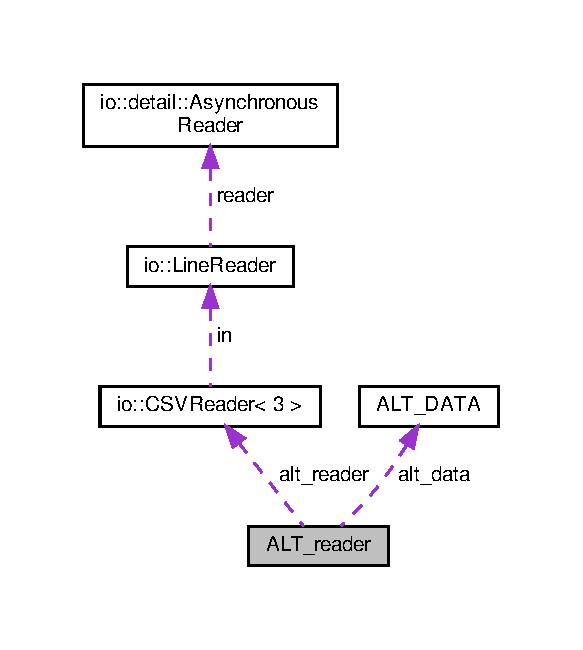
\includegraphics[width=280pt]{classALT__reader__coll__graph}
\end{center}
\end{figure}
\subsection*{Public Member Functions}
\begin{DoxyCompactItemize}
\item 
\mbox{\Hypertarget{classALT__reader_afc32075d3230d4699daa30ffa28fcad3}\label{classALT__reader_afc32075d3230d4699daa30ffa28fcad3}} 
{\bfseries A\+L\+T\+\_\+reader} (std\+::string filename)
\item 
\mbox{\Hypertarget{classALT__reader_a7dfb254b4277f7b559a7a68eef087e58}\label{classALT__reader_a7dfb254b4277f7b559a7a68eef087e58}} 
bool {\bfseries next\+Line} ()
\end{DoxyCompactItemize}
\subsection*{Public Attributes}
\begin{DoxyCompactItemize}
\item 
\mbox{\Hypertarget{classALT__reader_aacaf9a8c099acd10dd53a54ccf564474}\label{classALT__reader_aacaf9a8c099acd10dd53a54ccf564474}} 
\hyperlink{structALT__DATA}{A\+L\+T\+\_\+\+D\+A\+TA} {\bfseries alt\+\_\+data}
\item 
\mbox{\Hypertarget{classALT__reader_a4aac4f3940c04b29d253b10b9e3549e2}\label{classALT__reader_a4aac4f3940c04b29d253b10b9e3549e2}} 
ros\+\_\+float\+::altitude {\bfseries altitude\+Msg}
\item 
\mbox{\Hypertarget{classALT__reader_a9d872dde321d76b2c95a31904b05d2ce}\label{classALT__reader_a9d872dde321d76b2c95a31904b05d2ce}} 
ros\+\_\+float\+::good {\bfseries good\+Msg}
\end{DoxyCompactItemize}
\subsection*{Private Member Functions}
\begin{DoxyCompactItemize}
\item 
\mbox{\Hypertarget{classALT__reader_a99f7700211409858f0989be46f13fb3d}\label{classALT__reader_a99f7700211409858f0989be46f13fb3d}} 
void {\bfseries pack\+\_\+\+Altitude\+\_\+\+Msg} ()
\item 
\mbox{\Hypertarget{classALT__reader_ae28a3371b576983838ea727537967320}\label{classALT__reader_ae28a3371b576983838ea727537967320}} 
void {\bfseries pack\+\_\+\+Good\+\_\+\+Msg} ()
\end{DoxyCompactItemize}
\subsection*{Private Attributes}
\begin{DoxyCompactItemize}
\item 
\mbox{\Hypertarget{classALT__reader_afd2086e0508a80c7c409571b9dbf3449}\label{classALT__reader_afd2086e0508a80c7c409571b9dbf3449}} 
\hyperlink{classio_1_1CSVReader}{io\+::\+C\+S\+V\+Reader}$<$ 3 $>$ {\bfseries alt\+\_\+reader}
\item 
\mbox{\Hypertarget{classALT__reader_a9086f22999868ee6843955edcd23c708}\label{classALT__reader_a9086f22999868ee6843955edcd23c708}} 
unsigned int {\bfseries msg\+Num\+Alt}
\end{DoxyCompactItemize}


The documentation for this class was generated from the following files\+:\begin{DoxyCompactItemize}
\item 
/home/emanuele/catkin\+\_\+ws/src/ros\+\_\+float/include/ros\+\_\+float/alt\+\_\+reader.\+h\item 
/home/emanuele/catkin\+\_\+ws/src/ros\+\_\+float/include/ros\+\_\+float/alt\+\_\+reader.\+cpp\end{DoxyCompactItemize}

\hypertarget{classio_1_1detail_1_1AsynchronousReader}{}\section{io\+:\+:detail\+:\+:Asynchronous\+Reader Class Reference}
\label{classio_1_1detail_1_1AsynchronousReader}\index{io\+::detail\+::\+Asynchronous\+Reader@{io\+::detail\+::\+Asynchronous\+Reader}}
\subsection*{Public Member Functions}
\begin{DoxyCompactItemize}
\item 
\mbox{\Hypertarget{classio_1_1detail_1_1AsynchronousReader_a12ed45f881a671b473d95ded7ad1474c}\label{classio_1_1detail_1_1AsynchronousReader_a12ed45f881a671b473d95ded7ad1474c}} 
void {\bfseries init} (std\+::unique\+\_\+ptr$<$ \hyperlink{classio_1_1ByteSourceBase}{Byte\+Source\+Base} $>$arg\+\_\+byte\+\_\+source)
\item 
\mbox{\Hypertarget{classio_1_1detail_1_1AsynchronousReader_ab6b6f8483008208fc3f529f94c7125e2}\label{classio_1_1detail_1_1AsynchronousReader_ab6b6f8483008208fc3f529f94c7125e2}} 
bool {\bfseries is\+\_\+valid} () const
\item 
\mbox{\Hypertarget{classio_1_1detail_1_1AsynchronousReader_a9818851dbb994042d0d84183220e71c6}\label{classio_1_1detail_1_1AsynchronousReader_a9818851dbb994042d0d84183220e71c6}} 
void {\bfseries start\+\_\+read} (char $\ast$arg\+\_\+buffer, int arg\+\_\+desired\+\_\+byte\+\_\+count)
\item 
\mbox{\Hypertarget{classio_1_1detail_1_1AsynchronousReader_a94520530423e9bfeb04c23ea4e3a8786}\label{classio_1_1detail_1_1AsynchronousReader_a94520530423e9bfeb04c23ea4e3a8786}} 
int {\bfseries finish\+\_\+read} ()
\end{DoxyCompactItemize}
\subsection*{Private Attributes}
\begin{DoxyCompactItemize}
\item 
\mbox{\Hypertarget{classio_1_1detail_1_1AsynchronousReader_a6fd9551f8df07ec6a9ce32f8f33b362d}\label{classio_1_1detail_1_1AsynchronousReader_a6fd9551f8df07ec6a9ce32f8f33b362d}} 
std\+::unique\+\_\+ptr$<$ \hyperlink{classio_1_1ByteSourceBase}{Byte\+Source\+Base} $>$ {\bfseries byte\+\_\+source}
\item 
\mbox{\Hypertarget{classio_1_1detail_1_1AsynchronousReader_a729cf01cc703a42b6010dd5bec4a14f2}\label{classio_1_1detail_1_1AsynchronousReader_a729cf01cc703a42b6010dd5bec4a14f2}} 
std\+::thread {\bfseries worker}
\item 
\mbox{\Hypertarget{classio_1_1detail_1_1AsynchronousReader_a63031e519f616e839031529872bfa164}\label{classio_1_1detail_1_1AsynchronousReader_a63031e519f616e839031529872bfa164}} 
bool {\bfseries termination\+\_\+requested}
\item 
\mbox{\Hypertarget{classio_1_1detail_1_1AsynchronousReader_a6cb2b4a80454dc3b459a378693423a78}\label{classio_1_1detail_1_1AsynchronousReader_a6cb2b4a80454dc3b459a378693423a78}} 
std\+::exception\+\_\+ptr {\bfseries read\+\_\+error}
\item 
\mbox{\Hypertarget{classio_1_1detail_1_1AsynchronousReader_a1b755d751a33453ddaff7974bed29434}\label{classio_1_1detail_1_1AsynchronousReader_a1b755d751a33453ddaff7974bed29434}} 
char $\ast$ {\bfseries buffer}
\item 
\mbox{\Hypertarget{classio_1_1detail_1_1AsynchronousReader_a9bde5d9c5268af659cbb623bea6715fe}\label{classio_1_1detail_1_1AsynchronousReader_a9bde5d9c5268af659cbb623bea6715fe}} 
int {\bfseries desired\+\_\+byte\+\_\+count}
\item 
\mbox{\Hypertarget{classio_1_1detail_1_1AsynchronousReader_ab7aa18093deb7ae67f1c0a699dd4ef93}\label{classio_1_1detail_1_1AsynchronousReader_ab7aa18093deb7ae67f1c0a699dd4ef93}} 
int {\bfseries read\+\_\+byte\+\_\+count}
\item 
\mbox{\Hypertarget{classio_1_1detail_1_1AsynchronousReader_a4fdba0a72e02dd5168b540795acac35e}\label{classio_1_1detail_1_1AsynchronousReader_a4fdba0a72e02dd5168b540795acac35e}} 
std\+::mutex {\bfseries lock}
\item 
\mbox{\Hypertarget{classio_1_1detail_1_1AsynchronousReader_a1ad4bce56a87bb95bae7a21f927c8db0}\label{classio_1_1detail_1_1AsynchronousReader_a1ad4bce56a87bb95bae7a21f927c8db0}} 
std\+::condition\+\_\+variable {\bfseries read\+\_\+finished\+\_\+condition}
\item 
\mbox{\Hypertarget{classio_1_1detail_1_1AsynchronousReader_aaa5c6c774868149377cde2f8857d223d}\label{classio_1_1detail_1_1AsynchronousReader_aaa5c6c774868149377cde2f8857d223d}} 
std\+::condition\+\_\+variable {\bfseries read\+\_\+requested\+\_\+condition}
\end{DoxyCompactItemize}


The documentation for this class was generated from the following file\+:\begin{DoxyCompactItemize}
\item 
/home/emanuele/catkin\+\_\+ws/src/ros\+\_\+float/include/ros\+\_\+float/csv.\+h\end{DoxyCompactItemize}

\hypertarget{structio_1_1error_1_1base}{}\section{io\+:\+:error\+:\+:base Struct Reference}
\label{structio_1_1error_1_1base}\index{io\+::error\+::base@{io\+::error\+::base}}


Inheritance diagram for io\+:\+:error\+:\+:base\+:\nopagebreak
\begin{figure}[H]
\begin{center}
\leavevmode
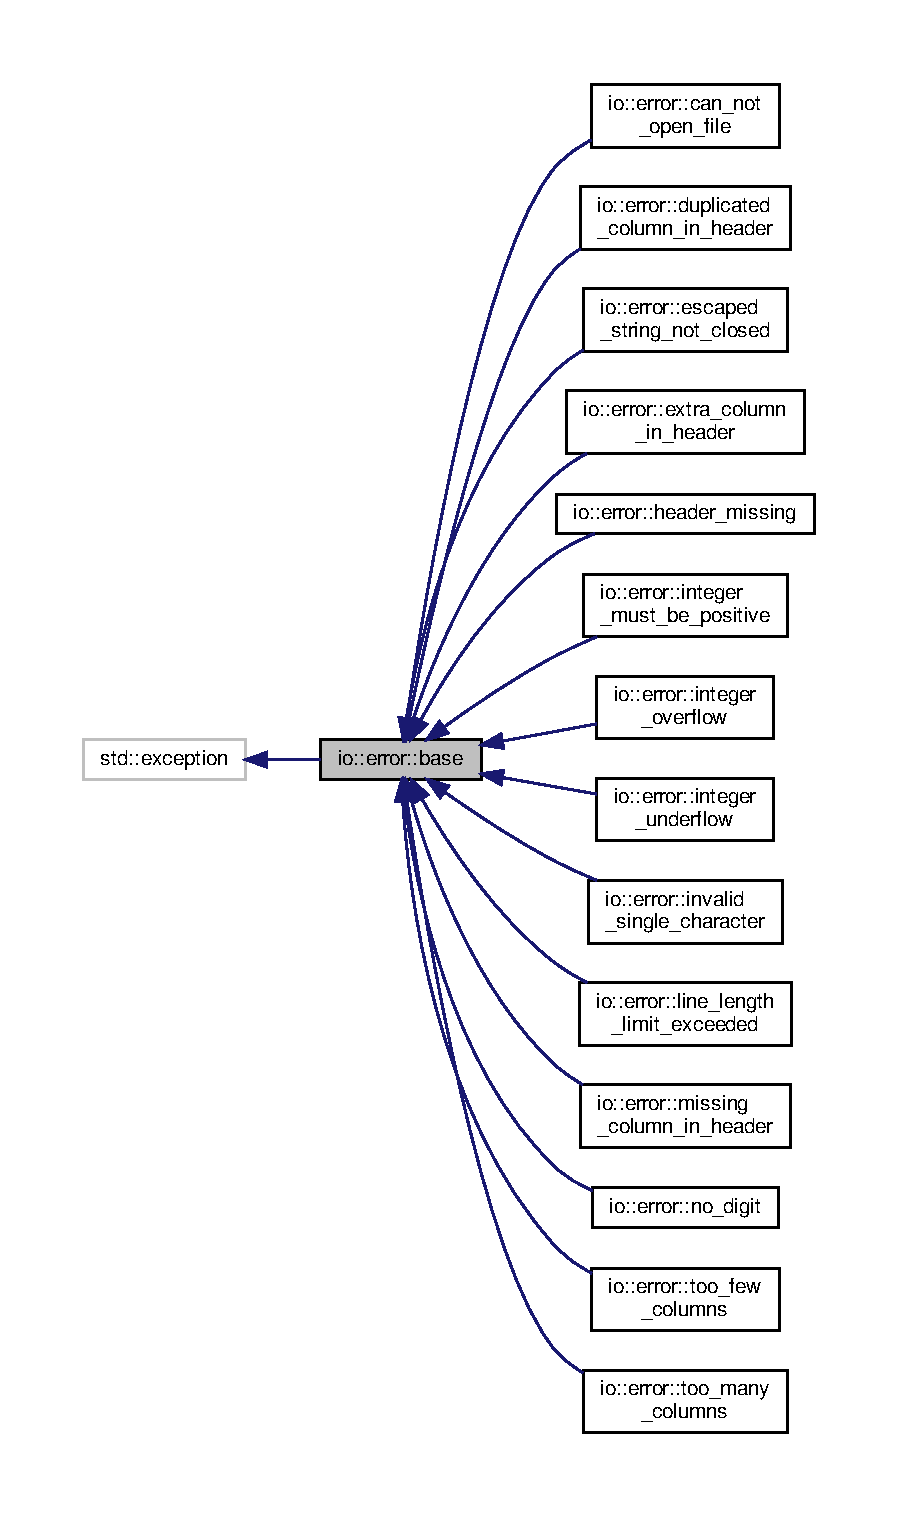
\includegraphics[height=550pt]{structio_1_1error_1_1base__inherit__graph}
\end{center}
\end{figure}


Collaboration diagram for io\+:\+:error\+:\+:base\+:\nopagebreak
\begin{figure}[H]
\begin{center}
\leavevmode
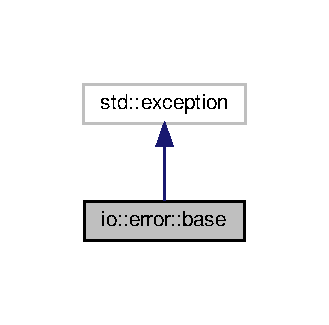
\includegraphics[width=158pt]{structio_1_1error_1_1base__coll__graph}
\end{center}
\end{figure}
\subsection*{Public Member Functions}
\begin{DoxyCompactItemize}
\item 
\mbox{\Hypertarget{structio_1_1error_1_1base_a7d9ff6a31b716a24f056cf8a3e15191d}\label{structio_1_1error_1_1base_a7d9ff6a31b716a24f056cf8a3e15191d}} 
virtual void {\bfseries format\+\_\+error\+\_\+message} () const =0
\item 
\mbox{\Hypertarget{structio_1_1error_1_1base_a35483dfbe91cea45cfa7c5613e83e5ef}\label{structio_1_1error_1_1base_a35483dfbe91cea45cfa7c5613e83e5ef}} 
const char $\ast$ {\bfseries what} () const  throw ()
\end{DoxyCompactItemize}
\subsection*{Public Attributes}
\begin{DoxyCompactItemize}
\item 
\mbox{\Hypertarget{structio_1_1error_1_1base_a3be516c4636b7b61133968cb8081c885}\label{structio_1_1error_1_1base_a3be516c4636b7b61133968cb8081c885}} 
char {\bfseries error\+\_\+message\+\_\+buffer} \mbox{[}512\mbox{]}
\end{DoxyCompactItemize}


The documentation for this struct was generated from the following file\+:\begin{DoxyCompactItemize}
\item 
/home/emanuele/catkin\+\_\+ws/src/ros\+\_\+float/include/ros\+\_\+float/csv.\+h\end{DoxyCompactItemize}

\hypertarget{classio_1_1ByteSourceBase}{}\section{io\+:\+:Byte\+Source\+Base Class Reference}
\label{classio_1_1ByteSourceBase}\index{io\+::\+Byte\+Source\+Base@{io\+::\+Byte\+Source\+Base}}


Inheritance diagram for io\+:\+:Byte\+Source\+Base\+:\nopagebreak
\begin{figure}[H]
\begin{center}
\leavevmode
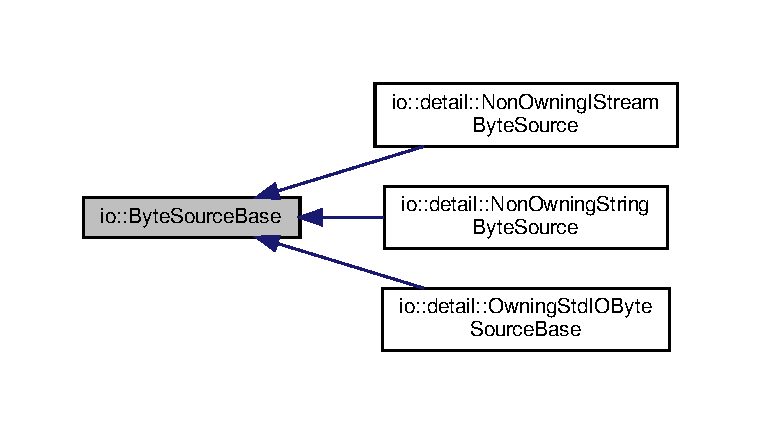
\includegraphics[width=350pt]{classio_1_1ByteSourceBase__inherit__graph}
\end{center}
\end{figure}
\subsection*{Public Member Functions}
\begin{DoxyCompactItemize}
\item 
\mbox{\Hypertarget{classio_1_1ByteSourceBase_a9598bcc869b79e44da07f0e6fa478615}\label{classio_1_1ByteSourceBase_a9598bcc869b79e44da07f0e6fa478615}} 
virtual int {\bfseries read} (char $\ast$buffer, int size)=0
\end{DoxyCompactItemize}


The documentation for this class was generated from the following file\+:\begin{DoxyCompactItemize}
\item 
/home/emanuele/catkin\+\_\+ws/src/ros\+\_\+float/include/ros\+\_\+float/csv.\+h\end{DoxyCompactItemize}

\hypertarget{structio_1_1error_1_1can__not__open__file}{}\section{io\+:\+:error\+:\+:can\+\_\+not\+\_\+open\+\_\+file Struct Reference}
\label{structio_1_1error_1_1can__not__open__file}\index{io\+::error\+::can\+\_\+not\+\_\+open\+\_\+file@{io\+::error\+::can\+\_\+not\+\_\+open\+\_\+file}}


Inheritance diagram for io\+:\+:error\+:\+:can\+\_\+not\+\_\+open\+\_\+file\+:\nopagebreak
\begin{figure}[H]
\begin{center}
\leavevmode
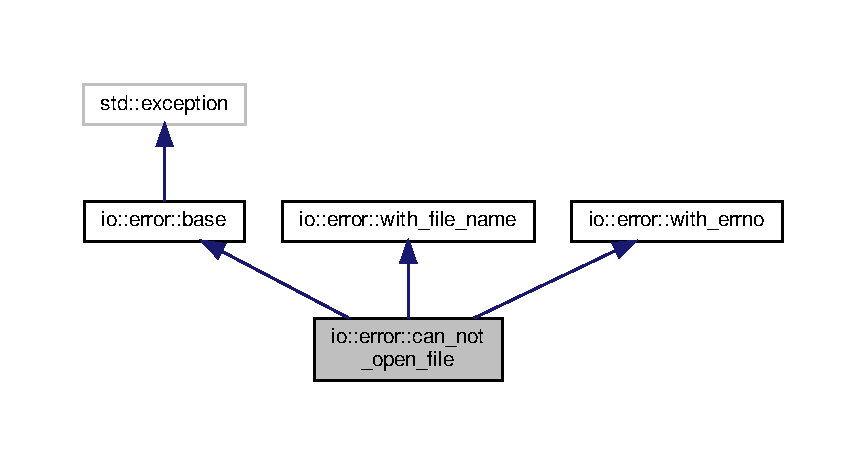
\includegraphics[width=350pt]{structio_1_1error_1_1can__not__open__file__inherit__graph}
\end{center}
\end{figure}


Collaboration diagram for io\+:\+:error\+:\+:can\+\_\+not\+\_\+open\+\_\+file\+:\nopagebreak
\begin{figure}[H]
\begin{center}
\leavevmode
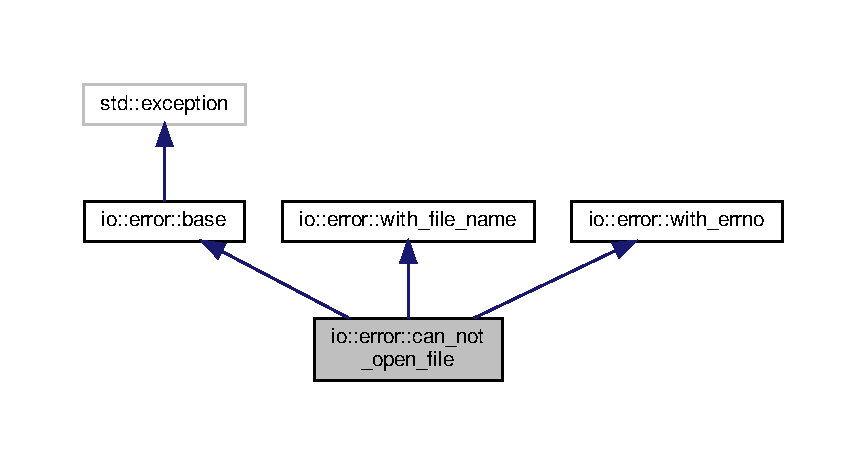
\includegraphics[width=350pt]{structio_1_1error_1_1can__not__open__file__coll__graph}
\end{center}
\end{figure}
\subsection*{Public Member Functions}
\begin{DoxyCompactItemize}
\item 
\mbox{\Hypertarget{structio_1_1error_1_1can__not__open__file_a0249122edaf123e9fa4baabe8128806c}\label{structio_1_1error_1_1can__not__open__file_a0249122edaf123e9fa4baabe8128806c}} 
void {\bfseries format\+\_\+error\+\_\+message} () const
\end{DoxyCompactItemize}
\subsection*{Additional Inherited Members}


The documentation for this struct was generated from the following file\+:\begin{DoxyCompactItemize}
\item 
/home/emanuele/catkin\+\_\+ws/src/ros\+\_\+float/include/ros\+\_\+float/csv.\+h\end{DoxyCompactItemize}

\hypertarget{structCOMMAND__DATA}{}\section{C\+O\+M\+M\+A\+N\+D\+\_\+\+D\+A\+TA Struct Reference}
\label{structCOMMAND__DATA}\index{C\+O\+M\+M\+A\+N\+D\+\_\+\+D\+A\+TA@{C\+O\+M\+M\+A\+N\+D\+\_\+\+D\+A\+TA}}
\subsection*{Public Attributes}
\begin{DoxyCompactItemize}
\item 
\mbox{\Hypertarget{structCOMMAND__DATA_a24645af4764dc230149bb7a05844d640}\label{structCOMMAND__DATA_a24645af4764dc230149bb7a05844d640}} 
unsigned long {\bfseries timestamp}
\item 
\mbox{\Hypertarget{structCOMMAND__DATA_a24e6e2290bcf3727d2e34747a5761252}\label{structCOMMAND__DATA_a24e6e2290bcf3727d2e34747a5761252}} 
int {\bfseries actuator\+\_\+mode}
\item 
\mbox{\Hypertarget{structCOMMAND__DATA_a7bb064d343f24ddec790e4fb0099b299}\label{structCOMMAND__DATA_a7bb064d343f24ddec790e4fb0099b299}} 
int {\bfseries altitude\+\_\+check\+\_\+depth}
\item 
\mbox{\Hypertarget{structCOMMAND__DATA_a5c95967ceccf61847c535d79ceb6e773}\label{structCOMMAND__DATA_a5c95967ceccf61847c535d79ceb6e773}} 
int {\bfseries vel\+\_\+ref}
\item 
\mbox{\Hypertarget{structCOMMAND__DATA_aa5dddce3518074ce18cb7eb1812dc5fc}\label{structCOMMAND__DATA_aa5dddce3518074ce18cb7eb1812dc5fc}} 
int {\bfseries abort}
\item 
\mbox{\Hypertarget{structCOMMAND__DATA_a6f780ee38ec8f930ed096c05111333ee}\label{structCOMMAND__DATA_a6f780ee38ec8f930ed096c05111333ee}} 
int {\bfseries est\+\_\+water\+\_\+depth}
\item 
\mbox{\Hypertarget{structCOMMAND__DATA_a542c4bc095948d8b49308d6d0b6f34be}\label{structCOMMAND__DATA_a542c4bc095948d8b49308d6d0b6f34be}} 
int {\bfseries thrust\+\_\+offset}
\item 
\mbox{\Hypertarget{structCOMMAND__DATA_a6586e78177f3d261d574d4e697a9b6bd}\label{structCOMMAND__DATA_a6586e78177f3d261d574d4e697a9b6bd}} 
double {\bfseries alt\+\_\+ref}
\item 
\mbox{\Hypertarget{structCOMMAND__DATA_a5ead5281cf6875e0a70520da479e71a9}\label{structCOMMAND__DATA_a5ead5281cf6875e0a70520da479e71a9}} 
int {\bfseries ctl\+\_\+active}
\item 
\mbox{\Hypertarget{structCOMMAND__DATA_aa388498d39ba68b844029475340e4e50}\label{structCOMMAND__DATA_aa388498d39ba68b844029475340e4e50}} 
int {\bfseries volume\+\_\+ref}
\item 
\mbox{\Hypertarget{structCOMMAND__DATA_ab390b2dbaa1156a77bf6e3d080af9a35}\label{structCOMMAND__DATA_ab390b2dbaa1156a77bf6e3d080af9a35}} 
int {\bfseries ctl\+\_\+mode\+From\+Command}
\item 
\mbox{\Hypertarget{structCOMMAND__DATA_a9026209f19fb19335030c597bda7ad18}\label{structCOMMAND__DATA_a9026209f19fb19335030c597bda7ad18}} 
int {\bfseries neutral\+\_\+volume}
\item 
\mbox{\Hypertarget{structCOMMAND__DATA_a2609af5c454ba633d2b944ceb129dbe3}\label{structCOMMAND__DATA_a2609af5c454ba633d2b944ceb129dbe3}} 
double {\bfseries thrust\+\_\+ref}
\item 
\mbox{\Hypertarget{structCOMMAND__DATA_aa4a25bc088fa380f1900f6a53e323e85}\label{structCOMMAND__DATA_aa4a25bc088fa380f1900f6a53e323e85}} 
int {\bfseries depth\+\_\+ref}
\item 
\mbox{\Hypertarget{structCOMMAND__DATA_a98b7d0b13fdf01a65ab5e9ddaf8e695e}\label{structCOMMAND__DATA_a98b7d0b13fdf01a65ab5e9ddaf8e695e}} 
int {\bfseries fake\+\_\+altimeter}
\end{DoxyCompactItemize}


The documentation for this struct was generated from the following file\+:\begin{DoxyCompactItemize}
\item 
/home/emanuele/catkin\+\_\+ws/src/ros\+\_\+float/include/ros\+\_\+float/command\+\_\+reader.\+h\end{DoxyCompactItemize}

\hypertarget{classCOMMAND__reader}{}\section{C\+O\+M\+M\+A\+N\+D\+\_\+reader Class Reference}
\label{classCOMMAND__reader}\index{C\+O\+M\+M\+A\+N\+D\+\_\+reader@{C\+O\+M\+M\+A\+N\+D\+\_\+reader}}


Collaboration diagram for C\+O\+M\+M\+A\+N\+D\+\_\+reader\+:\nopagebreak
\begin{figure}[H]
\begin{center}
\leavevmode
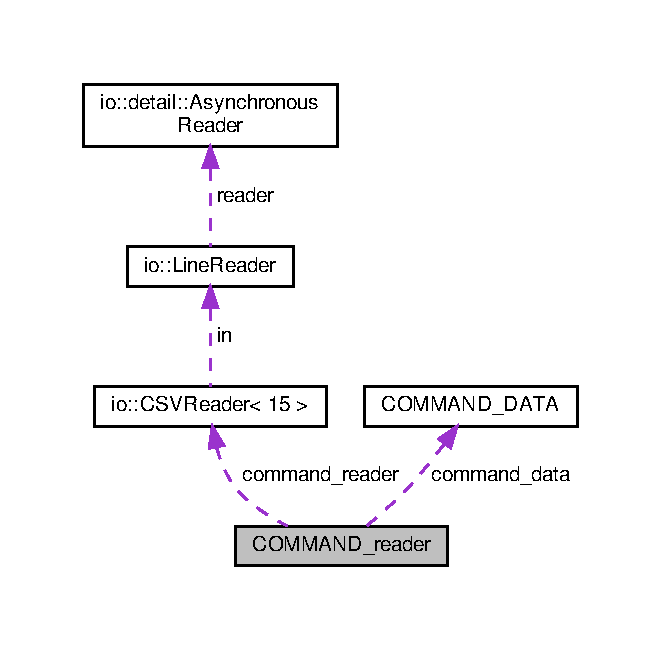
\includegraphics[width=317pt]{classCOMMAND__reader__coll__graph}
\end{center}
\end{figure}
\subsection*{Public Member Functions}
\begin{DoxyCompactItemize}
\item 
\mbox{\Hypertarget{classCOMMAND__reader_ac0f5853e4caf6757c308cbddf0f7af25}\label{classCOMMAND__reader_ac0f5853e4caf6757c308cbddf0f7af25}} 
{\bfseries C\+O\+M\+M\+A\+N\+D\+\_\+reader} (std\+::string filename)
\item 
\mbox{\Hypertarget{classCOMMAND__reader_ad2d61ec5a5af57c09cb3bcefbb3c4629}\label{classCOMMAND__reader_ad2d61ec5a5af57c09cb3bcefbb3c4629}} 
bool {\bfseries next\+Line} ()
\end{DoxyCompactItemize}
\subsection*{Public Attributes}
\begin{DoxyCompactItemize}
\item 
\mbox{\Hypertarget{classCOMMAND__reader_a4c1e6162e78e90e6ba9c6989ac04206a}\label{classCOMMAND__reader_a4c1e6162e78e90e6ba9c6989ac04206a}} 
\hyperlink{structCOMMAND__DATA}{C\+O\+M\+M\+A\+N\+D\+\_\+\+D\+A\+TA} {\bfseries command\+\_\+data}
\item 
\mbox{\Hypertarget{classCOMMAND__reader_a7de64a00033fe9cd465be97ec641079b}\label{classCOMMAND__reader_a7de64a00033fe9cd465be97ec641079b}} 
ros\+\_\+float\+::actuator\+\_\+mode {\bfseries actuator\+Mode\+Msg}
\item 
\mbox{\Hypertarget{classCOMMAND__reader_a9902ff2682bb60a0457973f2592868be}\label{classCOMMAND__reader_a9902ff2682bb60a0457973f2592868be}} 
ros\+\_\+float\+::altitude\+\_\+check\+\_\+depth {\bfseries altitude\+Check\+Depth\+Msg}
\item 
\mbox{\Hypertarget{classCOMMAND__reader_aa40709de3267e5a06a4fa5559d2bf546}\label{classCOMMAND__reader_aa40709de3267e5a06a4fa5559d2bf546}} 
ros\+\_\+float\+::vel\+\_\+ref {\bfseries vel\+Ref\+Msg}
\item 
\mbox{\Hypertarget{classCOMMAND__reader_a47578780050fe7a4ede918a170542dcc}\label{classCOMMAND__reader_a47578780050fe7a4ede918a170542dcc}} 
ros\+\_\+float\+::abort {\bfseries abort\+Msg}
\item 
\mbox{\Hypertarget{classCOMMAND__reader_aa43264cf62d52f91a31e8c65a2e5683d}\label{classCOMMAND__reader_aa43264cf62d52f91a31e8c65a2e5683d}} 
ros\+\_\+float\+::est\+\_\+water\+\_\+depth {\bfseries est\+Water\+Depth\+Msg}
\item 
\mbox{\Hypertarget{classCOMMAND__reader_ade5f822b879e5a91b0eda62430d6487b}\label{classCOMMAND__reader_ade5f822b879e5a91b0eda62430d6487b}} 
ros\+\_\+float\+::thrust\+\_\+offset {\bfseries thrust\+Offset\+Msg}
\item 
\mbox{\Hypertarget{classCOMMAND__reader_a3c89048dd55e02eddaf70ece3f4b3fb0}\label{classCOMMAND__reader_a3c89048dd55e02eddaf70ece3f4b3fb0}} 
ros\+\_\+float\+::alt\+\_\+ref {\bfseries alt\+Ref\+Msg}
\item 
\mbox{\Hypertarget{classCOMMAND__reader_a0cab908689f73d0f9b90b0bcb6f55dbf}\label{classCOMMAND__reader_a0cab908689f73d0f9b90b0bcb6f55dbf}} 
ros\+\_\+float\+::ctl\+\_\+active {\bfseries ctl\+Active\+Msg}
\item 
\mbox{\Hypertarget{classCOMMAND__reader_a4ad0a6dbed5b7fd071379771e6a6f4e7}\label{classCOMMAND__reader_a4ad0a6dbed5b7fd071379771e6a6f4e7}} 
ros\+\_\+float\+::volume\+\_\+ref {\bfseries volume\+Ref\+Msg}
\item 
\mbox{\Hypertarget{classCOMMAND__reader_a5b834059eb8fed6193ee571154ac56ac}\label{classCOMMAND__reader_a5b834059eb8fed6193ee571154ac56ac}} 
ros\+\_\+float\+::ctl\+\_\+mode\+From\+Command {\bfseries ctl\+Mode\+From\+Command\+Msg}
\item 
\mbox{\Hypertarget{classCOMMAND__reader_a52bdc3a18b6e68ab269fad89714633a0}\label{classCOMMAND__reader_a52bdc3a18b6e68ab269fad89714633a0}} 
ros\+\_\+float\+::neutral\+\_\+volume {\bfseries neutral\+Volume\+Msg}
\item 
\mbox{\Hypertarget{classCOMMAND__reader_a53197806107330f5ed1debdb238c4e07}\label{classCOMMAND__reader_a53197806107330f5ed1debdb238c4e07}} 
ros\+\_\+float\+::thrust\+\_\+ref {\bfseries thrust\+Ref\+Msg}
\item 
\mbox{\Hypertarget{classCOMMAND__reader_a1eec4eec1f2d57c803bc97ae12b47f7f}\label{classCOMMAND__reader_a1eec4eec1f2d57c803bc97ae12b47f7f}} 
ros\+\_\+float\+::depth\+\_\+ref {\bfseries depth\+Ref\+Msg}
\item 
\mbox{\Hypertarget{classCOMMAND__reader_a86d2dab939525bfda3357bd75455e551}\label{classCOMMAND__reader_a86d2dab939525bfda3357bd75455e551}} 
ros\+\_\+float\+::fake\+\_\+altimeter {\bfseries fake\+Altimeter\+Msg}
\end{DoxyCompactItemize}
\subsection*{Private Member Functions}
\begin{DoxyCompactItemize}
\item 
\mbox{\Hypertarget{classCOMMAND__reader_ae13f00952dbe6811048be090ceb9879a}\label{classCOMMAND__reader_ae13f00952dbe6811048be090ceb9879a}} 
void {\bfseries pack\+\_\+\+Actuator\+\_\+\+Mode\+\_\+\+Msg} ()
\item 
\mbox{\Hypertarget{classCOMMAND__reader_a685d1fba02464e8a08761f9c0da5f08e}\label{classCOMMAND__reader_a685d1fba02464e8a08761f9c0da5f08e}} 
void {\bfseries pack\+\_\+\+Altitude\+\_\+\+Check\+\_\+\+Depth\+\_\+\+Msg} ()
\item 
\mbox{\Hypertarget{classCOMMAND__reader_aecefb5b993d43831d1f50b33690f539e}\label{classCOMMAND__reader_aecefb5b993d43831d1f50b33690f539e}} 
void {\bfseries pack\+\_\+\+Vel\+\_\+\+Ref\+\_\+\+Msg} ()
\item 
\mbox{\Hypertarget{classCOMMAND__reader_a41f260c4b779dda290f862ad2efa993d}\label{classCOMMAND__reader_a41f260c4b779dda290f862ad2efa993d}} 
void {\bfseries pack\+\_\+\+Abort\+\_\+\+Msg} ()
\item 
\mbox{\Hypertarget{classCOMMAND__reader_ada5b52a230145bdd2d3ee9e9ed9570d6}\label{classCOMMAND__reader_ada5b52a230145bdd2d3ee9e9ed9570d6}} 
void {\bfseries pack\+\_\+\+Est\+\_\+\+Water\+\_\+\+Depth\+\_\+\+Msg} ()
\item 
\mbox{\Hypertarget{classCOMMAND__reader_a6479d37c36364b77c5d6adf2a5edcde0}\label{classCOMMAND__reader_a6479d37c36364b77c5d6adf2a5edcde0}} 
void {\bfseries pack\+\_\+\+Thrust\+\_\+\+Offset\+\_\+\+Msg} ()
\item 
\mbox{\Hypertarget{classCOMMAND__reader_a87f2f4216c7e28ff35e607f68988edd6}\label{classCOMMAND__reader_a87f2f4216c7e28ff35e607f68988edd6}} 
void {\bfseries pack\+\_\+\+Alt\+\_\+\+Ref\+\_\+\+Msg} ()
\item 
\mbox{\Hypertarget{classCOMMAND__reader_a75e1b4110fd01aea6da837dba7fbf680}\label{classCOMMAND__reader_a75e1b4110fd01aea6da837dba7fbf680}} 
void {\bfseries pack\+\_\+\+Ctl\+\_\+\+Active\+\_\+\+Msg} ()
\item 
\mbox{\Hypertarget{classCOMMAND__reader_a23b4fb4512cf9a15370e9a019b7b338f}\label{classCOMMAND__reader_a23b4fb4512cf9a15370e9a019b7b338f}} 
void {\bfseries pack\+\_\+\+Volume\+\_\+\+Ref\+\_\+\+Msg} ()
\item 
\mbox{\Hypertarget{classCOMMAND__reader_af2c35117092d32e5a6404ebe45559178}\label{classCOMMAND__reader_af2c35117092d32e5a6404ebe45559178}} 
void {\bfseries pack\+\_\+\+Ctl\+\_\+\+Mode\+From\+Command\+\_\+\+Msg} ()
\item 
\mbox{\Hypertarget{classCOMMAND__reader_a537401ac7bacba551e48dd03c24657cf}\label{classCOMMAND__reader_a537401ac7bacba551e48dd03c24657cf}} 
void {\bfseries pack\+\_\+\+Neutral\+\_\+\+Volume\+\_\+\+Msg} ()
\item 
\mbox{\Hypertarget{classCOMMAND__reader_a0b3e5e476b7513308c8439d1fb5ea25c}\label{classCOMMAND__reader_a0b3e5e476b7513308c8439d1fb5ea25c}} 
void {\bfseries pack\+\_\+\+Thrust\+\_\+\+Ref\+\_\+\+Msg} ()
\item 
\mbox{\Hypertarget{classCOMMAND__reader_a52e419a1b839ceebc8d10af80b6c4988}\label{classCOMMAND__reader_a52e419a1b839ceebc8d10af80b6c4988}} 
void {\bfseries pack\+\_\+\+Depth\+\_\+\+Ref\+\_\+\+Msg} ()
\item 
\mbox{\Hypertarget{classCOMMAND__reader_a055fb22da6f6f9a770c2c5ef5e7dbf16}\label{classCOMMAND__reader_a055fb22da6f6f9a770c2c5ef5e7dbf16}} 
void {\bfseries pack\+\_\+\+Fake\+\_\+\+A\+Ltimeter} ()
\end{DoxyCompactItemize}
\subsection*{Private Attributes}
\begin{DoxyCompactItemize}
\item 
\mbox{\Hypertarget{classCOMMAND__reader_a10852e59a551516f12c9fac9f5c62bda}\label{classCOMMAND__reader_a10852e59a551516f12c9fac9f5c62bda}} 
\hyperlink{classio_1_1CSVReader}{io\+::\+C\+S\+V\+Reader}$<$ 15 $>$ {\bfseries command\+\_\+reader}
\item 
\mbox{\Hypertarget{classCOMMAND__reader_a80ebeaad902f4058510524210652478f}\label{classCOMMAND__reader_a80ebeaad902f4058510524210652478f}} 
unsigned int {\bfseries msg\+Num\+Command}
\end{DoxyCompactItemize}


The documentation for this class was generated from the following files\+:\begin{DoxyCompactItemize}
\item 
/home/emanuele/catkin\+\_\+ws/src/ros\+\_\+float/include/ros\+\_\+float/command\+\_\+reader.\+h\item 
/home/emanuele/catkin\+\_\+ws/src/ros\+\_\+float/include/ros\+\_\+float/command\+\_\+reader.\+cpp\end{DoxyCompactItemize}

\hypertarget{classio_1_1CSVReader}{}\section{io\+:\+:C\+S\+V\+Reader$<$ column\+\_\+count, trim\+\_\+policy, quote\+\_\+policy, overflow\+\_\+policy, comment\+\_\+policy $>$ Class Template Reference}
\label{classio_1_1CSVReader}\index{io\+::\+C\+S\+V\+Reader$<$ column\+\_\+count, trim\+\_\+policy, quote\+\_\+policy, overflow\+\_\+policy, comment\+\_\+policy $>$@{io\+::\+C\+S\+V\+Reader$<$ column\+\_\+count, trim\+\_\+policy, quote\+\_\+policy, overflow\+\_\+policy, comment\+\_\+policy $>$}}


Collaboration diagram for io\+:\+:C\+S\+V\+Reader$<$ column\+\_\+count, trim\+\_\+policy, quote\+\_\+policy, overflow\+\_\+policy, comment\+\_\+policy $>$\+:\nopagebreak
\begin{figure}[H]
\begin{center}
\leavevmode
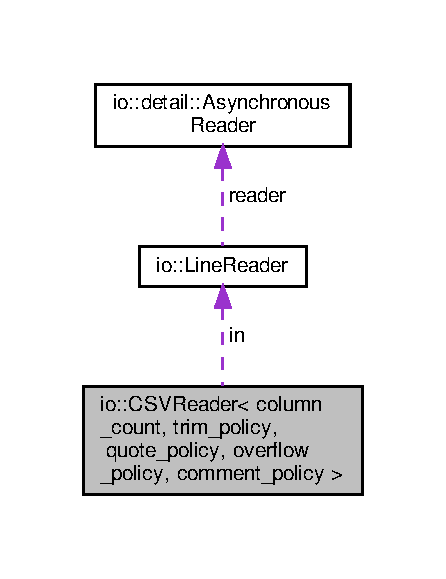
\includegraphics[width=214pt]{classio_1_1CSVReader__coll__graph}
\end{center}
\end{figure}
\subsection*{Public Member Functions}
\begin{DoxyCompactItemize}
\item 
\mbox{\Hypertarget{classio_1_1CSVReader_a0507ac5abe201969a15df76795e13c28}\label{classio_1_1CSVReader_a0507ac5abe201969a15df76795e13c28}} 
{\bfseries C\+S\+V\+Reader} (const \hyperlink{classio_1_1CSVReader}{C\+S\+V\+Reader} \&)=delete
\item 
\mbox{\Hypertarget{classio_1_1CSVReader_a37046e6629cf4254037c14440f14141d}\label{classio_1_1CSVReader_a37046e6629cf4254037c14440f14141d}} 
\hyperlink{classio_1_1CSVReader}{C\+S\+V\+Reader} \& {\bfseries operator=} (const \hyperlink{classio_1_1CSVReader}{C\+S\+V\+Reader} \&)
\item 
\mbox{\Hypertarget{classio_1_1CSVReader_a189debf95672e7cd7582e9f73d7203e5}\label{classio_1_1CSVReader_a189debf95672e7cd7582e9f73d7203e5}} 
{\footnotesize template$<$class ... Args$>$ }\\{\bfseries C\+S\+V\+Reader} (Args \&\&...args)
\item 
\mbox{\Hypertarget{classio_1_1CSVReader_a9fec7797cb27f64360cc48adc5f32c72}\label{classio_1_1CSVReader_a9fec7797cb27f64360cc48adc5f32c72}} 
char $\ast$ {\bfseries next\+\_\+line} ()
\item 
\mbox{\Hypertarget{classio_1_1CSVReader_a9fad9ae02aa243dba6bc78156c5ce7e5}\label{classio_1_1CSVReader_a9fad9ae02aa243dba6bc78156c5ce7e5}} 
{\footnotesize template$<$class ... Col\+Names$>$ }\\void {\bfseries read\+\_\+header} (ignore\+\_\+column ignore\+\_\+policy, Col\+Names...\+cols)
\item 
\mbox{\Hypertarget{classio_1_1CSVReader_ab68eedff1bd59a49fa4ddb160dff94e0}\label{classio_1_1CSVReader_ab68eedff1bd59a49fa4ddb160dff94e0}} 
{\footnotesize template$<$class ... Col\+Names$>$ }\\void {\bfseries set\+\_\+header} (Col\+Names...\+cols)
\item 
\mbox{\Hypertarget{classio_1_1CSVReader_aaba91fff6faea12e451943e8d32a5a17}\label{classio_1_1CSVReader_aaba91fff6faea12e451943e8d32a5a17}} 
bool {\bfseries has\+\_\+column} (const std\+::string \&name) const
\item 
\mbox{\Hypertarget{classio_1_1CSVReader_a4096c1e43a4fba2b4f5ae21d047b5fbc}\label{classio_1_1CSVReader_a4096c1e43a4fba2b4f5ae21d047b5fbc}} 
void {\bfseries set\+\_\+file\+\_\+name} (const std\+::string \&file\+\_\+name)
\item 
\mbox{\Hypertarget{classio_1_1CSVReader_a5f1dc083a8fa8661f5ecdcf6aebc7b24}\label{classio_1_1CSVReader_a5f1dc083a8fa8661f5ecdcf6aebc7b24}} 
void {\bfseries set\+\_\+file\+\_\+name} (const char $\ast$file\+\_\+name)
\item 
\mbox{\Hypertarget{classio_1_1CSVReader_abc6321895152f5a34959b499da6512ee}\label{classio_1_1CSVReader_abc6321895152f5a34959b499da6512ee}} 
const char $\ast$ {\bfseries get\+\_\+truncated\+\_\+file\+\_\+name} () const
\item 
\mbox{\Hypertarget{classio_1_1CSVReader_a1303bd6a2eb0d3d7c743212e52839ac4}\label{classio_1_1CSVReader_a1303bd6a2eb0d3d7c743212e52839ac4}} 
void {\bfseries set\+\_\+file\+\_\+line} (unsigned file\+\_\+line)
\item 
\mbox{\Hypertarget{classio_1_1CSVReader_a065f805596018d1568b81152e6a22e0c}\label{classio_1_1CSVReader_a065f805596018d1568b81152e6a22e0c}} 
unsigned {\bfseries get\+\_\+file\+\_\+line} () const
\item 
\mbox{\Hypertarget{classio_1_1CSVReader_a61ecdcaa62c024bf97c4e5d133478d7e}\label{classio_1_1CSVReader_a61ecdcaa62c024bf97c4e5d133478d7e}} 
{\footnotesize template$<$class ... Col\+Type$>$ }\\bool {\bfseries read\+\_\+row} (Col\+Type \&...cols)
\end{DoxyCompactItemize}
\subsection*{Private Member Functions}
\begin{DoxyCompactItemize}
\item 
\mbox{\Hypertarget{classio_1_1CSVReader_af0f3df423977925fd22acadbdbc4cdcd}\label{classio_1_1CSVReader_af0f3df423977925fd22acadbdbc4cdcd}} 
{\footnotesize template$<$class ... Col\+Names$>$ }\\void {\bfseries set\+\_\+column\+\_\+names} (std\+::string s, Col\+Names...\+cols)
\item 
\mbox{\Hypertarget{classio_1_1CSVReader_a48a56e02ae597ae3506e1b24dc0718ef}\label{classio_1_1CSVReader_a48a56e02ae597ae3506e1b24dc0718ef}} 
void {\bfseries set\+\_\+column\+\_\+names} ()
\item 
\mbox{\Hypertarget{classio_1_1CSVReader_ada16395fbaedad5fcda248b50cd12da0}\label{classio_1_1CSVReader_ada16395fbaedad5fcda248b50cd12da0}} 
void {\bfseries parse\+\_\+helper} (std\+::size\+\_\+t)
\item 
\mbox{\Hypertarget{classio_1_1CSVReader_a6e2cb67ff14a62cee48fb9042c1bfff9}\label{classio_1_1CSVReader_a6e2cb67ff14a62cee48fb9042c1bfff9}} 
{\footnotesize template$<$class T , class ... Col\+Type$>$ }\\void {\bfseries parse\+\_\+helper} (std\+::size\+\_\+t r, T \&t, Col\+Type \&...cols)
\end{DoxyCompactItemize}
\subsection*{Private Attributes}
\begin{DoxyCompactItemize}
\item 
\mbox{\Hypertarget{classio_1_1CSVReader_a26da3892b5c4606617d9daadc0886501}\label{classio_1_1CSVReader_a26da3892b5c4606617d9daadc0886501}} 
\hyperlink{classio_1_1LineReader}{Line\+Reader} {\bfseries in}
\item 
\mbox{\Hypertarget{classio_1_1CSVReader_a48ab5773a4295f7969453838b4115e42}\label{classio_1_1CSVReader_a48ab5773a4295f7969453838b4115e42}} 
char $\ast$ {\bfseries row} \mbox{[}column\+\_\+count\mbox{]}
\item 
\mbox{\Hypertarget{classio_1_1CSVReader_a7b97f929cea543f83e61173ea435fdde}\label{classio_1_1CSVReader_a7b97f929cea543f83e61173ea435fdde}} 
std\+::string {\bfseries column\+\_\+names} \mbox{[}column\+\_\+count\mbox{]}
\item 
\mbox{\Hypertarget{classio_1_1CSVReader_a1a59e51b74c2d6056821a5e499379884}\label{classio_1_1CSVReader_a1a59e51b74c2d6056821a5e499379884}} 
std\+::vector$<$ int $>$ {\bfseries col\+\_\+order}
\end{DoxyCompactItemize}


The documentation for this class was generated from the following file\+:\begin{DoxyCompactItemize}
\item 
/home/emanuele/catkin\+\_\+ws/src/ros\+\_\+float/include/ros\+\_\+float/csv.\+h\end{DoxyCompactItemize}

\hypertarget{structio_1_1double__quote__escape}{}\section{io\+:\+:double\+\_\+quote\+\_\+escape$<$ sep, quote $>$ Struct Template Reference}
\label{structio_1_1double__quote__escape}\index{io\+::double\+\_\+quote\+\_\+escape$<$ sep, quote $>$@{io\+::double\+\_\+quote\+\_\+escape$<$ sep, quote $>$}}
\subsection*{Static Public Member Functions}
\begin{DoxyCompactItemize}
\item 
\mbox{\Hypertarget{structio_1_1double__quote__escape_a30070914039ca8a20f716fbf53d68c41}\label{structio_1_1double__quote__escape_a30070914039ca8a20f716fbf53d68c41}} 
static const char $\ast$ {\bfseries find\+\_\+next\+\_\+column\+\_\+end} (const char $\ast$col\+\_\+begin)
\item 
\mbox{\Hypertarget{structio_1_1double__quote__escape_a02e332751916fbdb7b35c238d690e580}\label{structio_1_1double__quote__escape_a02e332751916fbdb7b35c238d690e580}} 
static void {\bfseries unescape} (char $\ast$\&col\+\_\+begin, char $\ast$\&col\+\_\+end)
\end{DoxyCompactItemize}


The documentation for this struct was generated from the following file\+:\begin{DoxyCompactItemize}
\item 
/home/emanuele/catkin\+\_\+ws/src/ros\+\_\+float/include/ros\+\_\+float/csv.\+h\end{DoxyCompactItemize}

\hypertarget{structio_1_1error_1_1duplicated__column__in__header}{}\section{io\+:\+:error\+:\+:duplicated\+\_\+column\+\_\+in\+\_\+header Struct Reference}
\label{structio_1_1error_1_1duplicated__column__in__header}\index{io\+::error\+::duplicated\+\_\+column\+\_\+in\+\_\+header@{io\+::error\+::duplicated\+\_\+column\+\_\+in\+\_\+header}}


Inheritance diagram for io\+:\+:error\+:\+:duplicated\+\_\+column\+\_\+in\+\_\+header\+:\nopagebreak
\begin{figure}[H]
\begin{center}
\leavevmode
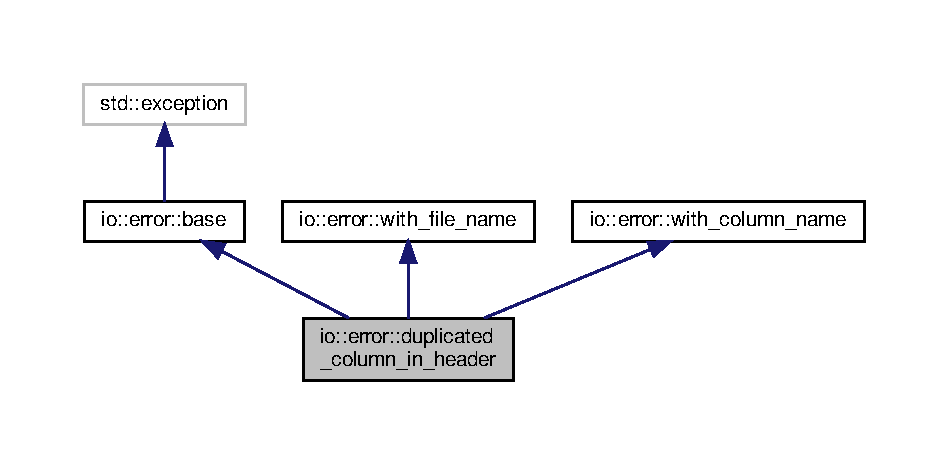
\includegraphics[width=350pt]{structio_1_1error_1_1duplicated__column__in__header__inherit__graph}
\end{center}
\end{figure}


Collaboration diagram for io\+:\+:error\+:\+:duplicated\+\_\+column\+\_\+in\+\_\+header\+:\nopagebreak
\begin{figure}[H]
\begin{center}
\leavevmode
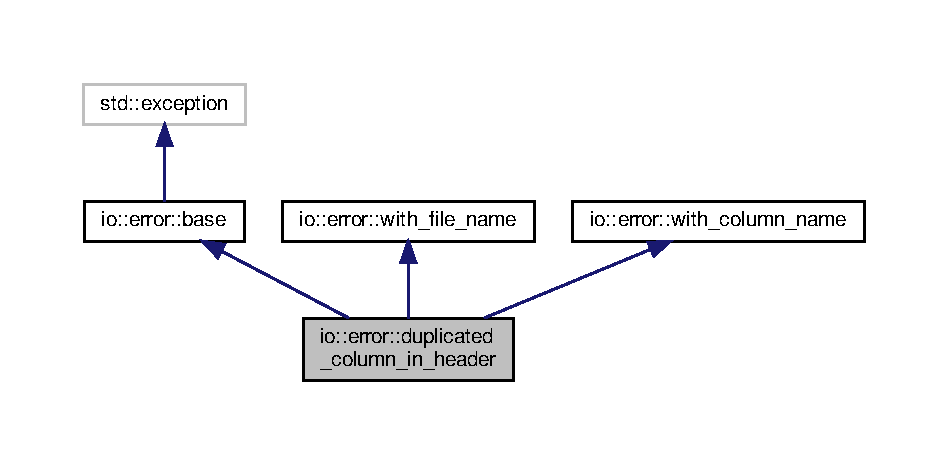
\includegraphics[width=350pt]{structio_1_1error_1_1duplicated__column__in__header__coll__graph}
\end{center}
\end{figure}
\subsection*{Public Member Functions}
\begin{DoxyCompactItemize}
\item 
\mbox{\Hypertarget{structio_1_1error_1_1duplicated__column__in__header_a213825695d770d3ee2ee7bb9a2bfa818}\label{structio_1_1error_1_1duplicated__column__in__header_a213825695d770d3ee2ee7bb9a2bfa818}} 
void {\bfseries format\+\_\+error\+\_\+message} () const
\end{DoxyCompactItemize}
\subsection*{Additional Inherited Members}


The documentation for this struct was generated from the following file\+:\begin{DoxyCompactItemize}
\item 
/home/emanuele/catkin\+\_\+ws/src/ros\+\_\+float/include/ros\+\_\+float/csv.\+h\end{DoxyCompactItemize}

\hypertarget{structio_1_1empty__line__comment}{}\section{io\+:\+:empty\+\_\+line\+\_\+comment Struct Reference}
\label{structio_1_1empty__line__comment}\index{io\+::empty\+\_\+line\+\_\+comment@{io\+::empty\+\_\+line\+\_\+comment}}
\subsection*{Static Public Member Functions}
\begin{DoxyCompactItemize}
\item 
\mbox{\Hypertarget{structio_1_1empty__line__comment_a88e2cee044a9aafabf3e2a0e64fa5289}\label{structio_1_1empty__line__comment_a88e2cee044a9aafabf3e2a0e64fa5289}} 
static bool {\bfseries is\+\_\+comment} (const char $\ast$line)
\end{DoxyCompactItemize}


The documentation for this struct was generated from the following file\+:\begin{DoxyCompactItemize}
\item 
/home/emanuele/catkin\+\_\+ws/src/ros\+\_\+float/include/ros\+\_\+float/csv.\+h\end{DoxyCompactItemize}

\hypertarget{structio_1_1error_1_1escaped__string__not__closed}{}\section{io\+:\+:error\+:\+:escaped\+\_\+string\+\_\+not\+\_\+closed Struct Reference}
\label{structio_1_1error_1_1escaped__string__not__closed}\index{io\+::error\+::escaped\+\_\+string\+\_\+not\+\_\+closed@{io\+::error\+::escaped\+\_\+string\+\_\+not\+\_\+closed}}


Inheritance diagram for io\+:\+:error\+:\+:escaped\+\_\+string\+\_\+not\+\_\+closed\+:\nopagebreak
\begin{figure}[H]
\begin{center}
\leavevmode
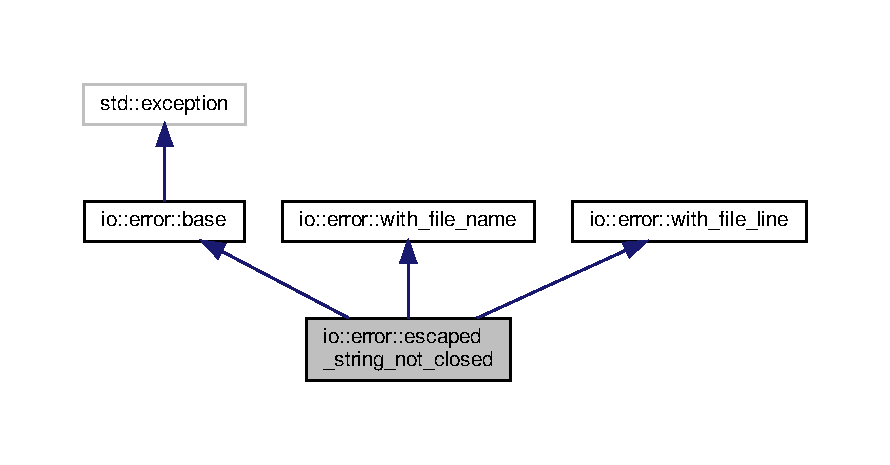
\includegraphics[width=350pt]{structio_1_1error_1_1escaped__string__not__closed__inherit__graph}
\end{center}
\end{figure}


Collaboration diagram for io\+:\+:error\+:\+:escaped\+\_\+string\+\_\+not\+\_\+closed\+:\nopagebreak
\begin{figure}[H]
\begin{center}
\leavevmode
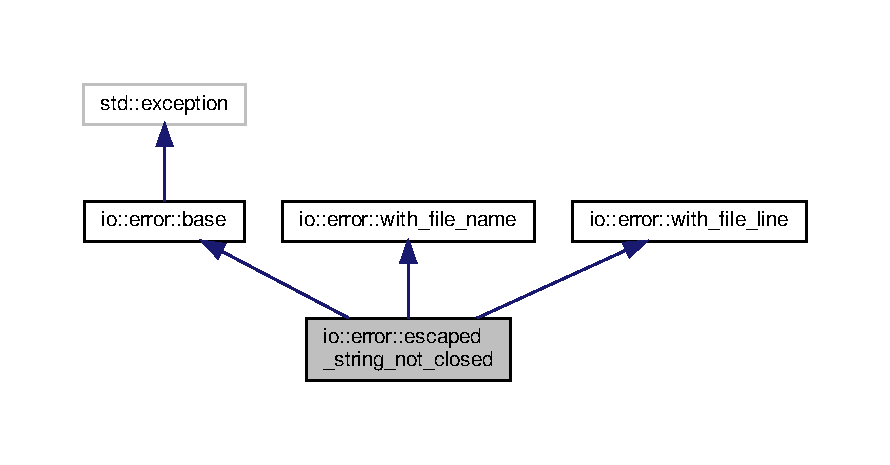
\includegraphics[width=350pt]{structio_1_1error_1_1escaped__string__not__closed__coll__graph}
\end{center}
\end{figure}
\subsection*{Public Member Functions}
\begin{DoxyCompactItemize}
\item 
\mbox{\Hypertarget{structio_1_1error_1_1escaped__string__not__closed_a696911cd3cfaf8a30a728101b076028d}\label{structio_1_1error_1_1escaped__string__not__closed_a696911cd3cfaf8a30a728101b076028d}} 
void {\bfseries format\+\_\+error\+\_\+message} () const
\end{DoxyCompactItemize}
\subsection*{Additional Inherited Members}


The documentation for this struct was generated from the following file\+:\begin{DoxyCompactItemize}
\item 
/home/emanuele/catkin\+\_\+ws/src/ros\+\_\+float/include/ros\+\_\+float/csv.\+h\end{DoxyCompactItemize}

\hypertarget{structio_1_1error_1_1extra__column__in__header}{}\section{io\+:\+:error\+:\+:extra\+\_\+column\+\_\+in\+\_\+header Struct Reference}
\label{structio_1_1error_1_1extra__column__in__header}\index{io\+::error\+::extra\+\_\+column\+\_\+in\+\_\+header@{io\+::error\+::extra\+\_\+column\+\_\+in\+\_\+header}}


Inheritance diagram for io\+:\+:error\+:\+:extra\+\_\+column\+\_\+in\+\_\+header\+:\nopagebreak
\begin{figure}[H]
\begin{center}
\leavevmode
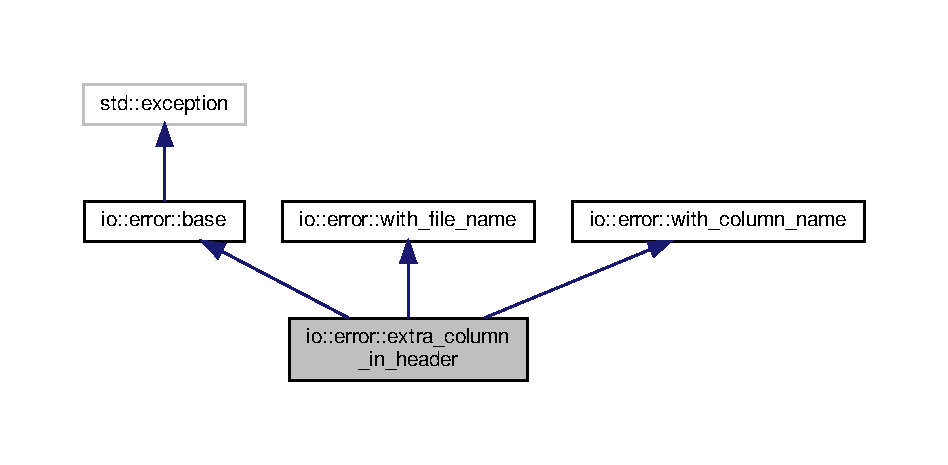
\includegraphics[width=350pt]{structio_1_1error_1_1extra__column__in__header__inherit__graph}
\end{center}
\end{figure}


Collaboration diagram for io\+:\+:error\+:\+:extra\+\_\+column\+\_\+in\+\_\+header\+:\nopagebreak
\begin{figure}[H]
\begin{center}
\leavevmode
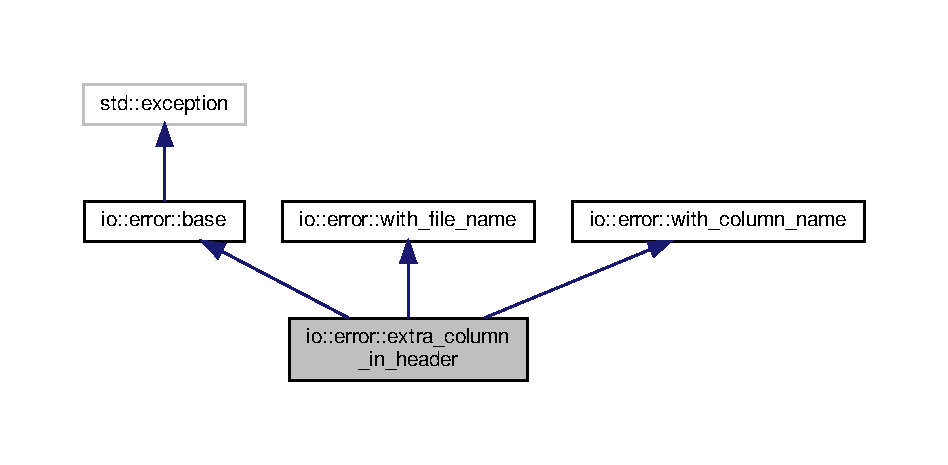
\includegraphics[width=350pt]{structio_1_1error_1_1extra__column__in__header__coll__graph}
\end{center}
\end{figure}
\subsection*{Public Member Functions}
\begin{DoxyCompactItemize}
\item 
\mbox{\Hypertarget{structio_1_1error_1_1extra__column__in__header_ab7bb962a470c429206c51729fbf114dd}\label{structio_1_1error_1_1extra__column__in__header_ab7bb962a470c429206c51729fbf114dd}} 
void {\bfseries format\+\_\+error\+\_\+message} () const
\end{DoxyCompactItemize}
\subsection*{Additional Inherited Members}


The documentation for this struct was generated from the following file\+:\begin{DoxyCompactItemize}
\item 
/home/emanuele/catkin\+\_\+ws/src/ros\+\_\+float/include/ros\+\_\+float/csv.\+h\end{DoxyCompactItemize}

\hypertarget{structGPS__DATA}{}\section{G\+P\+S\+\_\+\+D\+A\+TA Struct Reference}
\label{structGPS__DATA}\index{G\+P\+S\+\_\+\+D\+A\+TA@{G\+P\+S\+\_\+\+D\+A\+TA}}
\subsection*{Public Attributes}
\begin{DoxyCompactItemize}
\item 
\mbox{\Hypertarget{structGPS__DATA_a8b47080424717840dcd1d7735966a35e}\label{structGPS__DATA_a8b47080424717840dcd1d7735966a35e}} 
double {\bfseries latitude}
\item 
\mbox{\Hypertarget{structGPS__DATA_aacdddf8ba4d5421d79f9743802282059}\label{structGPS__DATA_aacdddf8ba4d5421d79f9743802282059}} 
double {\bfseries longitude}
\item 
\mbox{\Hypertarget{structGPS__DATA_a267d72bc5ffa62d95a436a0f3174880b}\label{structGPS__DATA_a267d72bc5ffa62d95a436a0f3174880b}} 
unsigned long {\bfseries timestamp}
\item 
\mbox{\Hypertarget{structGPS__DATA_ae4b07b5117bf09d17562a444e9008b5b}\label{structGPS__DATA_ae4b07b5117bf09d17562a444e9008b5b}} 
int {\bfseries status}
\item 
\mbox{\Hypertarget{structGPS__DATA_a0ae225b2748132bcc53492ae77beed21}\label{structGPS__DATA_a0ae225b2748132bcc53492ae77beed21}} 
double {\bfseries sog}
\item 
\mbox{\Hypertarget{structGPS__DATA_a5d801c847ed250f719ddbc6bef40747a}\label{structGPS__DATA_a5d801c847ed250f719ddbc6bef40747a}} 
double {\bfseries cmg}
\item 
\mbox{\Hypertarget{structGPS__DATA_a78c013260c16e31689f465b13dbd4181}\label{structGPS__DATA_a78c013260c16e31689f465b13dbd4181}} 
int {\bfseries gps\+\_\+timestamp}
\item 
\mbox{\Hypertarget{structGPS__DATA_a23978978be610dac2f247312bb1b32e1}\label{structGPS__DATA_a23978978be610dac2f247312bb1b32e1}} 
int {\bfseries magvar}
\end{DoxyCompactItemize}


The documentation for this struct was generated from the following file\+:\begin{DoxyCompactItemize}
\item 
/home/emanuele/catkin\+\_\+ws/src/ros\+\_\+float/include/ros\+\_\+float/gps\+\_\+reader.\+h\end{DoxyCompactItemize}

\hypertarget{classGPS__reader}{}\section{G\+P\+S\+\_\+reader Class Reference}
\label{classGPS__reader}\index{G\+P\+S\+\_\+reader@{G\+P\+S\+\_\+reader}}


Collaboration diagram for G\+P\+S\+\_\+reader\+:\nopagebreak
\begin{figure}[H]
\begin{center}
\leavevmode
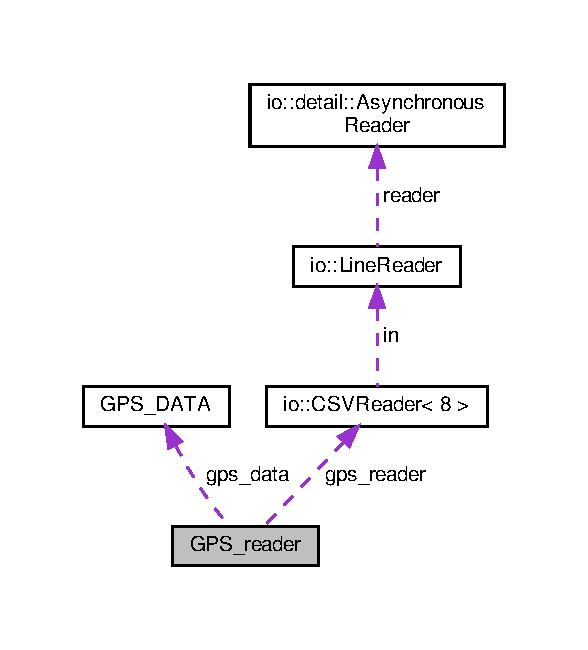
\includegraphics[width=282pt]{classGPS__reader__coll__graph}
\end{center}
\end{figure}
\subsection*{Public Member Functions}
\begin{DoxyCompactItemize}
\item 
\mbox{\Hypertarget{classGPS__reader_aea612c431bf535d34779946b1eaf17f0}\label{classGPS__reader_aea612c431bf535d34779946b1eaf17f0}} 
{\bfseries G\+P\+S\+\_\+reader} (std\+::string filename)
\item 
\mbox{\Hypertarget{classGPS__reader_a3b0ee842ec5fb7d632dbea4e3be04365}\label{classGPS__reader_a3b0ee842ec5fb7d632dbea4e3be04365}} 
bool {\bfseries next\+Line} ()
\end{DoxyCompactItemize}
\subsection*{Public Attributes}
\begin{DoxyCompactItemize}
\item 
\mbox{\Hypertarget{classGPS__reader_a105510384a32f68ba0b2071802a67ef2}\label{classGPS__reader_a105510384a32f68ba0b2071802a67ef2}} 
\hyperlink{structGPS__DATA}{G\+P\+S\+\_\+\+D\+A\+TA} {\bfseries gps\+\_\+data}
\item 
\mbox{\Hypertarget{classGPS__reader_ab08127115b385e07851bb4b6c8492473}\label{classGPS__reader_ab08127115b385e07851bb4b6c8492473}} 
ros\+\_\+float\+::cmg {\bfseries cmg\+Msg}
\item 
\mbox{\Hypertarget{classGPS__reader_a8f04f46e401652161415b0c73c1a5b00}\label{classGPS__reader_a8f04f46e401652161415b0c73c1a5b00}} 
ros\+\_\+float\+::gps\+\_\+timestamp {\bfseries gps\+\_\+time\+Msg}
\item 
\mbox{\Hypertarget{classGPS__reader_ab97b67a2e2646df6956bcc080fe8d687}\label{classGPS__reader_ab97b67a2e2646df6956bcc080fe8d687}} 
ros\+\_\+float\+::mag\+\_\+var {\bfseries magvar\+Msg}
\item 
\mbox{\Hypertarget{classGPS__reader_a4f6b645cee68742e584c36498d4bd683}\label{classGPS__reader_a4f6b645cee68742e584c36498d4bd683}} 
ros\+\_\+float\+::sog {\bfseries sog\+Msg}
\item 
\mbox{\Hypertarget{classGPS__reader_a6c5001bfda4b20c8c627e84240ebf87a}\label{classGPS__reader_a6c5001bfda4b20c8c627e84240ebf87a}} 
sensor\+\_\+msgs\+::\+Nav\+Sat\+Fix {\bfseries fix\+Msg}
\end{DoxyCompactItemize}
\subsection*{Private Member Functions}
\begin{DoxyCompactItemize}
\item 
void \hyperlink{classGPS__reader_a548d1980ea97af075804d34638af3a26}{pack\+Fix\+Msg} ()
\begin{DoxyCompactList}\small\item\em Packs up fix message from input file. \end{DoxyCompactList}\item 
\mbox{\Hypertarget{classGPS__reader_ad88607d8d71d056ade5dc69dc02fced3}\label{classGPS__reader_ad88607d8d71d056ade5dc69dc02fced3}} 
void {\bfseries pack\+Lat\+Msg} ()
\item 
\mbox{\Hypertarget{classGPS__reader_a452eaf0edee31f3feb2b958e9310aff3}\label{classGPS__reader_a452eaf0edee31f3feb2b958e9310aff3}} 
void {\bfseries pack\+Lon\+Msg} ()
\item 
\mbox{\Hypertarget{classGPS__reader_a67385f5ba46b5d866a36d1b0b63d4e23}\label{classGPS__reader_a67385f5ba46b5d866a36d1b0b63d4e23}} 
void {\bfseries pack\+Status} ()
\item 
\mbox{\Hypertarget{classGPS__reader_a057566cd28481e2b265da7c7bc5094f4}\label{classGPS__reader_a057566cd28481e2b265da7c7bc5094f4}} 
void {\bfseries pack\+G\+P\+S\+\_\+\+Timestamp} ()
\item 
\mbox{\Hypertarget{classGPS__reader_a4d3cd1b5b65b45bdc873063903ac5ee6}\label{classGPS__reader_a4d3cd1b5b65b45bdc873063903ac5ee6}} 
void {\bfseries pack\+Sog\+Msg} ()
\item 
\mbox{\Hypertarget{classGPS__reader_ac0aad343dff364ccc5acff3a8f1951d0}\label{classGPS__reader_ac0aad343dff364ccc5acff3a8f1951d0}} 
void {\bfseries pack\+Cmg\+Msg} ()
\item 
\mbox{\Hypertarget{classGPS__reader_ac682fedffe40ef0f86c574e065a81910}\label{classGPS__reader_ac682fedffe40ef0f86c574e065a81910}} 
void {\bfseries pack\+Mag\+Var\+Msg} ()
\end{DoxyCompactItemize}
\subsection*{Private Attributes}
\begin{DoxyCompactItemize}
\item 
\mbox{\Hypertarget{classGPS__reader_a83dc8c11a68339ff3c14ec1f4cc14d50}\label{classGPS__reader_a83dc8c11a68339ff3c14ec1f4cc14d50}} 
\hyperlink{classio_1_1CSVReader}{io\+::\+C\+S\+V\+Reader}$<$ 8 $>$ {\bfseries gps\+\_\+reader}
\item 
\mbox{\Hypertarget{classGPS__reader_a11c923e2668986841cdb75976f8b4c8a}\label{classGPS__reader_a11c923e2668986841cdb75976f8b4c8a}} 
unsigned int {\bfseries msg\+Num\+G\+PS}
\end{DoxyCompactItemize}


\subsection{Member Function Documentation}
\mbox{\Hypertarget{classGPS__reader_a548d1980ea97af075804d34638af3a26}\label{classGPS__reader_a548d1980ea97af075804d34638af3a26}} 
\index{G\+P\+S\+\_\+reader@{G\+P\+S\+\_\+reader}!pack\+Fix\+Msg@{pack\+Fix\+Msg}}
\index{pack\+Fix\+Msg@{pack\+Fix\+Msg}!G\+P\+S\+\_\+reader@{G\+P\+S\+\_\+reader}}
\subsubsection{\texorpdfstring{pack\+Fix\+Msg()}{packFixMsg()}}
{\footnotesize\ttfamily void G\+P\+S\+\_\+reader\+::pack\+Fix\+Msg (\begin{DoxyParamCaption}{ }\end{DoxyParamCaption})\hspace{0.3cm}{\ttfamily [private]}}



Packs up fix message from input file. 

\begin{DoxyRefDesc}{Todo}
\item[\hyperlink{todo__todo000001}{Todo}]ask croman for conformation \end{DoxyRefDesc}


The documentation for this class was generated from the following files\+:\begin{DoxyCompactItemize}
\item 
/home/emanuele/catkin\+\_\+ws/src/ros\+\_\+float/include/ros\+\_\+float/gps\+\_\+reader.\+h\item 
/home/emanuele/catkin\+\_\+ws/src/ros\+\_\+float/include/ros\+\_\+float/gps\+\_\+reader.\+cpp\end{DoxyCompactItemize}

\hypertarget{structio_1_1error_1_1header__missing}{}\section{io\+:\+:error\+:\+:header\+\_\+missing Struct Reference}
\label{structio_1_1error_1_1header__missing}\index{io\+::error\+::header\+\_\+missing@{io\+::error\+::header\+\_\+missing}}


Inheritance diagram for io\+:\+:error\+:\+:header\+\_\+missing\+:\nopagebreak
\begin{figure}[H]
\begin{center}
\leavevmode
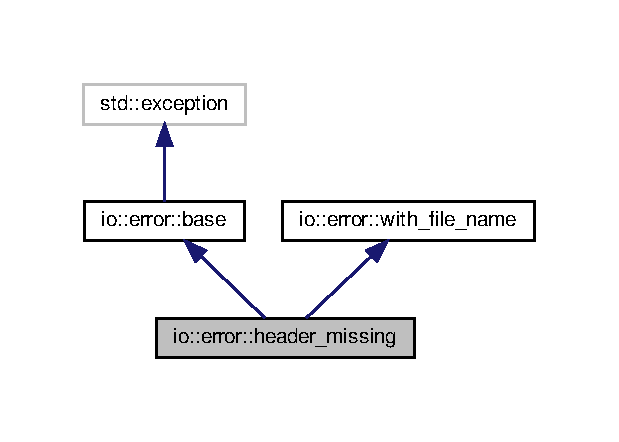
\includegraphics[width=297pt]{structio_1_1error_1_1header__missing__inherit__graph}
\end{center}
\end{figure}


Collaboration diagram for io\+:\+:error\+:\+:header\+\_\+missing\+:\nopagebreak
\begin{figure}[H]
\begin{center}
\leavevmode
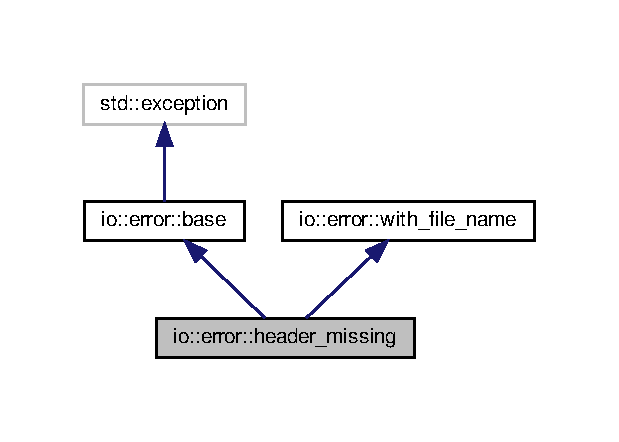
\includegraphics[width=297pt]{structio_1_1error_1_1header__missing__coll__graph}
\end{center}
\end{figure}
\subsection*{Public Member Functions}
\begin{DoxyCompactItemize}
\item 
\mbox{\Hypertarget{structio_1_1error_1_1header__missing_ae130d632556617cf136cc4392b517b30}\label{structio_1_1error_1_1header__missing_ae130d632556617cf136cc4392b517b30}} 
void {\bfseries format\+\_\+error\+\_\+message} () const
\end{DoxyCompactItemize}
\subsection*{Additional Inherited Members}


The documentation for this struct was generated from the following file\+:\begin{DoxyCompactItemize}
\item 
/home/emanuele/catkin\+\_\+ws/src/ros\+\_\+float/include/ros\+\_\+float/csv.\+h\end{DoxyCompactItemize}

\hypertarget{structio_1_1ignore__overflow}{}\section{io\+:\+:ignore\+\_\+overflow Struct Reference}
\label{structio_1_1ignore__overflow}\index{io\+::ignore\+\_\+overflow@{io\+::ignore\+\_\+overflow}}
\subsection*{Static Public Member Functions}
\begin{DoxyCompactItemize}
\item 
\mbox{\Hypertarget{structio_1_1ignore__overflow_aed3e5026cfa7157ea9270ae377d1026b}\label{structio_1_1ignore__overflow_aed3e5026cfa7157ea9270ae377d1026b}} 
{\footnotesize template$<$class T $>$ }\\static void {\bfseries on\+\_\+overflow} (T \&)
\item 
\mbox{\Hypertarget{structio_1_1ignore__overflow_aece692f7a20933149ec99aa1f97458ad}\label{structio_1_1ignore__overflow_aece692f7a20933149ec99aa1f97458ad}} 
{\footnotesize template$<$class T $>$ }\\static void {\bfseries on\+\_\+underflow} (T \&)
\end{DoxyCompactItemize}


The documentation for this struct was generated from the following file\+:\begin{DoxyCompactItemize}
\item 
/home/emanuele/catkin\+\_\+ws/src/ros\+\_\+float/include/ros\+\_\+float/csv.\+h\end{DoxyCompactItemize}

\hypertarget{structio_1_1error_1_1integer__must__be__positive}{}\section{io\+:\+:error\+:\+:integer\+\_\+must\+\_\+be\+\_\+positive Struct Reference}
\label{structio_1_1error_1_1integer__must__be__positive}\index{io\+::error\+::integer\+\_\+must\+\_\+be\+\_\+positive@{io\+::error\+::integer\+\_\+must\+\_\+be\+\_\+positive}}


Inheritance diagram for io\+:\+:error\+:\+:integer\+\_\+must\+\_\+be\+\_\+positive\+:\nopagebreak
\begin{figure}[H]
\begin{center}
\leavevmode
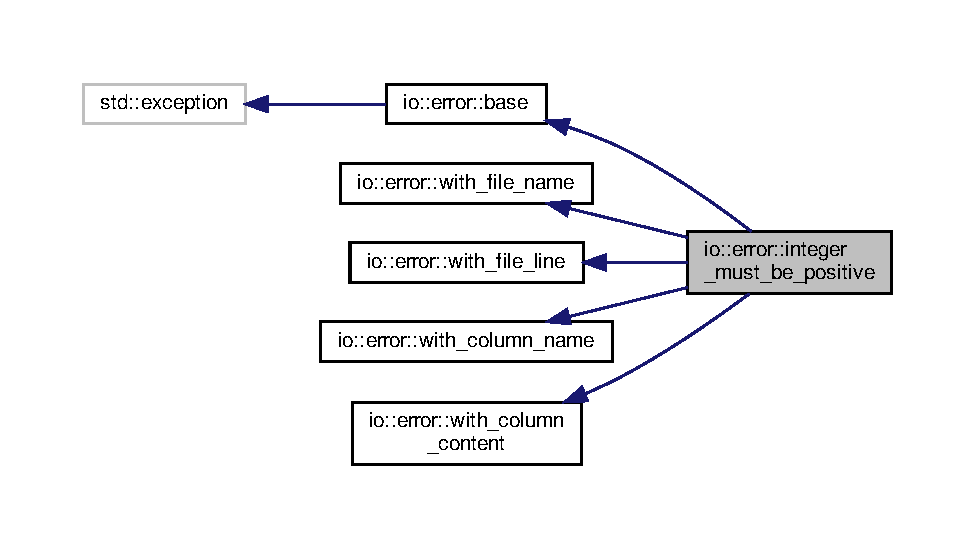
\includegraphics[width=350pt]{structio_1_1error_1_1integer__must__be__positive__inherit__graph}
\end{center}
\end{figure}


Collaboration diagram for io\+:\+:error\+:\+:integer\+\_\+must\+\_\+be\+\_\+positive\+:\nopagebreak
\begin{figure}[H]
\begin{center}
\leavevmode
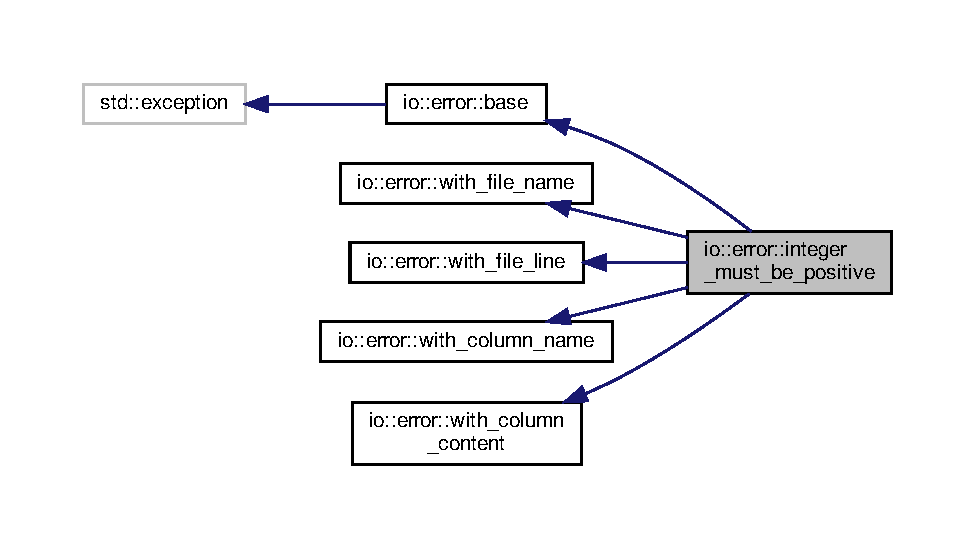
\includegraphics[width=350pt]{structio_1_1error_1_1integer__must__be__positive__coll__graph}
\end{center}
\end{figure}
\subsection*{Public Member Functions}
\begin{DoxyCompactItemize}
\item 
\mbox{\Hypertarget{structio_1_1error_1_1integer__must__be__positive_af6daaa02512141958a3eafd0c07232ef}\label{structio_1_1error_1_1integer__must__be__positive_af6daaa02512141958a3eafd0c07232ef}} 
void {\bfseries format\+\_\+error\+\_\+message} () const
\end{DoxyCompactItemize}
\subsection*{Additional Inherited Members}


The documentation for this struct was generated from the following file\+:\begin{DoxyCompactItemize}
\item 
/home/emanuele/catkin\+\_\+ws/src/ros\+\_\+float/include/ros\+\_\+float/csv.\+h\end{DoxyCompactItemize}

\hypertarget{structio_1_1error_1_1integer__overflow}{}\section{io\+:\+:error\+:\+:integer\+\_\+overflow Struct Reference}
\label{structio_1_1error_1_1integer__overflow}\index{io\+::error\+::integer\+\_\+overflow@{io\+::error\+::integer\+\_\+overflow}}


Inheritance diagram for io\+:\+:error\+:\+:integer\+\_\+overflow\+:\nopagebreak
\begin{figure}[H]
\begin{center}
\leavevmode
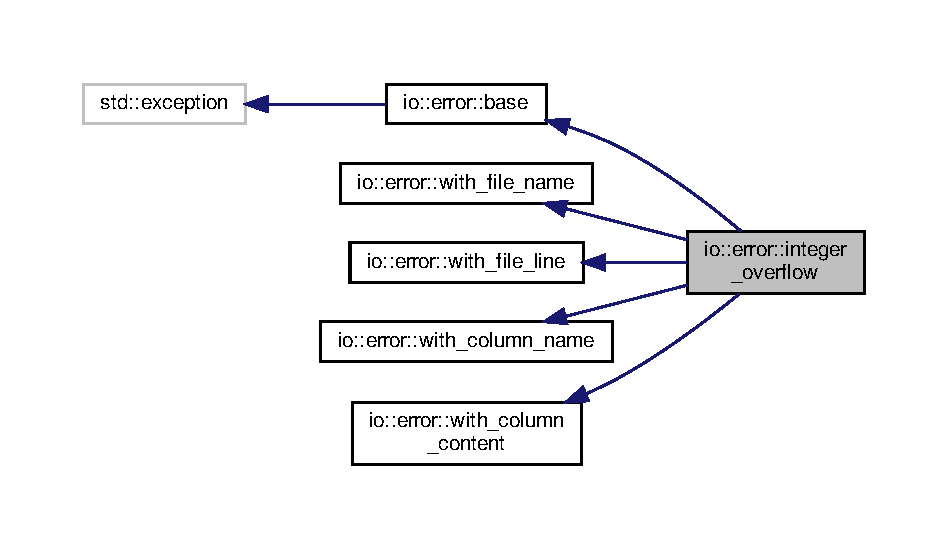
\includegraphics[width=350pt]{structio_1_1error_1_1integer__overflow__inherit__graph}
\end{center}
\end{figure}


Collaboration diagram for io\+:\+:error\+:\+:integer\+\_\+overflow\+:\nopagebreak
\begin{figure}[H]
\begin{center}
\leavevmode
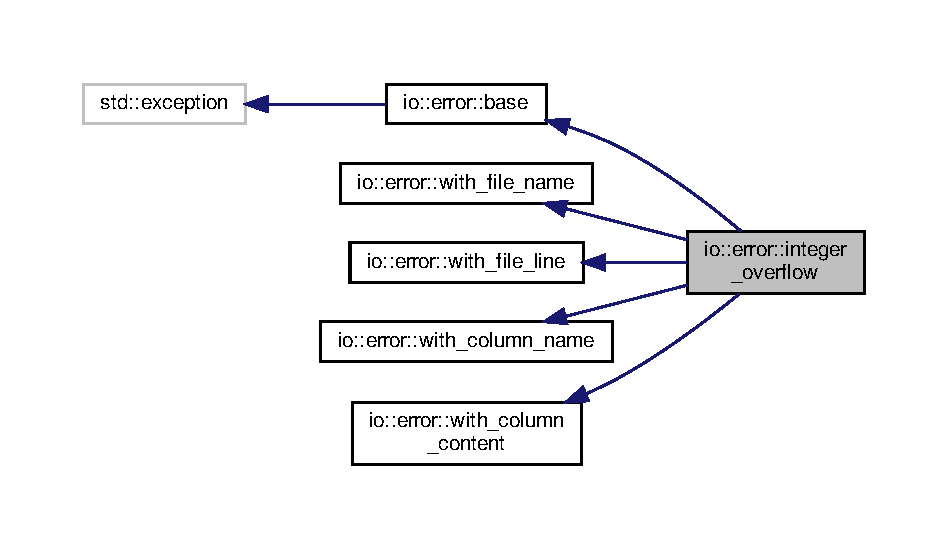
\includegraphics[width=350pt]{structio_1_1error_1_1integer__overflow__coll__graph}
\end{center}
\end{figure}
\subsection*{Public Member Functions}
\begin{DoxyCompactItemize}
\item 
\mbox{\Hypertarget{structio_1_1error_1_1integer__overflow_a25825600c3c29210160ba201519e6312}\label{structio_1_1error_1_1integer__overflow_a25825600c3c29210160ba201519e6312}} 
void {\bfseries format\+\_\+error\+\_\+message} () const
\end{DoxyCompactItemize}
\subsection*{Additional Inherited Members}


The documentation for this struct was generated from the following file\+:\begin{DoxyCompactItemize}
\item 
/home/emanuele/catkin\+\_\+ws/src/ros\+\_\+float/include/ros\+\_\+float/csv.\+h\end{DoxyCompactItemize}

\hypertarget{structio_1_1error_1_1integer__underflow}{}\section{io\+:\+:error\+:\+:integer\+\_\+underflow Struct Reference}
\label{structio_1_1error_1_1integer__underflow}\index{io\+::error\+::integer\+\_\+underflow@{io\+::error\+::integer\+\_\+underflow}}


Inheritance diagram for io\+:\+:error\+:\+:integer\+\_\+underflow\+:\nopagebreak
\begin{figure}[H]
\begin{center}
\leavevmode
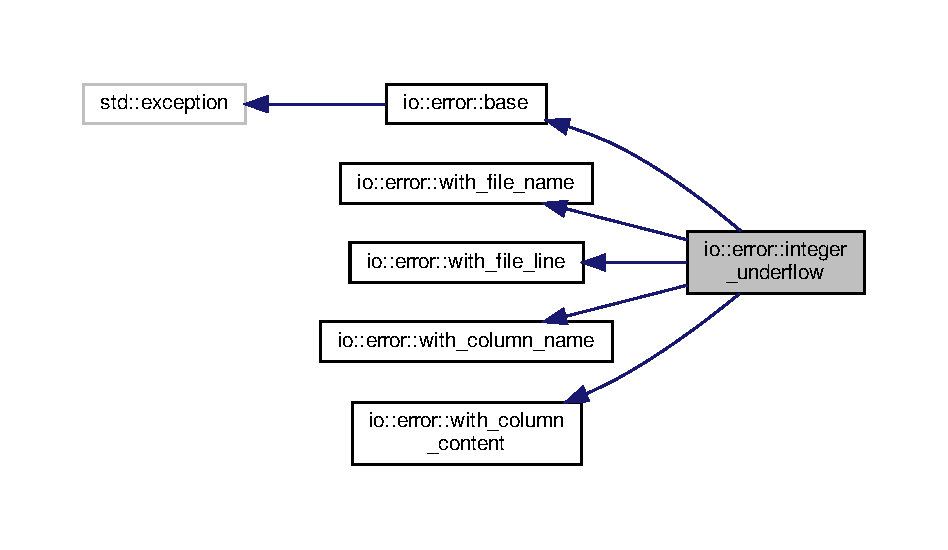
\includegraphics[width=350pt]{structio_1_1error_1_1integer__underflow__inherit__graph}
\end{center}
\end{figure}


Collaboration diagram for io\+:\+:error\+:\+:integer\+\_\+underflow\+:\nopagebreak
\begin{figure}[H]
\begin{center}
\leavevmode
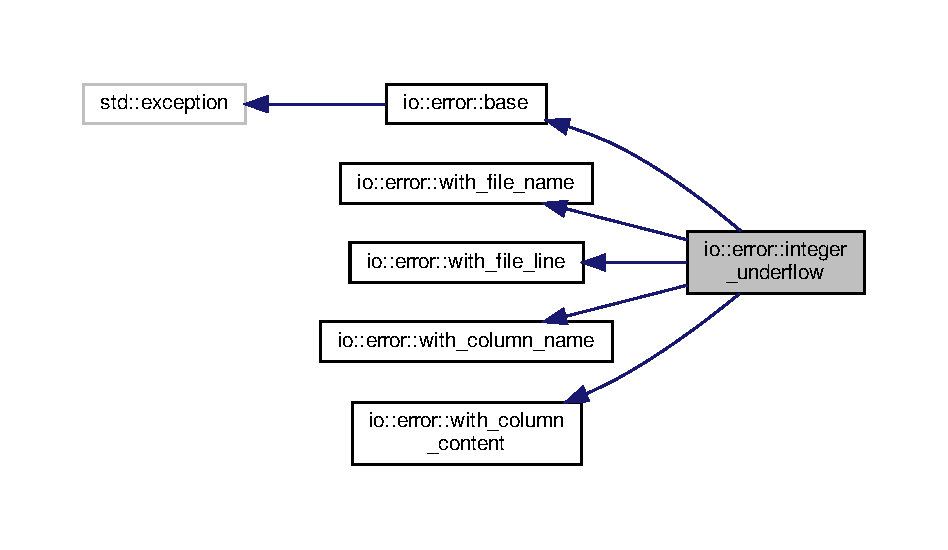
\includegraphics[width=350pt]{structio_1_1error_1_1integer__underflow__coll__graph}
\end{center}
\end{figure}
\subsection*{Public Member Functions}
\begin{DoxyCompactItemize}
\item 
\mbox{\Hypertarget{structio_1_1error_1_1integer__underflow_a2ded9c7e982403877055514543207847}\label{structio_1_1error_1_1integer__underflow_a2ded9c7e982403877055514543207847}} 
void {\bfseries format\+\_\+error\+\_\+message} () const
\end{DoxyCompactItemize}
\subsection*{Additional Inherited Members}


The documentation for this struct was generated from the following file\+:\begin{DoxyCompactItemize}
\item 
/home/emanuele/catkin\+\_\+ws/src/ros\+\_\+float/include/ros\+\_\+float/csv.\+h\end{DoxyCompactItemize}

\hypertarget{structio_1_1error_1_1invalid__single__character}{}\section{io\+:\+:error\+:\+:invalid\+\_\+single\+\_\+character Struct Reference}
\label{structio_1_1error_1_1invalid__single__character}\index{io\+::error\+::invalid\+\_\+single\+\_\+character@{io\+::error\+::invalid\+\_\+single\+\_\+character}}


Inheritance diagram for io\+:\+:error\+:\+:invalid\+\_\+single\+\_\+character\+:\nopagebreak
\begin{figure}[H]
\begin{center}
\leavevmode
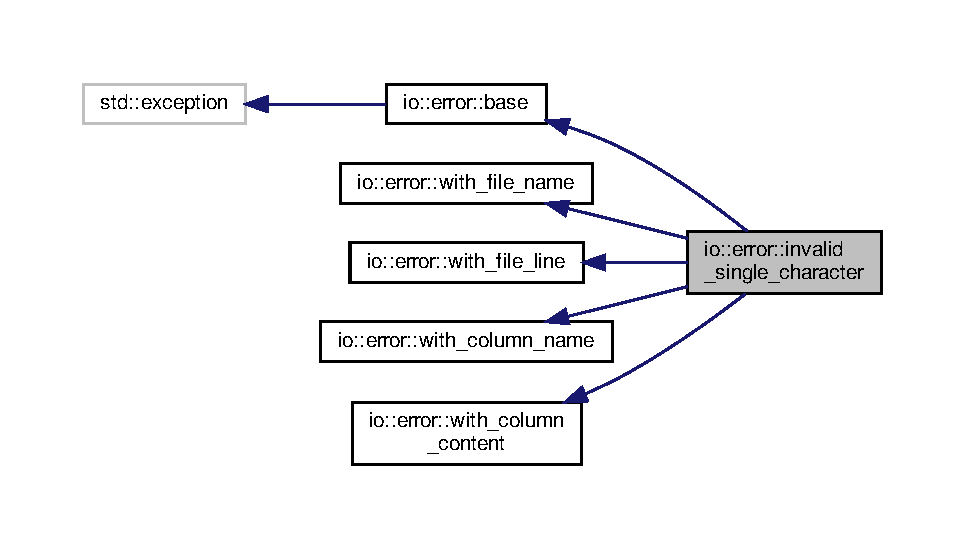
\includegraphics[width=350pt]{structio_1_1error_1_1invalid__single__character__inherit__graph}
\end{center}
\end{figure}


Collaboration diagram for io\+:\+:error\+:\+:invalid\+\_\+single\+\_\+character\+:\nopagebreak
\begin{figure}[H]
\begin{center}
\leavevmode
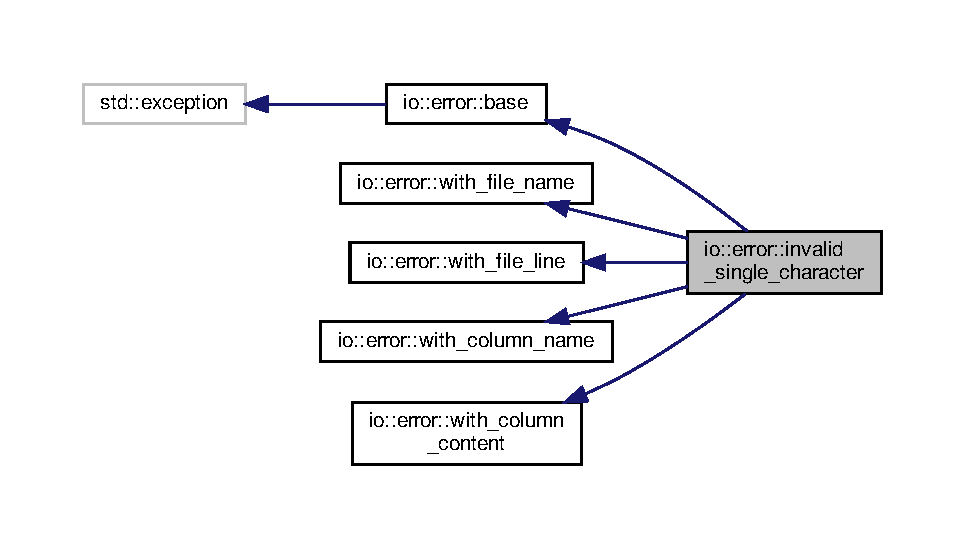
\includegraphics[width=350pt]{structio_1_1error_1_1invalid__single__character__coll__graph}
\end{center}
\end{figure}
\subsection*{Public Member Functions}
\begin{DoxyCompactItemize}
\item 
\mbox{\Hypertarget{structio_1_1error_1_1invalid__single__character_a074ab35a8013ad15041a9bb9188e69bf}\label{structio_1_1error_1_1invalid__single__character_a074ab35a8013ad15041a9bb9188e69bf}} 
void {\bfseries format\+\_\+error\+\_\+message} () const
\end{DoxyCompactItemize}
\subsection*{Additional Inherited Members}


The documentation for this struct was generated from the following file\+:\begin{DoxyCompactItemize}
\item 
/home/emanuele/catkin\+\_\+ws/src/ros\+\_\+float/include/ros\+\_\+float/csv.\+h\end{DoxyCompactItemize}

\hypertarget{structKELLER__DATA}{}\section{K\+E\+L\+L\+E\+R\+\_\+\+D\+A\+TA Struct Reference}
\label{structKELLER__DATA}\index{K\+E\+L\+L\+E\+R\+\_\+\+D\+A\+TA@{K\+E\+L\+L\+E\+R\+\_\+\+D\+A\+TA}}
\subsection*{Public Attributes}
\begin{DoxyCompactItemize}
\item 
\mbox{\Hypertarget{structKELLER__DATA_a3ba762f671afd7a08a999df8553fc17e}\label{structKELLER__DATA_a3ba762f671afd7a08a999df8553fc17e}} 
unsigned long {\bfseries timestamp}
\item 
\mbox{\Hypertarget{structKELLER__DATA_a146db119626551b896f98a959efe706d}\label{structKELLER__DATA_a146db119626551b896f98a959efe706d}} 
double {\bfseries depth}
\item 
\mbox{\Hypertarget{structKELLER__DATA_a19a08dde72e5c43f3bb85423f70b8baa}\label{structKELLER__DATA_a19a08dde72e5c43f3bb85423f70b8baa}} 
double {\bfseries temperature}
\item 
\mbox{\Hypertarget{structKELLER__DATA_ae65eb30765f03627278204e9da18c9b8}\label{structKELLER__DATA_ae65eb30765f03627278204e9da18c9b8}} 
double {\bfseries pressure}
\end{DoxyCompactItemize}


The documentation for this struct was generated from the following file\+:\begin{DoxyCompactItemize}
\item 
/home/emanuele/catkin\+\_\+ws/src/ros\+\_\+float/include/ros\+\_\+float/keller\+\_\+reader.\+h\end{DoxyCompactItemize}

\hypertarget{classKeller__reader}{}\section{Keller\+\_\+reader Class Reference}
\label{classKeller__reader}\index{Keller\+\_\+reader@{Keller\+\_\+reader}}


Collaboration diagram for Keller\+\_\+reader\+:\nopagebreak
\begin{figure}[H]
\begin{center}
\leavevmode
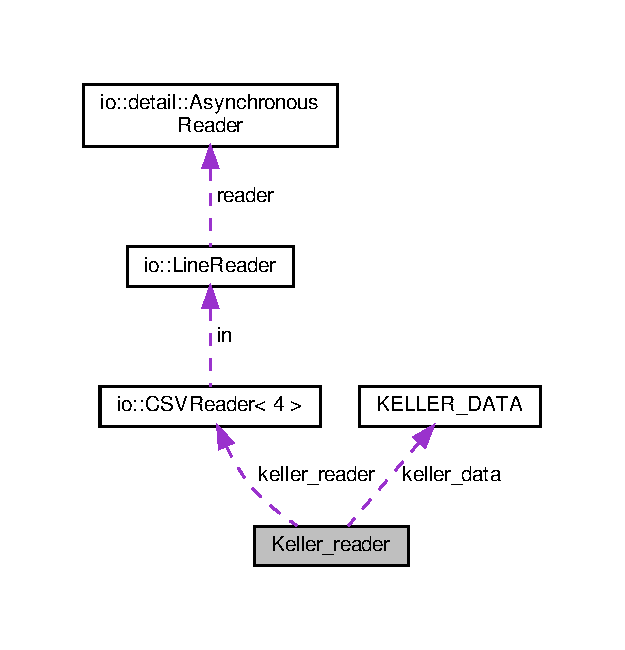
\includegraphics[width=300pt]{classKeller__reader__coll__graph}
\end{center}
\end{figure}
\subsection*{Public Member Functions}
\begin{DoxyCompactItemize}
\item 
\mbox{\Hypertarget{classKeller__reader_af02af436842fe2678d6589c3f1b146db}\label{classKeller__reader_af02af436842fe2678d6589c3f1b146db}} 
{\bfseries Keller\+\_\+reader} (std\+::string filename)
\item 
\mbox{\Hypertarget{classKeller__reader_ab77d4a9f47de55c6b8d891f08d662785}\label{classKeller__reader_ab77d4a9f47de55c6b8d891f08d662785}} 
bool {\bfseries next\+Line} ()
\end{DoxyCompactItemize}
\subsection*{Public Attributes}
\begin{DoxyCompactItemize}
\item 
\mbox{\Hypertarget{classKeller__reader_a2d73223c9cae72b889f1d121e2f629d5}\label{classKeller__reader_a2d73223c9cae72b889f1d121e2f629d5}} 
\hyperlink{structKELLER__DATA}{K\+E\+L\+L\+E\+R\+\_\+\+D\+A\+TA} {\bfseries keller\+\_\+data}
\item 
\mbox{\Hypertarget{classKeller__reader_a9c2c2985184a95c46f106c1e549340c0}\label{classKeller__reader_a9c2c2985184a95c46f106c1e549340c0}} 
sensor\+\_\+msgs\+::\+Fluid\+Pressure {\bfseries pressure\+Msg}
\item 
\mbox{\Hypertarget{classKeller__reader_a4ef560019ef100b52d6fd46b497a84eb}\label{classKeller__reader_a4ef560019ef100b52d6fd46b497a84eb}} 
ros\+\_\+float\+::pressure {\bfseries p\+Msg}
\item 
\mbox{\Hypertarget{classKeller__reader_aca76ed46c7e828e131c99df919dee597}\label{classKeller__reader_aca76ed46c7e828e131c99df919dee597}} 
ros\+\_\+float\+::temperature {\bfseries t\+Msg}
\item 
\mbox{\Hypertarget{classKeller__reader_a9216da4b4ba9d3aab90a8d59e9cd9d93}\label{classKeller__reader_a9216da4b4ba9d3aab90a8d59e9cd9d93}} 
ros\+\_\+float\+::depth {\bfseries d\+Msg}
\end{DoxyCompactItemize}
\subsection*{Private Member Functions}
\begin{DoxyCompactItemize}
\item 
\mbox{\Hypertarget{classKeller__reader_a1447efaa0ca4da10c05aadfed883a07d}\label{classKeller__reader_a1447efaa0ca4da10c05aadfed883a07d}} 
void {\bfseries pack\+Pressure\+Msg} ()
\item 
\mbox{\Hypertarget{classKeller__reader_a2c5b455f877fbca9ae2af0891991d948}\label{classKeller__reader_a2c5b455f877fbca9ae2af0891991d948}} 
void {\bfseries pack\+Custom\+\_\+\+Temperature\+Msg} ()
\item 
\mbox{\Hypertarget{classKeller__reader_aec80d676479ec7193b5070e57450bf32}\label{classKeller__reader_aec80d676479ec7193b5070e57450bf32}} 
void {\bfseries pack\+Custom\+\_\+\+Depth\+Msg} ()
\end{DoxyCompactItemize}
\subsection*{Private Attributes}
\begin{DoxyCompactItemize}
\item 
\mbox{\Hypertarget{classKeller__reader_a4fcf1b20e6a5fe8a262b12042ab433bd}\label{classKeller__reader_a4fcf1b20e6a5fe8a262b12042ab433bd}} 
\hyperlink{classio_1_1CSVReader}{io\+::\+C\+S\+V\+Reader}$<$ 4 $>$ {\bfseries keller\+\_\+reader}
\item 
\mbox{\Hypertarget{classKeller__reader_a09fb87959f1d7228d22ab26d6d858912}\label{classKeller__reader_a09fb87959f1d7228d22ab26d6d858912}} 
unsigned int {\bfseries msg\+Num\+Keller}
\end{DoxyCompactItemize}


The documentation for this class was generated from the following files\+:\begin{DoxyCompactItemize}
\item 
/home/emanuele/catkin\+\_\+ws/src/ros\+\_\+float/include/ros\+\_\+float/keller\+\_\+reader.\+h\item 
/home/emanuele/catkin\+\_\+ws/src/ros\+\_\+float/include/ros\+\_\+float/keller\+\_\+reader.\+cpp\end{DoxyCompactItemize}

\hypertarget{structio_1_1error_1_1line__length__limit__exceeded}{}\section{io\+:\+:error\+:\+:line\+\_\+length\+\_\+limit\+\_\+exceeded Struct Reference}
\label{structio_1_1error_1_1line__length__limit__exceeded}\index{io\+::error\+::line\+\_\+length\+\_\+limit\+\_\+exceeded@{io\+::error\+::line\+\_\+length\+\_\+limit\+\_\+exceeded}}


Inheritance diagram for io\+:\+:error\+:\+:line\+\_\+length\+\_\+limit\+\_\+exceeded\+:\nopagebreak
\begin{figure}[H]
\begin{center}
\leavevmode
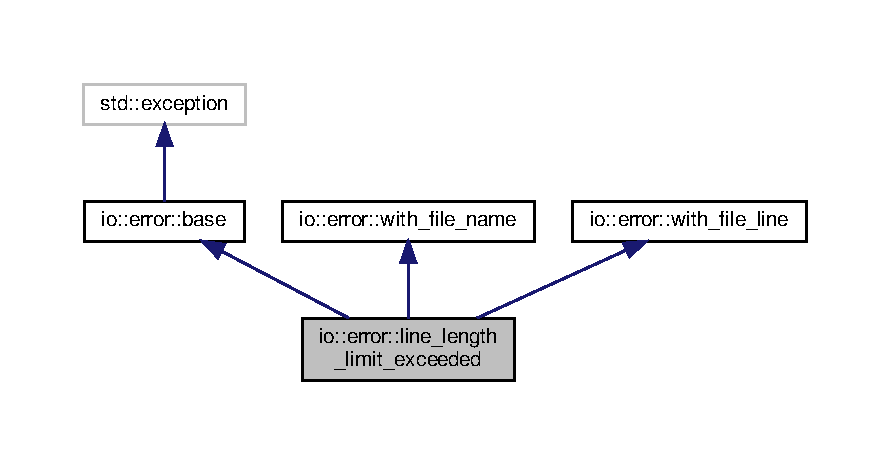
\includegraphics[width=350pt]{structio_1_1error_1_1line__length__limit__exceeded__inherit__graph}
\end{center}
\end{figure}


Collaboration diagram for io\+:\+:error\+:\+:line\+\_\+length\+\_\+limit\+\_\+exceeded\+:\nopagebreak
\begin{figure}[H]
\begin{center}
\leavevmode
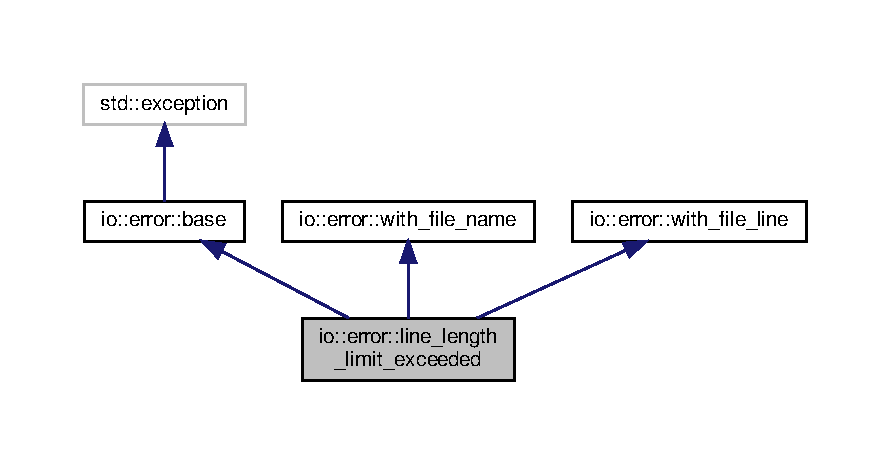
\includegraphics[width=350pt]{structio_1_1error_1_1line__length__limit__exceeded__coll__graph}
\end{center}
\end{figure}
\subsection*{Public Member Functions}
\begin{DoxyCompactItemize}
\item 
\mbox{\Hypertarget{structio_1_1error_1_1line__length__limit__exceeded_ae6ef1cf3ed1d82804953ac120892b85e}\label{structio_1_1error_1_1line__length__limit__exceeded_ae6ef1cf3ed1d82804953ac120892b85e}} 
void {\bfseries format\+\_\+error\+\_\+message} () const
\end{DoxyCompactItemize}
\subsection*{Additional Inherited Members}


The documentation for this struct was generated from the following file\+:\begin{DoxyCompactItemize}
\item 
/home/emanuele/catkin\+\_\+ws/src/ros\+\_\+float/include/ros\+\_\+float/csv.\+h\end{DoxyCompactItemize}

\hypertarget{classio_1_1LineReader}{}\section{io\+:\+:Line\+Reader Class Reference}
\label{classio_1_1LineReader}\index{io\+::\+Line\+Reader@{io\+::\+Line\+Reader}}


Collaboration diagram for io\+:\+:Line\+Reader\+:\nopagebreak
\begin{figure}[H]
\begin{center}
\leavevmode
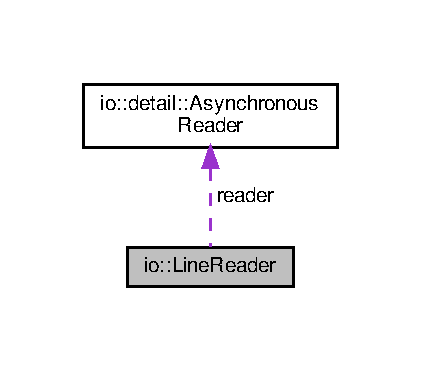
\includegraphics[width=202pt]{classio_1_1LineReader__coll__graph}
\end{center}
\end{figure}
\subsection*{Public Member Functions}
\begin{DoxyCompactItemize}
\item 
\mbox{\Hypertarget{classio_1_1LineReader_a84f2957de769bb701eaaddfd8bc004dd}\label{classio_1_1LineReader_a84f2957de769bb701eaaddfd8bc004dd}} 
{\bfseries Line\+Reader} (const \hyperlink{classio_1_1LineReader}{Line\+Reader} \&)=delete
\item 
\mbox{\Hypertarget{classio_1_1LineReader_a9ebd7beca16060ffc0ea8df3c0c6ff25}\label{classio_1_1LineReader_a9ebd7beca16060ffc0ea8df3c0c6ff25}} 
\hyperlink{classio_1_1LineReader}{Line\+Reader} \& {\bfseries operator=} (const \hyperlink{classio_1_1LineReader}{Line\+Reader} \&)=delete
\item 
\mbox{\Hypertarget{classio_1_1LineReader_a81a75d3f53725d35822f490007520e29}\label{classio_1_1LineReader_a81a75d3f53725d35822f490007520e29}} 
{\bfseries Line\+Reader} (const char $\ast$file\+\_\+name)
\item 
\mbox{\Hypertarget{classio_1_1LineReader_ab0eb26f44fa6b18f9c39dfb2561ac882}\label{classio_1_1LineReader_ab0eb26f44fa6b18f9c39dfb2561ac882}} 
{\bfseries Line\+Reader} (const std\+::string \&file\+\_\+name)
\item 
\mbox{\Hypertarget{classio_1_1LineReader_af4ebb130a7d6c78356573f6d0304266c}\label{classio_1_1LineReader_af4ebb130a7d6c78356573f6d0304266c}} 
{\bfseries Line\+Reader} (const char $\ast$file\+\_\+name, std\+::unique\+\_\+ptr$<$ \hyperlink{classio_1_1ByteSourceBase}{Byte\+Source\+Base} $>$byte\+\_\+source)
\item 
\mbox{\Hypertarget{classio_1_1LineReader_ab625b3a8001dca811b0e211c6cfc1b28}\label{classio_1_1LineReader_ab625b3a8001dca811b0e211c6cfc1b28}} 
{\bfseries Line\+Reader} (const std\+::string \&file\+\_\+name, std\+::unique\+\_\+ptr$<$ \hyperlink{classio_1_1ByteSourceBase}{Byte\+Source\+Base} $>$byte\+\_\+source)
\item 
\mbox{\Hypertarget{classio_1_1LineReader_ad5a65d6f23474884061a77ea858c042b}\label{classio_1_1LineReader_ad5a65d6f23474884061a77ea858c042b}} 
{\bfseries Line\+Reader} (const char $\ast$file\+\_\+name, const char $\ast$data\+\_\+begin, const char $\ast$data\+\_\+end)
\item 
\mbox{\Hypertarget{classio_1_1LineReader_a0a52d864b46442a253443cac1367366e}\label{classio_1_1LineReader_a0a52d864b46442a253443cac1367366e}} 
{\bfseries Line\+Reader} (const std\+::string \&file\+\_\+name, const char $\ast$data\+\_\+begin, const char $\ast$data\+\_\+end)
\item 
\mbox{\Hypertarget{classio_1_1LineReader_ad2a8943ba0848ae5052e2f5ad30c010e}\label{classio_1_1LineReader_ad2a8943ba0848ae5052e2f5ad30c010e}} 
{\bfseries Line\+Reader} (const char $\ast$file\+\_\+name, F\+I\+LE $\ast$file)
\item 
\mbox{\Hypertarget{classio_1_1LineReader_a93fa2e3ae98b0e7a7391714d6395c552}\label{classio_1_1LineReader_a93fa2e3ae98b0e7a7391714d6395c552}} 
{\bfseries Line\+Reader} (const std\+::string \&file\+\_\+name, F\+I\+LE $\ast$file)
\item 
\mbox{\Hypertarget{classio_1_1LineReader_a301c08eb9ca5d3fdccf4e9a8e5ac82f8}\label{classio_1_1LineReader_a301c08eb9ca5d3fdccf4e9a8e5ac82f8}} 
{\bfseries Line\+Reader} (const char $\ast$file\+\_\+name, std\+::istream \&in)
\item 
\mbox{\Hypertarget{classio_1_1LineReader_a3eacf4d1539a24122c6897fce4e72f06}\label{classio_1_1LineReader_a3eacf4d1539a24122c6897fce4e72f06}} 
{\bfseries Line\+Reader} (const std\+::string \&file\+\_\+name, std\+::istream \&in)
\item 
\mbox{\Hypertarget{classio_1_1LineReader_a1a0763d491dec16cebc33134e965dfee}\label{classio_1_1LineReader_a1a0763d491dec16cebc33134e965dfee}} 
void {\bfseries set\+\_\+file\+\_\+name} (const std\+::string \&file\+\_\+name)
\item 
\mbox{\Hypertarget{classio_1_1LineReader_a81c56ac68497da5ec874333ce063fd83}\label{classio_1_1LineReader_a81c56ac68497da5ec874333ce063fd83}} 
void {\bfseries set\+\_\+file\+\_\+name} (const char $\ast$file\+\_\+name)
\item 
\mbox{\Hypertarget{classio_1_1LineReader_ad5817da6af1ae77daddec7aeaeebf2f8}\label{classio_1_1LineReader_ad5817da6af1ae77daddec7aeaeebf2f8}} 
const char $\ast$ {\bfseries get\+\_\+truncated\+\_\+file\+\_\+name} () const
\item 
\mbox{\Hypertarget{classio_1_1LineReader_a581b55d4ced6adb964de50fa8ac6eb08}\label{classio_1_1LineReader_a581b55d4ced6adb964de50fa8ac6eb08}} 
void {\bfseries set\+\_\+file\+\_\+line} (unsigned file\+\_\+line)
\item 
\mbox{\Hypertarget{classio_1_1LineReader_a3f3459e22ed8e459238c290050b6722e}\label{classio_1_1LineReader_a3f3459e22ed8e459238c290050b6722e}} 
unsigned {\bfseries get\+\_\+file\+\_\+line} () const
\item 
\mbox{\Hypertarget{classio_1_1LineReader_a97f4e0129611d9da2b8c966ffe670be5}\label{classio_1_1LineReader_a97f4e0129611d9da2b8c966ffe670be5}} 
char $\ast$ {\bfseries next\+\_\+line} ()
\end{DoxyCompactItemize}
\subsection*{Private Member Functions}
\begin{DoxyCompactItemize}
\item 
\mbox{\Hypertarget{classio_1_1LineReader_a68ac92cedd46d25cbc4e205eb3a2833f}\label{classio_1_1LineReader_a68ac92cedd46d25cbc4e205eb3a2833f}} 
void {\bfseries init} (std\+::unique\+\_\+ptr$<$ \hyperlink{classio_1_1ByteSourceBase}{Byte\+Source\+Base} $>$byte\+\_\+source)
\end{DoxyCompactItemize}
\subsection*{Static Private Member Functions}
\begin{DoxyCompactItemize}
\item 
\mbox{\Hypertarget{classio_1_1LineReader_a036adce726096bca1db7ccceea938595}\label{classio_1_1LineReader_a036adce726096bca1db7ccceea938595}} 
static std\+::unique\+\_\+ptr$<$ \hyperlink{classio_1_1ByteSourceBase}{Byte\+Source\+Base} $>$ {\bfseries open\+\_\+file} (const char $\ast$file\+\_\+name)
\end{DoxyCompactItemize}
\subsection*{Private Attributes}
\begin{DoxyCompactItemize}
\item 
\mbox{\Hypertarget{classio_1_1LineReader_afd45c8f7175a4094a469f5764816d181}\label{classio_1_1LineReader_afd45c8f7175a4094a469f5764816d181}} 
std\+::unique\+\_\+ptr$<$ char\mbox{[}$\,$\mbox{]}$>$ {\bfseries buffer}
\item 
\mbox{\Hypertarget{classio_1_1LineReader_abfd04ef491b6515a26b1b17aab9430b0}\label{classio_1_1LineReader_abfd04ef491b6515a26b1b17aab9430b0}} 
\hyperlink{classio_1_1detail_1_1AsynchronousReader}{detail\+::\+Asynchronous\+Reader} {\bfseries reader}
\item 
\mbox{\Hypertarget{classio_1_1LineReader_a20676a014d14bfa566591d8cfeed0f29}\label{classio_1_1LineReader_a20676a014d14bfa566591d8cfeed0f29}} 
int {\bfseries data\+\_\+begin}
\item 
\mbox{\Hypertarget{classio_1_1LineReader_a16829b470aa908981d4799401d42a85b}\label{classio_1_1LineReader_a16829b470aa908981d4799401d42a85b}} 
int {\bfseries data\+\_\+end}
\item 
\mbox{\Hypertarget{classio_1_1LineReader_a8b853ac45c1eae0afc36d49630e949d8}\label{classio_1_1LineReader_a8b853ac45c1eae0afc36d49630e949d8}} 
char {\bfseries file\+\_\+name} \mbox{[}error\+::max\+\_\+file\+\_\+name\+\_\+length+1\mbox{]}
\item 
\mbox{\Hypertarget{classio_1_1LineReader_a5c29ad60208bca6475af54e54eff80b7}\label{classio_1_1LineReader_a5c29ad60208bca6475af54e54eff80b7}} 
unsigned {\bfseries file\+\_\+line}
\end{DoxyCompactItemize}
\subsection*{Static Private Attributes}
\begin{DoxyCompactItemize}
\item 
\mbox{\Hypertarget{classio_1_1LineReader_a04db9ad3b956347b48136dbe5751469d}\label{classio_1_1LineReader_a04db9ad3b956347b48136dbe5751469d}} 
static const int {\bfseries block\+\_\+len} = 1$<$$<$24
\end{DoxyCompactItemize}


The documentation for this class was generated from the following file\+:\begin{DoxyCompactItemize}
\item 
/home/emanuele/catkin\+\_\+ws/src/ros\+\_\+float/include/ros\+\_\+float/csv.\+h\end{DoxyCompactItemize}

\hypertarget{structio_1_1error_1_1missing__column__in__header}{}\section{io\+:\+:error\+:\+:missing\+\_\+column\+\_\+in\+\_\+header Struct Reference}
\label{structio_1_1error_1_1missing__column__in__header}\index{io\+::error\+::missing\+\_\+column\+\_\+in\+\_\+header@{io\+::error\+::missing\+\_\+column\+\_\+in\+\_\+header}}


Inheritance diagram for io\+:\+:error\+:\+:missing\+\_\+column\+\_\+in\+\_\+header\+:\nopagebreak
\begin{figure}[H]
\begin{center}
\leavevmode
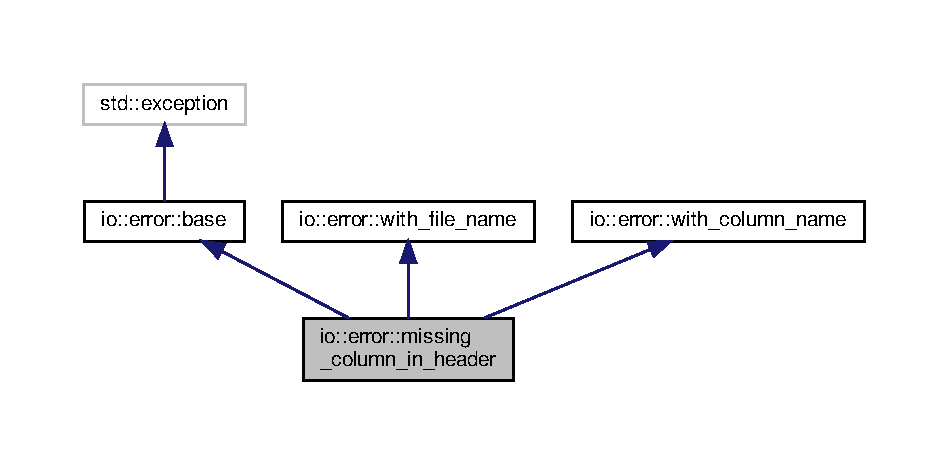
\includegraphics[width=350pt]{structio_1_1error_1_1missing__column__in__header__inherit__graph}
\end{center}
\end{figure}


Collaboration diagram for io\+:\+:error\+:\+:missing\+\_\+column\+\_\+in\+\_\+header\+:\nopagebreak
\begin{figure}[H]
\begin{center}
\leavevmode
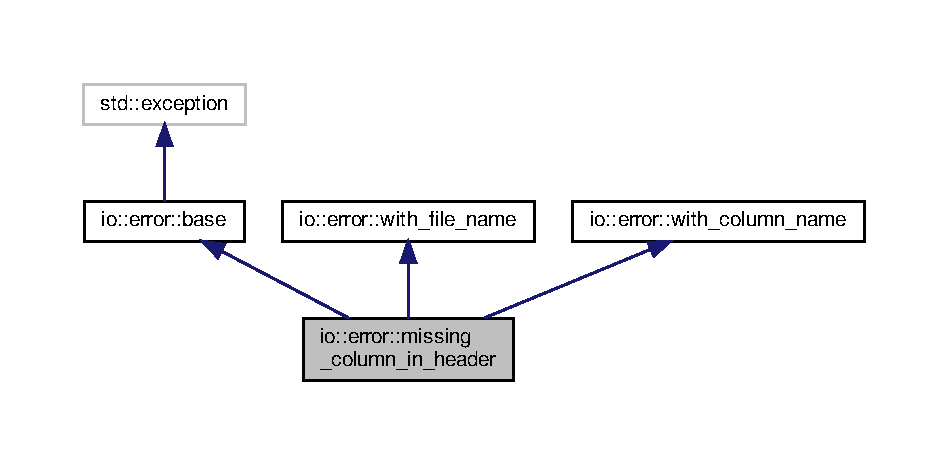
\includegraphics[width=350pt]{structio_1_1error_1_1missing__column__in__header__coll__graph}
\end{center}
\end{figure}
\subsection*{Public Member Functions}
\begin{DoxyCompactItemize}
\item 
\mbox{\Hypertarget{structio_1_1error_1_1missing__column__in__header_a1a2bd4e01a389cb50c6bfae8443317fd}\label{structio_1_1error_1_1missing__column__in__header_a1a2bd4e01a389cb50c6bfae8443317fd}} 
void {\bfseries format\+\_\+error\+\_\+message} () const
\end{DoxyCompactItemize}
\subsection*{Additional Inherited Members}


The documentation for this struct was generated from the following file\+:\begin{DoxyCompactItemize}
\item 
/home/emanuele/catkin\+\_\+ws/src/ros\+\_\+float/include/ros\+\_\+float/csv.\+h\end{DoxyCompactItemize}

\hypertarget{structio_1_1no__comment}{}\section{io\+:\+:no\+\_\+comment Struct Reference}
\label{structio_1_1no__comment}\index{io\+::no\+\_\+comment@{io\+::no\+\_\+comment}}
\subsection*{Static Public Member Functions}
\begin{DoxyCompactItemize}
\item 
\mbox{\Hypertarget{structio_1_1no__comment_a52b252547482e28edd076ee2224bc8d8}\label{structio_1_1no__comment_a52b252547482e28edd076ee2224bc8d8}} 
static bool {\bfseries is\+\_\+comment} (const char $\ast$)
\end{DoxyCompactItemize}


The documentation for this struct was generated from the following file\+:\begin{DoxyCompactItemize}
\item 
/home/emanuele/catkin\+\_\+ws/src/ros\+\_\+float/include/ros\+\_\+float/csv.\+h\end{DoxyCompactItemize}

\hypertarget{structio_1_1error_1_1no__digit}{}\section{io\+:\+:error\+:\+:no\+\_\+digit Struct Reference}
\label{structio_1_1error_1_1no__digit}\index{io\+::error\+::no\+\_\+digit@{io\+::error\+::no\+\_\+digit}}


Inheritance diagram for io\+:\+:error\+:\+:no\+\_\+digit\+:\nopagebreak
\begin{figure}[H]
\begin{center}
\leavevmode
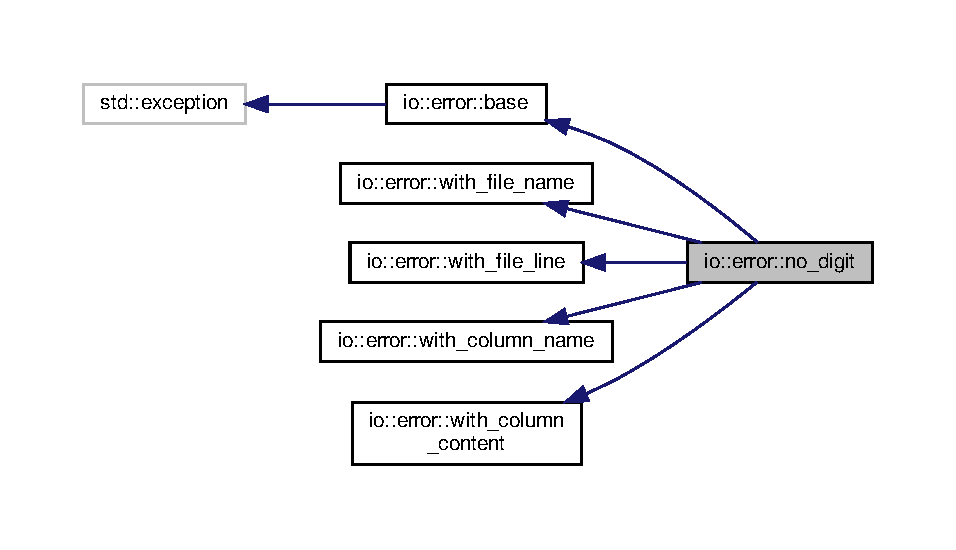
\includegraphics[width=350pt]{structio_1_1error_1_1no__digit__inherit__graph}
\end{center}
\end{figure}


Collaboration diagram for io\+:\+:error\+:\+:no\+\_\+digit\+:\nopagebreak
\begin{figure}[H]
\begin{center}
\leavevmode
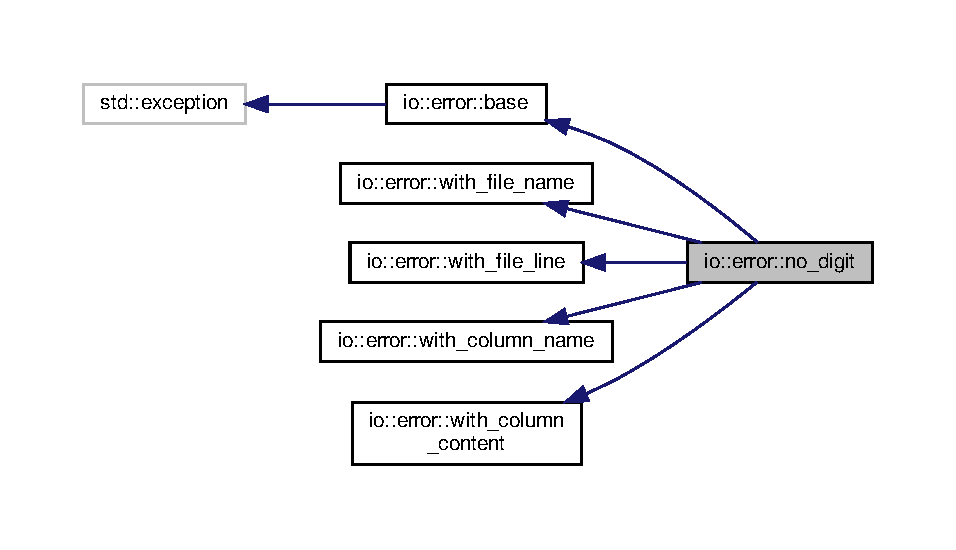
\includegraphics[width=350pt]{structio_1_1error_1_1no__digit__coll__graph}
\end{center}
\end{figure}
\subsection*{Public Member Functions}
\begin{DoxyCompactItemize}
\item 
\mbox{\Hypertarget{structio_1_1error_1_1no__digit_a469275c63f67171903f9cdb2418da5b3}\label{structio_1_1error_1_1no__digit_a469275c63f67171903f9cdb2418da5b3}} 
void {\bfseries format\+\_\+error\+\_\+message} () const
\end{DoxyCompactItemize}
\subsection*{Additional Inherited Members}


The documentation for this struct was generated from the following file\+:\begin{DoxyCompactItemize}
\item 
/home/emanuele/catkin\+\_\+ws/src/ros\+\_\+float/include/ros\+\_\+float/csv.\+h\end{DoxyCompactItemize}

\hypertarget{structio_1_1no__quote__escape}{}\section{io\+:\+:no\+\_\+quote\+\_\+escape$<$ sep $>$ Struct Template Reference}
\label{structio_1_1no__quote__escape}\index{io\+::no\+\_\+quote\+\_\+escape$<$ sep $>$@{io\+::no\+\_\+quote\+\_\+escape$<$ sep $>$}}
\subsection*{Static Public Member Functions}
\begin{DoxyCompactItemize}
\item 
\mbox{\Hypertarget{structio_1_1no__quote__escape_add17b043bb89445079a0448026ce86d0}\label{structio_1_1no__quote__escape_add17b043bb89445079a0448026ce86d0}} 
static const char $\ast$ {\bfseries find\+\_\+next\+\_\+column\+\_\+end} (const char $\ast$col\+\_\+begin)
\item 
\mbox{\Hypertarget{structio_1_1no__quote__escape_af1c217f2c995d178a91c58235191b052}\label{structio_1_1no__quote__escape_af1c217f2c995d178a91c58235191b052}} 
static void {\bfseries unescape} (char $\ast$\&, char $\ast$\&)
\end{DoxyCompactItemize}


The documentation for this struct was generated from the following file\+:\begin{DoxyCompactItemize}
\item 
/home/emanuele/catkin\+\_\+ws/src/ros\+\_\+float/include/ros\+\_\+float/csv.\+h\end{DoxyCompactItemize}

\hypertarget{classio_1_1detail_1_1NonOwningIStreamByteSource}{}\section{io\+:\+:detail\+:\+:Non\+Owning\+I\+Stream\+Byte\+Source Class Reference}
\label{classio_1_1detail_1_1NonOwningIStreamByteSource}\index{io\+::detail\+::\+Non\+Owning\+I\+Stream\+Byte\+Source@{io\+::detail\+::\+Non\+Owning\+I\+Stream\+Byte\+Source}}


Inheritance diagram for io\+:\+:detail\+:\+:Non\+Owning\+I\+Stream\+Byte\+Source\+:\nopagebreak
\begin{figure}[H]
\begin{center}
\leavevmode
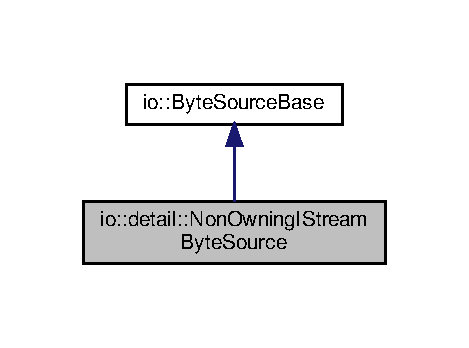
\includegraphics[width=225pt]{classio_1_1detail_1_1NonOwningIStreamByteSource__inherit__graph}
\end{center}
\end{figure}


Collaboration diagram for io\+:\+:detail\+:\+:Non\+Owning\+I\+Stream\+Byte\+Source\+:\nopagebreak
\begin{figure}[H]
\begin{center}
\leavevmode
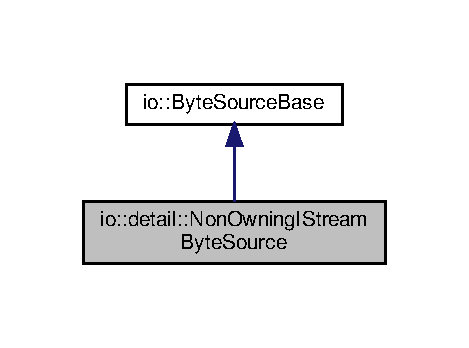
\includegraphics[width=225pt]{classio_1_1detail_1_1NonOwningIStreamByteSource__coll__graph}
\end{center}
\end{figure}
\subsection*{Public Member Functions}
\begin{DoxyCompactItemize}
\item 
\mbox{\Hypertarget{classio_1_1detail_1_1NonOwningIStreamByteSource_aacb55ba2f52ba1c30810697d6aa92169}\label{classio_1_1detail_1_1NonOwningIStreamByteSource_aacb55ba2f52ba1c30810697d6aa92169}} 
{\bfseries Non\+Owning\+I\+Stream\+Byte\+Source} (std\+::istream \&in)
\item 
\mbox{\Hypertarget{classio_1_1detail_1_1NonOwningIStreamByteSource_ac7b1968c8314896d7ec0ebb97fdda30d}\label{classio_1_1detail_1_1NonOwningIStreamByteSource_ac7b1968c8314896d7ec0ebb97fdda30d}} 
int {\bfseries read} (char $\ast$buffer, int size)
\end{DoxyCompactItemize}
\subsection*{Private Attributes}
\begin{DoxyCompactItemize}
\item 
\mbox{\Hypertarget{classio_1_1detail_1_1NonOwningIStreamByteSource_a42ec07be9409b77a17bdf08cfa73739d}\label{classio_1_1detail_1_1NonOwningIStreamByteSource_a42ec07be9409b77a17bdf08cfa73739d}} 
std\+::istream \& {\bfseries in}
\end{DoxyCompactItemize}


The documentation for this class was generated from the following file\+:\begin{DoxyCompactItemize}
\item 
/home/emanuele/catkin\+\_\+ws/src/ros\+\_\+float/include/ros\+\_\+float/csv.\+h\end{DoxyCompactItemize}

\hypertarget{classio_1_1detail_1_1NonOwningStringByteSource}{}\section{io\+:\+:detail\+:\+:Non\+Owning\+String\+Byte\+Source Class Reference}
\label{classio_1_1detail_1_1NonOwningStringByteSource}\index{io\+::detail\+::\+Non\+Owning\+String\+Byte\+Source@{io\+::detail\+::\+Non\+Owning\+String\+Byte\+Source}}


Inheritance diagram for io\+:\+:detail\+:\+:Non\+Owning\+String\+Byte\+Source\+:\nopagebreak
\begin{figure}[H]
\begin{center}
\leavevmode
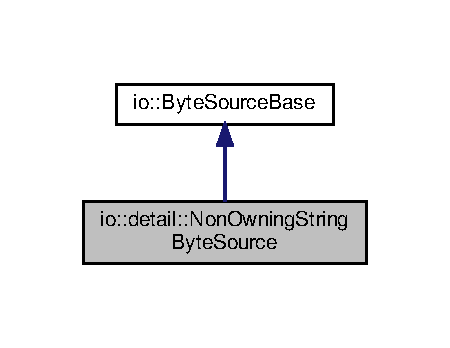
\includegraphics[width=216pt]{classio_1_1detail_1_1NonOwningStringByteSource__inherit__graph}
\end{center}
\end{figure}


Collaboration diagram for io\+:\+:detail\+:\+:Non\+Owning\+String\+Byte\+Source\+:\nopagebreak
\begin{figure}[H]
\begin{center}
\leavevmode
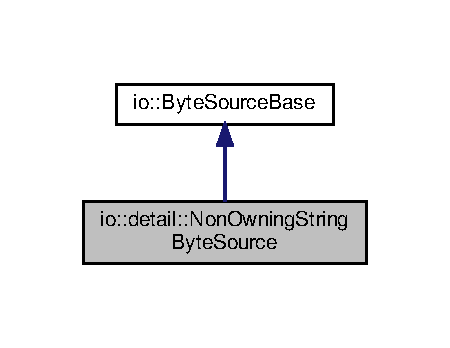
\includegraphics[width=216pt]{classio_1_1detail_1_1NonOwningStringByteSource__coll__graph}
\end{center}
\end{figure}
\subsection*{Public Member Functions}
\begin{DoxyCompactItemize}
\item 
\mbox{\Hypertarget{classio_1_1detail_1_1NonOwningStringByteSource_a8fd604017b38e20f90386b6e10bd95a3}\label{classio_1_1detail_1_1NonOwningStringByteSource_a8fd604017b38e20f90386b6e10bd95a3}} 
{\bfseries Non\+Owning\+String\+Byte\+Source} (const char $\ast$str, long long size)
\item 
\mbox{\Hypertarget{classio_1_1detail_1_1NonOwningStringByteSource_aba194be7e3a141f40d683db483a620bb}\label{classio_1_1detail_1_1NonOwningStringByteSource_aba194be7e3a141f40d683db483a620bb}} 
int {\bfseries read} (char $\ast$buffer, int desired\+\_\+byte\+\_\+count)
\end{DoxyCompactItemize}
\subsection*{Private Attributes}
\begin{DoxyCompactItemize}
\item 
\mbox{\Hypertarget{classio_1_1detail_1_1NonOwningStringByteSource_ad130b4796eb5758c3e512d585af51bef}\label{classio_1_1detail_1_1NonOwningStringByteSource_ad130b4796eb5758c3e512d585af51bef}} 
const char $\ast$ {\bfseries str}
\item 
\mbox{\Hypertarget{classio_1_1detail_1_1NonOwningStringByteSource_aa2097ba0c3c49f0266ec1fbc8f322947}\label{classio_1_1detail_1_1NonOwningStringByteSource_aa2097ba0c3c49f0266ec1fbc8f322947}} 
long long {\bfseries remaining\+\_\+byte\+\_\+count}
\end{DoxyCompactItemize}


The documentation for this class was generated from the following file\+:\begin{DoxyCompactItemize}
\item 
/home/emanuele/catkin\+\_\+ws/src/ros\+\_\+float/include/ros\+\_\+float/csv.\+h\end{DoxyCompactItemize}

\hypertarget{classio_1_1detail_1_1OwningStdIOByteSourceBase}{}\section{io\+:\+:detail\+:\+:Owning\+Std\+I\+O\+Byte\+Source\+Base Class Reference}
\label{classio_1_1detail_1_1OwningStdIOByteSourceBase}\index{io\+::detail\+::\+Owning\+Std\+I\+O\+Byte\+Source\+Base@{io\+::detail\+::\+Owning\+Std\+I\+O\+Byte\+Source\+Base}}


Inheritance diagram for io\+:\+:detail\+:\+:Owning\+Std\+I\+O\+Byte\+Source\+Base\+:\nopagebreak
\begin{figure}[H]
\begin{center}
\leavevmode
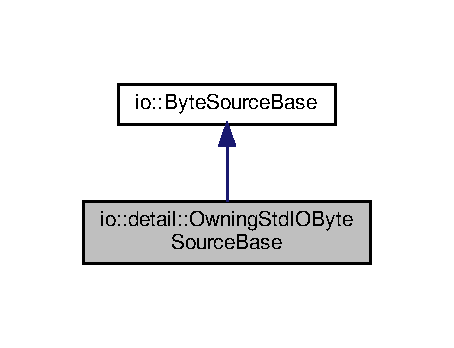
\includegraphics[width=218pt]{classio_1_1detail_1_1OwningStdIOByteSourceBase__inherit__graph}
\end{center}
\end{figure}


Collaboration diagram for io\+:\+:detail\+:\+:Owning\+Std\+I\+O\+Byte\+Source\+Base\+:\nopagebreak
\begin{figure}[H]
\begin{center}
\leavevmode
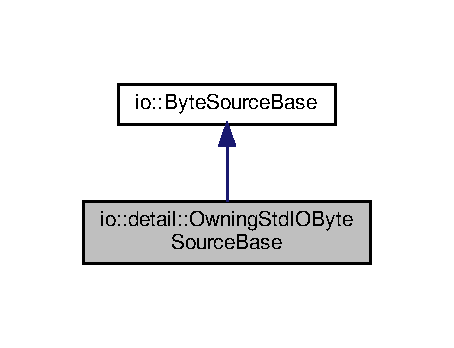
\includegraphics[width=218pt]{classio_1_1detail_1_1OwningStdIOByteSourceBase__coll__graph}
\end{center}
\end{figure}
\subsection*{Public Member Functions}
\begin{DoxyCompactItemize}
\item 
\mbox{\Hypertarget{classio_1_1detail_1_1OwningStdIOByteSourceBase_a259f77d1a3c57720b54b88d9f8a3c018}\label{classio_1_1detail_1_1OwningStdIOByteSourceBase_a259f77d1a3c57720b54b88d9f8a3c018}} 
{\bfseries Owning\+Std\+I\+O\+Byte\+Source\+Base} (F\+I\+LE $\ast$file)
\item 
\mbox{\Hypertarget{classio_1_1detail_1_1OwningStdIOByteSourceBase_a9269e7bfd07ebf2fa3518912fe7bebd0}\label{classio_1_1detail_1_1OwningStdIOByteSourceBase_a9269e7bfd07ebf2fa3518912fe7bebd0}} 
int {\bfseries read} (char $\ast$buffer, int size)
\end{DoxyCompactItemize}
\subsection*{Private Attributes}
\begin{DoxyCompactItemize}
\item 
\mbox{\Hypertarget{classio_1_1detail_1_1OwningStdIOByteSourceBase_a00f62c8522d0fe9edadf3d094e94ae26}\label{classio_1_1detail_1_1OwningStdIOByteSourceBase_a00f62c8522d0fe9edadf3d094e94ae26}} 
F\+I\+LE $\ast$ {\bfseries file}
\end{DoxyCompactItemize}


The documentation for this class was generated from the following file\+:\begin{DoxyCompactItemize}
\item 
/home/emanuele/catkin\+\_\+ws/src/ros\+\_\+float/include/ros\+\_\+float/csv.\+h\end{DoxyCompactItemize}

\hypertarget{structio_1_1set__to__max__on__overflow}{}\section{io\+:\+:set\+\_\+to\+\_\+max\+\_\+on\+\_\+overflow Struct Reference}
\label{structio_1_1set__to__max__on__overflow}\index{io\+::set\+\_\+to\+\_\+max\+\_\+on\+\_\+overflow@{io\+::set\+\_\+to\+\_\+max\+\_\+on\+\_\+overflow}}
\subsection*{Static Public Member Functions}
\begin{DoxyCompactItemize}
\item 
\mbox{\Hypertarget{structio_1_1set__to__max__on__overflow_a770dee97a1ee55131163e6be8d4c0d9d}\label{structio_1_1set__to__max__on__overflow_a770dee97a1ee55131163e6be8d4c0d9d}} 
{\footnotesize template$<$class T $>$ }\\static void {\bfseries on\+\_\+overflow} (T \&x)
\item 
\mbox{\Hypertarget{structio_1_1set__to__max__on__overflow_a812d316e2b23247df19ca83bfda90a59}\label{structio_1_1set__to__max__on__overflow_a812d316e2b23247df19ca83bfda90a59}} 
{\footnotesize template$<$class T $>$ }\\static void {\bfseries on\+\_\+underflow} (T \&x)
\end{DoxyCompactItemize}


The documentation for this struct was generated from the following file\+:\begin{DoxyCompactItemize}
\item 
/home/emanuele/catkin\+\_\+ws/src/ros\+\_\+float/include/ros\+\_\+float/csv.\+h\end{DoxyCompactItemize}

\hypertarget{classsimulationParser}{}\section{simulation\+Parser Class Reference}
\label{classsimulationParser}\index{simulation\+Parser@{simulation\+Parser}}


The documentation for this class was generated from the following files\+:\begin{DoxyCompactItemize}
\item 
/home/emanuele/catkin\+\_\+ws/src/ros\+\_\+float/include/ros\+\_\+float/simulationparser.\+h\item 
/home/emanuele/catkin\+\_\+ws/src/ros\+\_\+float/include/ros\+\_\+float/simulationparser.\+cpp\end{DoxyCompactItemize}

\hypertarget{structio_1_1single__and__empty__line__comment}{}\section{io\+:\+:single\+\_\+and\+\_\+empty\+\_\+line\+\_\+comment$<$ comment\+\_\+start\+\_\+char\+\_\+list $>$ Struct Template Reference}
\label{structio_1_1single__and__empty__line__comment}\index{io\+::single\+\_\+and\+\_\+empty\+\_\+line\+\_\+comment$<$ comment\+\_\+start\+\_\+char\+\_\+list $>$@{io\+::single\+\_\+and\+\_\+empty\+\_\+line\+\_\+comment$<$ comment\+\_\+start\+\_\+char\+\_\+list $>$}}
\subsection*{Static Public Member Functions}
\begin{DoxyCompactItemize}
\item 
\mbox{\Hypertarget{structio_1_1single__and__empty__line__comment_a93a1556dfe4d7e6e3a674d576c4b30f4}\label{structio_1_1single__and__empty__line__comment_a93a1556dfe4d7e6e3a674d576c4b30f4}} 
static bool {\bfseries is\+\_\+comment} (const char $\ast$line)
\end{DoxyCompactItemize}


The documentation for this struct was generated from the following file\+:\begin{DoxyCompactItemize}
\item 
/home/emanuele/catkin\+\_\+ws/src/ros\+\_\+float/include/ros\+\_\+float/csv.\+h\end{DoxyCompactItemize}

\hypertarget{structio_1_1single__line__comment}{}\section{io\+:\+:single\+\_\+line\+\_\+comment$<$ comment\+\_\+start\+\_\+char\+\_\+list $>$ Struct Template Reference}
\label{structio_1_1single__line__comment}\index{io\+::single\+\_\+line\+\_\+comment$<$ comment\+\_\+start\+\_\+char\+\_\+list $>$@{io\+::single\+\_\+line\+\_\+comment$<$ comment\+\_\+start\+\_\+char\+\_\+list $>$}}
\subsection*{Static Public Member Functions}
\begin{DoxyCompactItemize}
\item 
\mbox{\Hypertarget{structio_1_1single__line__comment_ac4b029bb0efd251505f8e610cc308a92}\label{structio_1_1single__line__comment_ac4b029bb0efd251505f8e610cc308a92}} 
static bool {\bfseries is\+\_\+comment} (const char $\ast$line)
\end{DoxyCompactItemize}
\subsection*{Static Private Member Functions}
\begin{DoxyCompactItemize}
\item 
\mbox{\Hypertarget{structio_1_1single__line__comment_a961a1b5c85dd2ec717ff483cb2206ade}\label{structio_1_1single__line__comment_a961a1b5c85dd2ec717ff483cb2206ade}} 
static constexpr bool {\bfseries is\+\_\+comment\+\_\+start\+\_\+char} (char)
\item 
\mbox{\Hypertarget{structio_1_1single__line__comment_a9533453f729d2216f52af087e4411548}\label{structio_1_1single__line__comment_a9533453f729d2216f52af087e4411548}} 
{\footnotesize template$<$class ... Other\+Comment\+Start\+Chars$>$ }\\static constexpr bool {\bfseries is\+\_\+comment\+\_\+start\+\_\+char} (char c, char comment\+\_\+start\+\_\+char, Other\+Comment\+Start\+Chars...\+other\+\_\+comment\+\_\+start\+\_\+chars)
\end{DoxyCompactItemize}


The documentation for this struct was generated from the following file\+:\begin{DoxyCompactItemize}
\item 
/home/emanuele/catkin\+\_\+ws/src/ros\+\_\+float/include/ros\+\_\+float/csv.\+h\end{DoxyCompactItemize}

\hypertarget{structSTATE__DATA}{}\section{S\+T\+A\+T\+E\+\_\+\+D\+A\+TA Struct Reference}
\label{structSTATE__DATA}\index{S\+T\+A\+T\+E\+\_\+\+D\+A\+TA@{S\+T\+A\+T\+E\+\_\+\+D\+A\+TA}}
\subsection*{Public Attributes}
\begin{DoxyCompactItemize}
\item 
\mbox{\Hypertarget{structSTATE__DATA_a1d35b9f23b6aedabf05ef98cd83cfc48}\label{structSTATE__DATA_a1d35b9f23b6aedabf05ef98cd83cfc48}} 
unsigned long {\bfseries timestamp}
\item 
\mbox{\Hypertarget{structSTATE__DATA_ab5a9a89aae3c297116a8d4a1b26d3958}\label{structSTATE__DATA_ab5a9a89aae3c297116a8d4a1b26d3958}} 
double {\bfseries state\+\_\+altitude}
\item 
\mbox{\Hypertarget{structSTATE__DATA_ada276e1b3532a0b31278d5b9e75206ee}\label{structSTATE__DATA_ada276e1b3532a0b31278d5b9e75206ee}} 
double {\bfseries ctl\+\_\+force}
\item 
\mbox{\Hypertarget{structSTATE__DATA_ad10f85de39bc72857250cae254d67b61}\label{structSTATE__DATA_ad10f85de39bc72857250cae254d67b61}} 
double {\bfseries ctl\+\_\+force\+\_\+high}
\item 
\mbox{\Hypertarget{structSTATE__DATA_a39129c1d0bbe756570fe5b1ed9ff1f0c}\label{structSTATE__DATA_a39129c1d0bbe756570fe5b1ed9ff1f0c}} 
double {\bfseries ctl\+\_\+force\+\_\+low}
\item 
\mbox{\Hypertarget{structSTATE__DATA_a4d46704f03ceb994b9598e2de2801b71}\label{structSTATE__DATA_a4d46704f03ceb994b9598e2de2801b71}} 
int {\bfseries ctl\+\_\+mode}
\item 
\mbox{\Hypertarget{structSTATE__DATA_acf582d791e1c616d81f216244fcb4c2b}\label{structSTATE__DATA_acf582d791e1c616d81f216244fcb4c2b}} 
int {\bfseries ctl\+\_\+status}
\item 
\mbox{\Hypertarget{structSTATE__DATA_a5ef65f9e38624250e0cbf56aece8365e}\label{structSTATE__DATA_a5ef65f9e38624250e0cbf56aece8365e}} 
double {\bfseries depth}
\item 
\mbox{\Hypertarget{structSTATE__DATA_a2d09a4cf22ca530a41cfccb988063f88}\label{structSTATE__DATA_a2d09a4cf22ca530a41cfccb988063f88}} 
int {\bfseries in\+\_\+water}
\item 
\mbox{\Hypertarget{structSTATE__DATA_ad9df66f6695a691afb338b61aa093eab}\label{structSTATE__DATA_ad9df66f6695a691afb338b61aa093eab}} 
double {\bfseries thrust\+\_\+cmd}
\item 
\mbox{\Hypertarget{structSTATE__DATA_a2fe9d007e49bedc27037931ff307bc4f}\label{structSTATE__DATA_a2fe9d007e49bedc27037931ff307bc4f}} 
int {\bfseries traj\+\_\+vel}
\item 
\mbox{\Hypertarget{structSTATE__DATA_a8e0aadd94228f9699cf549140e0885a0}\label{structSTATE__DATA_a8e0aadd94228f9699cf549140e0885a0}} 
double {\bfseries volume\+\_\+cmd}
\item 
\mbox{\Hypertarget{structSTATE__DATA_a85de3f890ca5acb2a52217771c4b8d38}\label{structSTATE__DATA_a85de3f890ca5acb2a52217771c4b8d38}} 
int {\bfseries volume\+Mode\+\_\+cmd}
\item 
\mbox{\Hypertarget{structSTATE__DATA_a39ee702b4f2a8b4377d412a65e576074}\label{structSTATE__DATA_a39ee702b4f2a8b4377d412a65e576074}} 
int {\bfseries volume\+Rate\+\_\+cmd}
\item 
\mbox{\Hypertarget{structSTATE__DATA_a4537a3b7fec92e2099c7ba2674a644e6}\label{structSTATE__DATA_a4537a3b7fec92e2099c7ba2674a644e6}} 
double {\bfseries zvelocity}
\end{DoxyCompactItemize}


The documentation for this struct was generated from the following file\+:\begin{DoxyCompactItemize}
\item 
/home/emanuele/catkin\+\_\+ws/src/ros\+\_\+float/include/ros\+\_\+float/state\+\_\+reader.\+h\end{DoxyCompactItemize}

\hypertarget{classSTATE__reader}{}\section{S\+T\+A\+T\+E\+\_\+reader Class Reference}
\label{classSTATE__reader}\index{S\+T\+A\+T\+E\+\_\+reader@{S\+T\+A\+T\+E\+\_\+reader}}


Collaboration diagram for S\+T\+A\+T\+E\+\_\+reader\+:\nopagebreak
\begin{figure}[H]
\begin{center}
\leavevmode
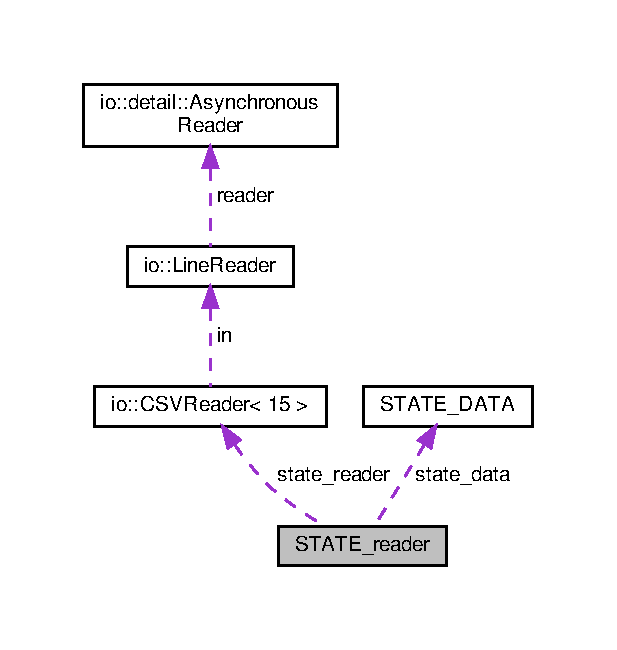
\includegraphics[width=296pt]{classSTATE__reader__coll__graph}
\end{center}
\end{figure}
\subsection*{Public Member Functions}
\begin{DoxyCompactItemize}
\item 
\mbox{\Hypertarget{classSTATE__reader_a5ad5acce808ca1ed4279ac7da1d5db4c}\label{classSTATE__reader_a5ad5acce808ca1ed4279ac7da1d5db4c}} 
{\bfseries S\+T\+A\+T\+E\+\_\+reader} (std\+::string filename)
\item 
\mbox{\Hypertarget{classSTATE__reader_a3af8f3f84ab16bb80089c19f14a40669}\label{classSTATE__reader_a3af8f3f84ab16bb80089c19f14a40669}} 
bool {\bfseries next\+Line} ()
\end{DoxyCompactItemize}
\subsection*{Public Attributes}
\begin{DoxyCompactItemize}
\item 
\mbox{\Hypertarget{classSTATE__reader_a4edbaa8ea1d2c7fb2fef27797dc45a50}\label{classSTATE__reader_a4edbaa8ea1d2c7fb2fef27797dc45a50}} 
\hyperlink{structSTATE__DATA}{S\+T\+A\+T\+E\+\_\+\+D\+A\+TA} {\bfseries state\+\_\+data}
\item 
\mbox{\Hypertarget{classSTATE__reader_a8d0e7b4ac753fa3e0bbbb891de83abfe}\label{classSTATE__reader_a8d0e7b4ac753fa3e0bbbb891de83abfe}} 
ros\+\_\+float\+::altitude\+State {\bfseries altitude\+From\+State\+Msg}
\item 
\mbox{\Hypertarget{classSTATE__reader_a9077b1dbc8ceb7363812334d3da43d29}\label{classSTATE__reader_a9077b1dbc8ceb7363812334d3da43d29}} 
ros\+\_\+float\+::ctl\+\_\+force {\bfseries ctl\+Force\+Msg}
\item 
\mbox{\Hypertarget{classSTATE__reader_a42ac50d81050a09f1f932e04b321e3bc}\label{classSTATE__reader_a42ac50d81050a09f1f932e04b321e3bc}} 
ros\+\_\+float\+::ctl\+\_\+force\+\_\+high {\bfseries ctl\+Force\+Hight\+Msg}
\item 
\mbox{\Hypertarget{classSTATE__reader_ad5600aac8ba36aa41cb6bfa0a91621ab}\label{classSTATE__reader_ad5600aac8ba36aa41cb6bfa0a91621ab}} 
ros\+\_\+float\+::ctl\+\_\+force\+\_\+low {\bfseries ctl\+Force\+Low\+Msg}
\item 
\mbox{\Hypertarget{classSTATE__reader_a83b57bc0d2ffa8d166cddceeb45bb820}\label{classSTATE__reader_a83b57bc0d2ffa8d166cddceeb45bb820}} 
ros\+\_\+float\+::ctl\+\_\+mode {\bfseries ctl\+Mode\+Msg}
\item 
\mbox{\Hypertarget{classSTATE__reader_a6176f057dced1febe1d199f965632c27}\label{classSTATE__reader_a6176f057dced1febe1d199f965632c27}} 
ros\+\_\+float\+::ctl\+\_\+status {\bfseries ctl\+Status\+Msg}
\item 
\mbox{\Hypertarget{classSTATE__reader_af54392524bbc9d255f56245a01ba1d17}\label{classSTATE__reader_af54392524bbc9d255f56245a01ba1d17}} 
ros\+\_\+float\+::depth\+From\+State {\bfseries depth\+From\+State\+Msg}
\item 
\mbox{\Hypertarget{classSTATE__reader_af245fa22b9eddb4980ffc95651ea4800}\label{classSTATE__reader_af245fa22b9eddb4980ffc95651ea4800}} 
ros\+\_\+float\+::in\+\_\+water {\bfseries in\+Water\+Msg}
\item 
\mbox{\Hypertarget{classSTATE__reader_a93364eba6232b52e190f40dfa24dc7ce}\label{classSTATE__reader_a93364eba6232b52e190f40dfa24dc7ce}} 
ros\+\_\+float\+::thrust\+\_\+cmd {\bfseries thrust\+Cmd\+Msg}
\item 
\mbox{\Hypertarget{classSTATE__reader_a6410f8402db53ac32f8f9acc0497c688}\label{classSTATE__reader_a6410f8402db53ac32f8f9acc0497c688}} 
ros\+\_\+float\+::traj\+\_\+vel {\bfseries traj\+Vel\+Msg}
\item 
\mbox{\Hypertarget{classSTATE__reader_acd1b627deab82b59ac115e7145a2deae}\label{classSTATE__reader_acd1b627deab82b59ac115e7145a2deae}} 
ros\+\_\+float\+::volume\+\_\+cmd {\bfseries volume\+Cmd\+Msg}
\item 
\mbox{\Hypertarget{classSTATE__reader_ae5dc8cfe4eade7a8678ef6cc88a4631a}\label{classSTATE__reader_ae5dc8cfe4eade7a8678ef6cc88a4631a}} 
ros\+\_\+float\+::volume\+Mode\+\_\+cmd {\bfseries volume\+Mode\+Msg}
\item 
\mbox{\Hypertarget{classSTATE__reader_a4b94f921036ff4fbe401065a75946655}\label{classSTATE__reader_a4b94f921036ff4fbe401065a75946655}} 
ros\+\_\+float\+::volume\+Rate\+\_\+cmd {\bfseries volume\+Rate\+Msg}
\item 
\mbox{\Hypertarget{classSTATE__reader_aafd4bfba38382d9234a5f555b9225912}\label{classSTATE__reader_aafd4bfba38382d9234a5f555b9225912}} 
ros\+\_\+float\+::zvelocity {\bfseries z\+Velocity\+Msg}
\end{DoxyCompactItemize}
\subsection*{Private Member Functions}
\begin{DoxyCompactItemize}
\item 
\mbox{\Hypertarget{classSTATE__reader_ac6039aa79525ccf563dff9533ad73e61}\label{classSTATE__reader_ac6039aa79525ccf563dff9533ad73e61}} 
void {\bfseries pack\+\_\+\+State\+\_\+\+Altitude\+\_\+\+Msg} ()
\item 
\mbox{\Hypertarget{classSTATE__reader_a26bf79b10d1a03997a1d67d2042597cd}\label{classSTATE__reader_a26bf79b10d1a03997a1d67d2042597cd}} 
void {\bfseries pack\+\_\+\+Ctl\+\_\+\+Force\+Msg} ()
\item 
\mbox{\Hypertarget{classSTATE__reader_af49b7d23c8485ecf1b2bb4bc5750a92c}\label{classSTATE__reader_af49b7d23c8485ecf1b2bb4bc5750a92c}} 
void {\bfseries pack\+\_\+\+Ctl\+\_\+\+Force\+\_\+\+High\+\_\+\+Msg} ()
\item 
\mbox{\Hypertarget{classSTATE__reader_aebe95f57ffbe91c5e476332fdabd875d}\label{classSTATE__reader_aebe95f57ffbe91c5e476332fdabd875d}} 
void {\bfseries pack\+\_\+\+Ctl\+\_\+\+Force\+\_\+\+Low\+\_\+\+Msg} ()
\item 
\mbox{\Hypertarget{classSTATE__reader_a408df34fba0495e11815a5496e788bf2}\label{classSTATE__reader_a408df34fba0495e11815a5496e788bf2}} 
void {\bfseries pack\+\_\+\+Ctl\+\_\+\+Mode\+\_\+\+Msg} ()
\item 
\mbox{\Hypertarget{classSTATE__reader_adc74eeeaf4ae6dfe09969a5969f23da2}\label{classSTATE__reader_adc74eeeaf4ae6dfe09969a5969f23da2}} 
void {\bfseries pack\+\_\+\+Ctl\+\_\+\+Status\+\_\+\+Msg} ()
\item 
\mbox{\Hypertarget{classSTATE__reader_a9dd459012dfb01e0df4139e67552f7b3}\label{classSTATE__reader_a9dd459012dfb01e0df4139e67552f7b3}} 
void {\bfseries pack\+\_\+\+Depth\+\_\+\+Msg} ()
\item 
\mbox{\Hypertarget{classSTATE__reader_a04869d6faec3302dd90e4b2b57b84142}\label{classSTATE__reader_a04869d6faec3302dd90e4b2b57b84142}} 
void {\bfseries pack\+\_\+\+In\+\_\+\+Water\+\_\+\+Msg} ()
\item 
\mbox{\Hypertarget{classSTATE__reader_ad834d9a70b1d7cc2ed0e96d0e50e94a9}\label{classSTATE__reader_ad834d9a70b1d7cc2ed0e96d0e50e94a9}} 
void {\bfseries pack\+\_\+\+Thrust\+\_\+\+Cmd\+\_\+\+Msg} ()
\item 
\mbox{\Hypertarget{classSTATE__reader_ac873b20c9bb3ade796f58d2c2bdfab59}\label{classSTATE__reader_ac873b20c9bb3ade796f58d2c2bdfab59}} 
void {\bfseries pack\+\_\+\+Traj\+\_\+\+Vel\+\_\+\+Msg} ()
\item 
\mbox{\Hypertarget{classSTATE__reader_a3d666eec14997c9fe74978abdc5a0fba}\label{classSTATE__reader_a3d666eec14997c9fe74978abdc5a0fba}} 
void {\bfseries pack\+\_\+\+Volume\+\_\+\+Cmd\+\_\+\+Msg} ()
\item 
\mbox{\Hypertarget{classSTATE__reader_a28ec1eb37c188f7ee1b6ebaf80d51139}\label{classSTATE__reader_a28ec1eb37c188f7ee1b6ebaf80d51139}} 
void {\bfseries pack\+\_\+\+Volume\+\_\+\+Mode\+\_\+\+Msg} ()
\item 
\mbox{\Hypertarget{classSTATE__reader_a5d4dd5f96e71324ce7ff8f6eadb24013}\label{classSTATE__reader_a5d4dd5f96e71324ce7ff8f6eadb24013}} 
void {\bfseries pack\+\_\+\+Volume\+\_\+\+Rate\+\_\+\+Msg} ()
\item 
\mbox{\Hypertarget{classSTATE__reader_a64549c42833730c3dbf13034be5303af}\label{classSTATE__reader_a64549c42833730c3dbf13034be5303af}} 
void {\bfseries pack\+\_\+\+Z\+Velocity\+\_\+\+Msg} ()
\end{DoxyCompactItemize}
\subsection*{Private Attributes}
\begin{DoxyCompactItemize}
\item 
\mbox{\Hypertarget{classSTATE__reader_a7b5c2cf312aeeffb3f0d46f9c25f79a4}\label{classSTATE__reader_a7b5c2cf312aeeffb3f0d46f9c25f79a4}} 
\hyperlink{classio_1_1CSVReader}{io\+::\+C\+S\+V\+Reader}$<$ 15 $>$ {\bfseries state\+\_\+reader}
\item 
\mbox{\Hypertarget{classSTATE__reader_a03c62544f89afb1f3b05d87676b574c8}\label{classSTATE__reader_a03c62544f89afb1f3b05d87676b574c8}} 
unsigned int {\bfseries msg\+Num\+State}
\end{DoxyCompactItemize}


The documentation for this class was generated from the following files\+:\begin{DoxyCompactItemize}
\item 
/home/emanuele/catkin\+\_\+ws/src/ros\+\_\+float/include/ros\+\_\+float/state\+\_\+reader.\+h\item 
/home/emanuele/catkin\+\_\+ws/src/ros\+\_\+float/include/ros\+\_\+float/state\+\_\+reader.\+cpp\end{DoxyCompactItemize}

\hypertarget{classio_1_1detail_1_1SynchronousReader}{}\section{io\+:\+:detail\+:\+:Synchronous\+Reader Class Reference}
\label{classio_1_1detail_1_1SynchronousReader}\index{io\+::detail\+::\+Synchronous\+Reader@{io\+::detail\+::\+Synchronous\+Reader}}
\subsection*{Public Member Functions}
\begin{DoxyCompactItemize}
\item 
\mbox{\Hypertarget{classio_1_1detail_1_1SynchronousReader_a4dc78563ff667b92ad3096a94e834eb5}\label{classio_1_1detail_1_1SynchronousReader_a4dc78563ff667b92ad3096a94e834eb5}} 
void {\bfseries init} (std\+::unique\+\_\+ptr$<$ \hyperlink{classio_1_1ByteSourceBase}{Byte\+Source\+Base} $>$arg\+\_\+byte\+\_\+source)
\item 
\mbox{\Hypertarget{classio_1_1detail_1_1SynchronousReader_a9d6b2c888cc7020df1bb81c8bb5c58bc}\label{classio_1_1detail_1_1SynchronousReader_a9d6b2c888cc7020df1bb81c8bb5c58bc}} 
bool {\bfseries is\+\_\+valid} () const
\item 
\mbox{\Hypertarget{classio_1_1detail_1_1SynchronousReader_a6cad1371b97e14f660914898b16433c4}\label{classio_1_1detail_1_1SynchronousReader_a6cad1371b97e14f660914898b16433c4}} 
void {\bfseries start\+\_\+read} (char $\ast$arg\+\_\+buffer, int arg\+\_\+desired\+\_\+byte\+\_\+count)
\item 
\mbox{\Hypertarget{classio_1_1detail_1_1SynchronousReader_a519a0cb25c641d2e51b6542749c44606}\label{classio_1_1detail_1_1SynchronousReader_a519a0cb25c641d2e51b6542749c44606}} 
int {\bfseries finish\+\_\+read} ()
\end{DoxyCompactItemize}
\subsection*{Private Attributes}
\begin{DoxyCompactItemize}
\item 
\mbox{\Hypertarget{classio_1_1detail_1_1SynchronousReader_aa4ab4d5029b7d438051b4c800292059d}\label{classio_1_1detail_1_1SynchronousReader_aa4ab4d5029b7d438051b4c800292059d}} 
std\+::unique\+\_\+ptr$<$ \hyperlink{classio_1_1ByteSourceBase}{Byte\+Source\+Base} $>$ {\bfseries byte\+\_\+source}
\item 
\mbox{\Hypertarget{classio_1_1detail_1_1SynchronousReader_aa57e237e05bd90abdd9e896647da3fc7}\label{classio_1_1detail_1_1SynchronousReader_aa57e237e05bd90abdd9e896647da3fc7}} 
char $\ast$ {\bfseries buffer}
\item 
\mbox{\Hypertarget{classio_1_1detail_1_1SynchronousReader_ac85e7a1b24cd383fb9fbfafe648f9ad6}\label{classio_1_1detail_1_1SynchronousReader_ac85e7a1b24cd383fb9fbfafe648f9ad6}} 
int {\bfseries desired\+\_\+byte\+\_\+count}
\end{DoxyCompactItemize}


The documentation for this class was generated from the following file\+:\begin{DoxyCompactItemize}
\item 
/home/emanuele/catkin\+\_\+ws/src/ros\+\_\+float/include/ros\+\_\+float/csv.\+h\end{DoxyCompactItemize}

\hypertarget{structio_1_1throw__on__overflow}{}\section{io\+:\+:throw\+\_\+on\+\_\+overflow Struct Reference}
\label{structio_1_1throw__on__overflow}\index{io\+::throw\+\_\+on\+\_\+overflow@{io\+::throw\+\_\+on\+\_\+overflow}}
\subsection*{Static Public Member Functions}
\begin{DoxyCompactItemize}
\item 
\mbox{\Hypertarget{structio_1_1throw__on__overflow_a0a59c1dc2ead1a9275c62885ec7545d2}\label{structio_1_1throw__on__overflow_a0a59c1dc2ead1a9275c62885ec7545d2}} 
{\footnotesize template$<$class T $>$ }\\static void {\bfseries on\+\_\+overflow} (T \&)
\item 
\mbox{\Hypertarget{structio_1_1throw__on__overflow_a2ae91b1ae3d655c16f7e6a7e9a1abd92}\label{structio_1_1throw__on__overflow_a2ae91b1ae3d655c16f7e6a7e9a1abd92}} 
{\footnotesize template$<$class T $>$ }\\static void {\bfseries on\+\_\+underflow} (T \&)
\end{DoxyCompactItemize}


The documentation for this struct was generated from the following file\+:\begin{DoxyCompactItemize}
\item 
/home/emanuele/catkin\+\_\+ws/src/ros\+\_\+float/include/ros\+\_\+float/csv.\+h\end{DoxyCompactItemize}

\hypertarget{structio_1_1error_1_1too__few__columns}{}\section{io\+:\+:error\+:\+:too\+\_\+few\+\_\+columns Struct Reference}
\label{structio_1_1error_1_1too__few__columns}\index{io\+::error\+::too\+\_\+few\+\_\+columns@{io\+::error\+::too\+\_\+few\+\_\+columns}}


Inheritance diagram for io\+:\+:error\+:\+:too\+\_\+few\+\_\+columns\+:\nopagebreak
\begin{figure}[H]
\begin{center}
\leavevmode
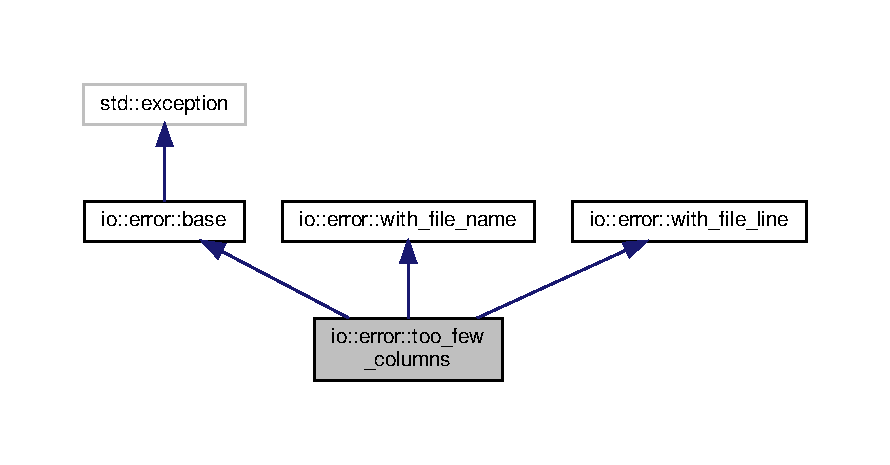
\includegraphics[width=350pt]{structio_1_1error_1_1too__few__columns__inherit__graph}
\end{center}
\end{figure}


Collaboration diagram for io\+:\+:error\+:\+:too\+\_\+few\+\_\+columns\+:\nopagebreak
\begin{figure}[H]
\begin{center}
\leavevmode
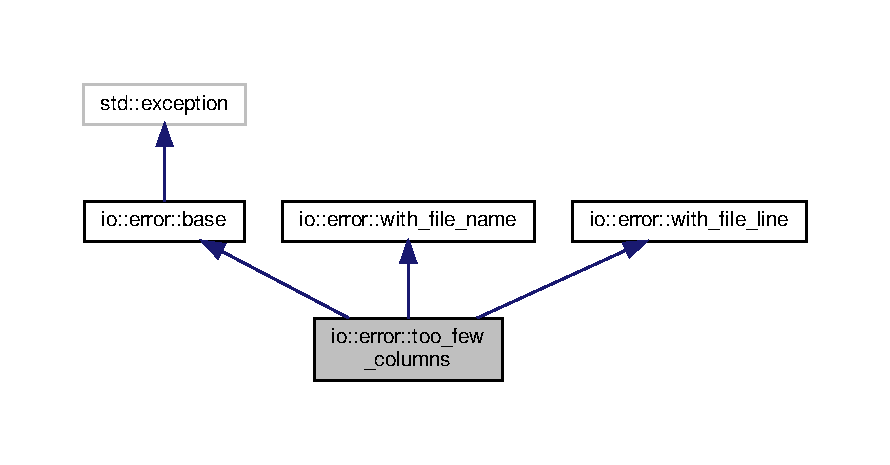
\includegraphics[width=350pt]{structio_1_1error_1_1too__few__columns__coll__graph}
\end{center}
\end{figure}
\subsection*{Public Member Functions}
\begin{DoxyCompactItemize}
\item 
\mbox{\Hypertarget{structio_1_1error_1_1too__few__columns_a58d6d1fada127120facbcc00851ab455}\label{structio_1_1error_1_1too__few__columns_a58d6d1fada127120facbcc00851ab455}} 
void {\bfseries format\+\_\+error\+\_\+message} () const
\end{DoxyCompactItemize}
\subsection*{Additional Inherited Members}


The documentation for this struct was generated from the following file\+:\begin{DoxyCompactItemize}
\item 
/home/emanuele/catkin\+\_\+ws/src/ros\+\_\+float/include/ros\+\_\+float/csv.\+h\end{DoxyCompactItemize}

\hypertarget{structio_1_1error_1_1too__many__columns}{}\section{io\+:\+:error\+:\+:too\+\_\+many\+\_\+columns Struct Reference}
\label{structio_1_1error_1_1too__many__columns}\index{io\+::error\+::too\+\_\+many\+\_\+columns@{io\+::error\+::too\+\_\+many\+\_\+columns}}


Inheritance diagram for io\+:\+:error\+:\+:too\+\_\+many\+\_\+columns\+:\nopagebreak
\begin{figure}[H]
\begin{center}
\leavevmode
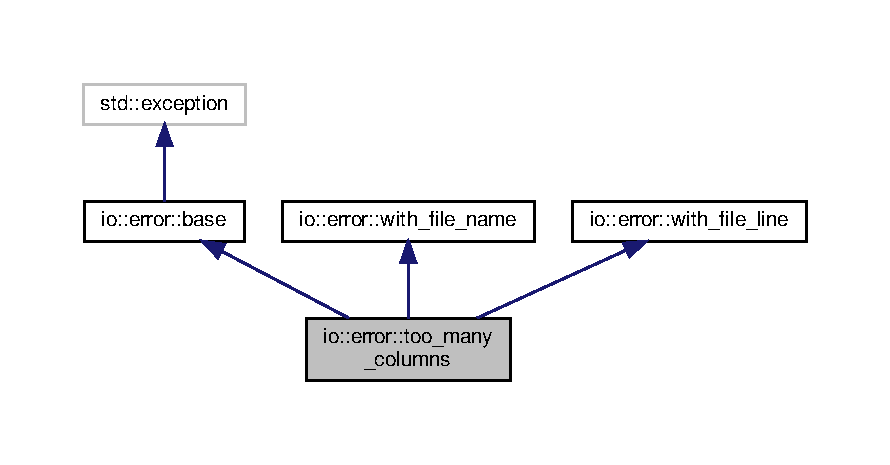
\includegraphics[width=350pt]{structio_1_1error_1_1too__many__columns__inherit__graph}
\end{center}
\end{figure}


Collaboration diagram for io\+:\+:error\+:\+:too\+\_\+many\+\_\+columns\+:\nopagebreak
\begin{figure}[H]
\begin{center}
\leavevmode
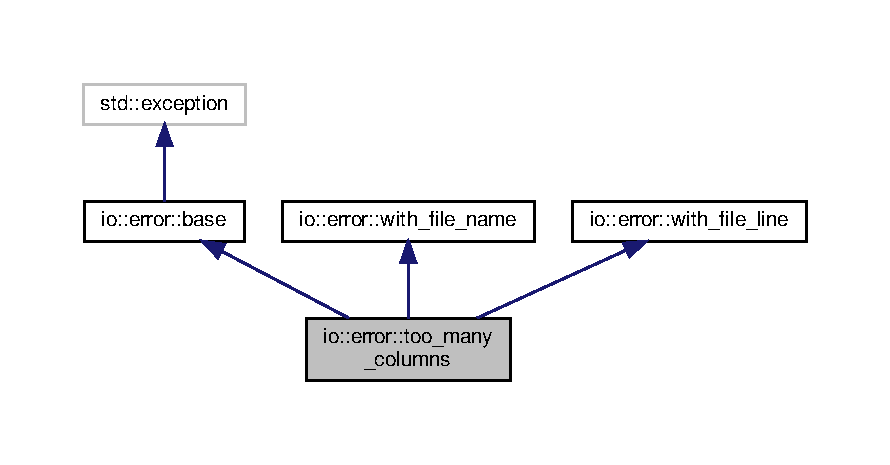
\includegraphics[width=350pt]{structio_1_1error_1_1too__many__columns__coll__graph}
\end{center}
\end{figure}
\subsection*{Public Member Functions}
\begin{DoxyCompactItemize}
\item 
\mbox{\Hypertarget{structio_1_1error_1_1too__many__columns_a2072af07b0408387579becc076a9809e}\label{structio_1_1error_1_1too__many__columns_a2072af07b0408387579becc076a9809e}} 
void {\bfseries format\+\_\+error\+\_\+message} () const
\end{DoxyCompactItemize}
\subsection*{Additional Inherited Members}


The documentation for this struct was generated from the following file\+:\begin{DoxyCompactItemize}
\item 
/home/emanuele/catkin\+\_\+ws/src/ros\+\_\+float/include/ros\+\_\+float/csv.\+h\end{DoxyCompactItemize}

\hypertarget{structio_1_1trim__chars}{}\section{io\+:\+:trim\+\_\+chars$<$ trim\+\_\+char\+\_\+list $>$ Struct Template Reference}
\label{structio_1_1trim__chars}\index{io\+::trim\+\_\+chars$<$ trim\+\_\+char\+\_\+list $>$@{io\+::trim\+\_\+chars$<$ trim\+\_\+char\+\_\+list $>$}}
\subsection*{Static Public Member Functions}
\begin{DoxyCompactItemize}
\item 
\mbox{\Hypertarget{structio_1_1trim__chars_a4cffc5e839ab4024ca8c8330e26e338c}\label{structio_1_1trim__chars_a4cffc5e839ab4024ca8c8330e26e338c}} 
static void {\bfseries trim} (char $\ast$\&str\+\_\+begin, char $\ast$\&str\+\_\+end)
\end{DoxyCompactItemize}
\subsection*{Static Private Member Functions}
\begin{DoxyCompactItemize}
\item 
\mbox{\Hypertarget{structio_1_1trim__chars_a8868df0aa3887f5968cab2fac9c746fb}\label{structio_1_1trim__chars_a8868df0aa3887f5968cab2fac9c746fb}} 
static constexpr bool {\bfseries is\+\_\+trim\+\_\+char} (char)
\item 
\mbox{\Hypertarget{structio_1_1trim__chars_a4c365acae57f96990d08e9b4c6a89e48}\label{structio_1_1trim__chars_a4c365acae57f96990d08e9b4c6a89e48}} 
{\footnotesize template$<$class ... Other\+Trim\+Chars$>$ }\\static constexpr bool {\bfseries is\+\_\+trim\+\_\+char} (char c, char trim\+\_\+char, Other\+Trim\+Chars...\+other\+\_\+trim\+\_\+chars)
\end{DoxyCompactItemize}


The documentation for this struct was generated from the following file\+:\begin{DoxyCompactItemize}
\item 
/home/emanuele/catkin\+\_\+ws/src/ros\+\_\+float/include/ros\+\_\+float/csv.\+h\end{DoxyCompactItemize}

\hypertarget{structUM6__DATA}{}\section{U\+M6\+\_\+\+D\+A\+TA Struct Reference}
\label{structUM6__DATA}\index{U\+M6\+\_\+\+D\+A\+TA@{U\+M6\+\_\+\+D\+A\+TA}}
\subsection*{Public Attributes}
\begin{DoxyCompactItemize}
\item 
\mbox{\Hypertarget{structUM6__DATA_ab432152c206ac734189c3376793e296f}\label{structUM6__DATA_ab432152c206ac734189c3376793e296f}} 
double {\bfseries magz}
\item 
\mbox{\Hypertarget{structUM6__DATA_a3d3764f71a27a910cc2efedc1efefe9e}\label{structUM6__DATA_a3d3764f71a27a910cc2efedc1efefe9e}} 
double {\bfseries magy}
\item 
\mbox{\Hypertarget{structUM6__DATA_a7c5fb0dae9e66418cac743cabdfeba8a}\label{structUM6__DATA_a7c5fb0dae9e66418cac743cabdfeba8a}} 
double {\bfseries magx}
\item 
\mbox{\Hypertarget{structUM6__DATA_a0a1efe884e8f84d5f17bf2f01f706e83}\label{structUM6__DATA_a0a1efe884e8f84d5f17bf2f01f706e83}} 
float {\bfseries accelz}
\item 
\mbox{\Hypertarget{structUM6__DATA_a1bb8ccce29ea98667dd067d5f1fb2d18}\label{structUM6__DATA_a1bb8ccce29ea98667dd067d5f1fb2d18}} 
float {\bfseries accelx}
\item 
\mbox{\Hypertarget{structUM6__DATA_a10f5233fec4023a090abc979f1c45142}\label{structUM6__DATA_a10f5233fec4023a090abc979f1c45142}} 
float {\bfseries accely}
\item 
\mbox{\Hypertarget{structUM6__DATA_aca698bcfa633ec72f856ec2be0529451}\label{structUM6__DATA_aca698bcfa633ec72f856ec2be0529451}} 
unsigned long {\bfseries timestamp}
\item 
\mbox{\Hypertarget{structUM6__DATA_a109dcf93fe90bb75f976a886fb1a804d}\label{structUM6__DATA_a109dcf93fe90bb75f976a886fb1a804d}} 
double \hyperlink{structUM6__DATA_a109dcf93fe90bb75f976a886fb1a804d}{phi}
\begin{DoxyCompactList}\small\item\em F\+I\+X\+ME uint64\+\_\+t? \end{DoxyCompactList}\item 
\mbox{\Hypertarget{structUM6__DATA_a4939eb18ae1915ccf6d3173342c5bdba}\label{structUM6__DATA_a4939eb18ae1915ccf6d3173342c5bdba}} 
double {\bfseries psi}
\item 
\mbox{\Hypertarget{structUM6__DATA_a2c177fae05469423024e3959b2b8d3f5}\label{structUM6__DATA_a2c177fae05469423024e3959b2b8d3f5}} 
double {\bfseries theta}
\item 
\mbox{\Hypertarget{structUM6__DATA_a789182c4d5cd5ef5e354d3c6948b91e3}\label{structUM6__DATA_a789182c4d5cd5ef5e354d3c6948b91e3}} 
double {\bfseries gyrox}
\item 
\mbox{\Hypertarget{structUM6__DATA_a54092125813f72dc4fdf4c14a7a6ce36}\label{structUM6__DATA_a54092125813f72dc4fdf4c14a7a6ce36}} 
double {\bfseries gyroy}
\item 
\mbox{\Hypertarget{structUM6__DATA_a66cbd5d8aa21a4c746374a8afac9e5f1}\label{structUM6__DATA_a66cbd5d8aa21a4c746374a8afac9e5f1}} 
double {\bfseries gyroz}
\end{DoxyCompactItemize}


The documentation for this struct was generated from the following file\+:\begin{DoxyCompactItemize}
\item 
/home/emanuele/catkin\+\_\+ws/src/ros\+\_\+float/include/ros\+\_\+float/um6\+\_\+reader.\+h\end{DoxyCompactItemize}

\hypertarget{classUM6__reader}{}\section{U\+M6\+\_\+reader Class Reference}
\label{classUM6__reader}\index{U\+M6\+\_\+reader@{U\+M6\+\_\+reader}}


Collaboration diagram for U\+M6\+\_\+reader\+:\nopagebreak
\begin{figure}[H]
\begin{center}
\leavevmode
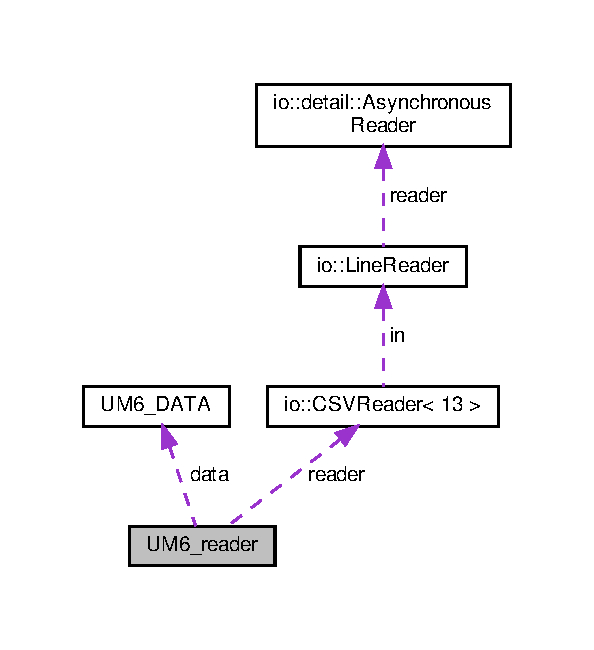
\includegraphics[width=285pt]{classUM6__reader__coll__graph}
\end{center}
\end{figure}
\subsection*{Public Member Functions}
\begin{DoxyCompactItemize}
\item 
\mbox{\Hypertarget{classUM6__reader_a4c1e7e60a4ad6c5387456df9f5642880}\label{classUM6__reader_a4c1e7e60a4ad6c5387456df9f5642880}} 
{\bfseries U\+M6\+\_\+reader} (std\+::string filename)
\item 
\mbox{\Hypertarget{classUM6__reader_a1886d8398f9590ed762a92603663272f}\label{classUM6__reader_a1886d8398f9590ed762a92603663272f}} 
bool {\bfseries next\+Line} ()
\end{DoxyCompactItemize}
\subsection*{Public Attributes}
\begin{DoxyCompactItemize}
\item 
\mbox{\Hypertarget{classUM6__reader_a7f50e5345f41317f98483698f94b8a0a}\label{classUM6__reader_a7f50e5345f41317f98483698f94b8a0a}} 
\hyperlink{structUM6__DATA}{U\+M6\+\_\+\+D\+A\+TA} {\bfseries data}
\item 
\mbox{\Hypertarget{classUM6__reader_a8125a580ce28b4832482eadee969914c}\label{classUM6__reader_a8125a580ce28b4832482eadee969914c}} 
sensor\+\_\+msgs\+::\+Imu {\bfseries imu\+Msg}
\item 
\mbox{\Hypertarget{classUM6__reader_adf090821e5feb18b0c1a7b360b459117}\label{classUM6__reader_adf090821e5feb18b0c1a7b360b459117}} 
sensor\+\_\+msgs\+::\+Magnetic\+Field {\bfseries mag\+Msg}
\end{DoxyCompactItemize}
\subsection*{Private Member Functions}
\begin{DoxyCompactItemize}
\item 
\mbox{\Hypertarget{classUM6__reader_a180ef21f2b44ba6424b085683733d499}\label{classUM6__reader_a180ef21f2b44ba6424b085683733d499}} 
void {\bfseries pack\+Imu\+Msg} ()
\item 
\mbox{\Hypertarget{classUM6__reader_a97a73a034843017ed137be83d4c9b80f}\label{classUM6__reader_a97a73a034843017ed137be83d4c9b80f}} 
void {\bfseries pack\+Mag\+Msg} ()
\end{DoxyCompactItemize}
\subsection*{Private Attributes}
\begin{DoxyCompactItemize}
\item 
\mbox{\Hypertarget{classUM6__reader_adb7e15fec787175b180bad466a428b09}\label{classUM6__reader_adb7e15fec787175b180bad466a428b09}} 
\hyperlink{classio_1_1CSVReader}{io\+::\+C\+S\+V\+Reader}$<$ 13 $>$ {\bfseries reader}
\item 
\mbox{\Hypertarget{classUM6__reader_a64f023ad297d475d79a17a2e8ac17d93}\label{classUM6__reader_a64f023ad297d475d79a17a2e8ac17d93}} 
unsigned int {\bfseries msg\+Num}
\end{DoxyCompactItemize}


The documentation for this class was generated from the following files\+:\begin{DoxyCompactItemize}
\item 
/home/emanuele/catkin\+\_\+ws/src/ros\+\_\+float/include/ros\+\_\+float/um6\+\_\+reader.\+h\item 
/home/emanuele/catkin\+\_\+ws/src/ros\+\_\+float/include/ros\+\_\+float/um6\+\_\+reader.\+cpp\end{DoxyCompactItemize}

\hypertarget{structUSBL__DATA}{}\section{U\+S\+B\+L\+\_\+\+D\+A\+TA Struct Reference}
\label{structUSBL__DATA}\index{U\+S\+B\+L\+\_\+\+D\+A\+TA@{U\+S\+B\+L\+\_\+\+D\+A\+TA}}
\subsection*{Public Attributes}
\begin{DoxyCompactItemize}
\item 
\mbox{\Hypertarget{structUSBL__DATA_a18673df92f4c80a326016b28798f6dfc}\label{structUSBL__DATA_a18673df92f4c80a326016b28798f6dfc}} 
int {\bfseries prop\+\_\+time}
\item 
\mbox{\Hypertarget{structUSBL__DATA_adb9cabe0a315feeb2f26dab5fa8d8c20}\label{structUSBL__DATA_adb9cabe0a315feeb2f26dab5fa8d8c20}} 
double {\bfseries accuracy}
\item 
\mbox{\Hypertarget{structUSBL__DATA_a151e339829d8d6b8caa82c88f983c44d}\label{structUSBL__DATA_a151e339829d8d6b8caa82c88f983c44d}} 
double {\bfseries e\+\_\+reader}
\item 
\mbox{\Hypertarget{structUSBL__DATA_adf15833806125118c347644d01aa08fd}\label{structUSBL__DATA_adf15833806125118c347644d01aa08fd}} 
unsigned long {\bfseries ctime}
\item 
\mbox{\Hypertarget{structUSBL__DATA_aaf5c26e66fb2c53eda8639cf9865708d}\label{structUSBL__DATA_aaf5c26e66fb2c53eda8639cf9865708d}} 
double {\bfseries h\+\_\+reader}
\item 
\mbox{\Hypertarget{structUSBL__DATA_ab54b630ba7565b0eb7008283ea064e1b}\label{structUSBL__DATA_ab54b630ba7565b0eb7008283ea064e1b}} 
int {\bfseries remote\+\_\+id}
\item 
\mbox{\Hypertarget{structUSBL__DATA_ab871395e915e4278906a3a2f4348fb94}\label{structUSBL__DATA_ab871395e915e4278906a3a2f4348fb94}} 
int {\bfseries rssi}
\item 
\mbox{\Hypertarget{structUSBL__DATA_abf1b91b10f868316677fe3170a11e2c1}\label{structUSBL__DATA_abf1b91b10f868316677fe3170a11e2c1}} 
double {\bfseries n\+\_\+reader}
\item 
\mbox{\Hypertarget{structUSBL__DATA_a7a6b598b2c48105a5361c0eb16113c5a}\label{structUSBL__DATA_a7a6b598b2c48105a5361c0eb16113c5a}} 
double {\bfseries p\+\_\+reader}
\item 
\mbox{\Hypertarget{structUSBL__DATA_a35000c42568d33ae46ec4e9923f2738d}\label{structUSBL__DATA_a35000c42568d33ae46ec4e9923f2738d}} 
double {\bfseries depth\+U\+S\+BL}
\item 
\mbox{\Hypertarget{structUSBL__DATA_a102106844aee9e04e45629573ef99dbf}\label{structUSBL__DATA_a102106844aee9e04e45629573ef99dbf}} 
double {\bfseries r\+\_\+reader}
\item 
\mbox{\Hypertarget{structUSBL__DATA_a58fa02be969674c1298117356525f0f2}\label{structUSBL__DATA_a58fa02be969674c1298117356525f0f2}} 
double {\bfseries u\+\_\+reader}
\item 
\mbox{\Hypertarget{structUSBL__DATA_aa3cd83c0023ee88d8630f1325281cfd2}\label{structUSBL__DATA_aa3cd83c0023ee88d8630f1325281cfd2}} 
unsigned long {\bfseries mtime}
\item 
\mbox{\Hypertarget{structUSBL__DATA_a26db296587adb3d461315d3ab347c8ad}\label{structUSBL__DATA_a26db296587adb3d461315d3ab347c8ad}} 
double {\bfseries x\+Position}
\item 
\mbox{\Hypertarget{structUSBL__DATA_a665becdbc39316141aa5a8dd4f41fc18}\label{structUSBL__DATA_a665becdbc39316141aa5a8dd4f41fc18}} 
double {\bfseries y\+Position}
\item 
\mbox{\Hypertarget{structUSBL__DATA_ab1770760f66b5d2ecbd34cfbfcb99c30}\label{structUSBL__DATA_ab1770760f66b5d2ecbd34cfbfcb99c30}} 
double {\bfseries z\+Position}
\item 
\mbox{\Hypertarget{structUSBL__DATA_a3accab090f58fa86babe87c310cae06b}\label{structUSBL__DATA_a3accab090f58fa86babe87c310cae06b}} 
int {\bfseries integrity}
\item 
\mbox{\Hypertarget{structUSBL__DATA_ab2ad8c42689b180c0677782c14868aa0}\label{structUSBL__DATA_ab2ad8c42689b180c0677782c14868aa0}} 
unsigned {\bfseries timestamp}
\end{DoxyCompactItemize}


The documentation for this struct was generated from the following file\+:\begin{DoxyCompactItemize}
\item 
/home/emanuele/catkin\+\_\+ws/src/ros\+\_\+float/include/ros\+\_\+float/usbl\+\_\+reader.\+h\end{DoxyCompactItemize}

\hypertarget{classUSBL__reader}{}\section{U\+S\+B\+L\+\_\+reader Class Reference}
\label{classUSBL__reader}\index{U\+S\+B\+L\+\_\+reader@{U\+S\+B\+L\+\_\+reader}}


Collaboration diagram for U\+S\+B\+L\+\_\+reader\+:\nopagebreak
\begin{figure}[H]
\begin{center}
\leavevmode
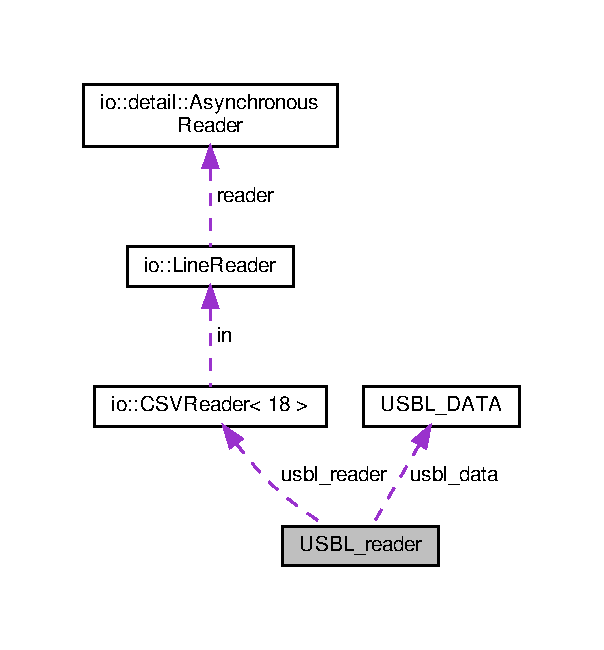
\includegraphics[width=290pt]{classUSBL__reader__coll__graph}
\end{center}
\end{figure}
\subsection*{Public Member Functions}
\begin{DoxyCompactItemize}
\item 
\mbox{\Hypertarget{classUSBL__reader_a80d29b2cda4006b7764d4fe8d855afcc}\label{classUSBL__reader_a80d29b2cda4006b7764d4fe8d855afcc}} 
{\bfseries U\+S\+B\+L\+\_\+reader} (std\+::string filename)
\item 
\mbox{\Hypertarget{classUSBL__reader_a7653a3792b19dc442ab5d8502422db2a}\label{classUSBL__reader_a7653a3792b19dc442ab5d8502422db2a}} 
bool {\bfseries next\+Line} ()
\end{DoxyCompactItemize}
\subsection*{Public Attributes}
\begin{DoxyCompactItemize}
\item 
\mbox{\Hypertarget{classUSBL__reader_a7f13d393ab0eb642e8bdf8d88240a770}\label{classUSBL__reader_a7f13d393ab0eb642e8bdf8d88240a770}} 
\hyperlink{structUSBL__DATA}{U\+S\+B\+L\+\_\+\+D\+A\+TA} {\bfseries usbl\+\_\+data}
\item 
\mbox{\Hypertarget{classUSBL__reader_ac21b0b74ab3eabdc47a1eae893c7ba5e}\label{classUSBL__reader_ac21b0b74ab3eabdc47a1eae893c7ba5e}} 
ros\+\_\+float\+::accuracy {\bfseries accuracy\+Msg}
\item 
\mbox{\Hypertarget{classUSBL__reader_a0d06c236642fbb0481de6ed127448182}\label{classUSBL__reader_a0d06c236642fbb0481de6ed127448182}} 
ros\+\_\+float\+::ctime {\bfseries ctime\+Msg}
\item 
\mbox{\Hypertarget{classUSBL__reader_ae80813254f989867a41f903782573a7d}\label{classUSBL__reader_ae80813254f989867a41f903782573a7d}} 
ros\+\_\+float\+::e {\bfseries e\+Msg}
\item 
\mbox{\Hypertarget{classUSBL__reader_a5817411089ad2ba18fa9e848a823bbc9}\label{classUSBL__reader_a5817411089ad2ba18fa9e848a823bbc9}} 
ros\+\_\+float\+::h {\bfseries h\+Msg}
\item 
\mbox{\Hypertarget{classUSBL__reader_a6c48c3021f4aa2d702193f299872722f}\label{classUSBL__reader_a6c48c3021f4aa2d702193f299872722f}} 
ros\+\_\+float\+::integrity {\bfseries integraity\+Msg}
\item 
\mbox{\Hypertarget{classUSBL__reader_a4c07f2e6941a1917b23fa7d823c44890}\label{classUSBL__reader_a4c07f2e6941a1917b23fa7d823c44890}} 
ros\+\_\+float\+::mtime {\bfseries m\+Time\+Msg}
\item 
\mbox{\Hypertarget{classUSBL__reader_a528f42d692c29aef29fa4926098a9051}\label{classUSBL__reader_a528f42d692c29aef29fa4926098a9051}} 
ros\+\_\+float\+::n {\bfseries n\+Msg}
\item 
\mbox{\Hypertarget{classUSBL__reader_aa4442b7be4854be8d7b1824e2178f996}\label{classUSBL__reader_aa4442b7be4854be8d7b1824e2178f996}} 
ros\+\_\+float\+::p {\bfseries p\+Msg}
\item 
\mbox{\Hypertarget{classUSBL__reader_a8ee6fe97696c8817266f4931043d6eb3}\label{classUSBL__reader_a8ee6fe97696c8817266f4931043d6eb3}} 
ros\+\_\+float\+::prop\+\_\+time {\bfseries prop\+Timesg}
\item 
\mbox{\Hypertarget{classUSBL__reader_af8f9a03e453ff6a2e890854a1ac7b40f}\label{classUSBL__reader_af8f9a03e453ff6a2e890854a1ac7b40f}} 
ros\+\_\+float\+::r {\bfseries r\+Msg}
\item 
\mbox{\Hypertarget{classUSBL__reader_a3a9b97cb18160e7aa01631f7f48055d1}\label{classUSBL__reader_a3a9b97cb18160e7aa01631f7f48055d1}} 
ros\+\_\+float\+::remote\+\_\+id {\bfseries remote\+I\+D\+Msg}
\item 
\mbox{\Hypertarget{classUSBL__reader_ad0dce9112f8e2dcb78255e4a584e321d}\label{classUSBL__reader_ad0dce9112f8e2dcb78255e4a584e321d}} 
ros\+\_\+float\+::rssi {\bfseries rssi\+Msg}
\item 
\mbox{\Hypertarget{classUSBL__reader_a75c4c86c9ea8e8b73c2405d3928669f7}\label{classUSBL__reader_a75c4c86c9ea8e8b73c2405d3928669f7}} 
ros\+\_\+float\+::u {\bfseries u\+Msg}
\item 
\mbox{\Hypertarget{classUSBL__reader_a27d7c30d8986dfafe241068da2667807}\label{classUSBL__reader_a27d7c30d8986dfafe241068da2667807}} 
geometry\+\_\+msgs\+::\+Pose {\bfseries pose\+X\+Y\+Z\+Msg}
\item 
\mbox{\Hypertarget{classUSBL__reader_ac26c28b787458221bee245defb541788}\label{classUSBL__reader_ac26c28b787458221bee245defb541788}} 
geometry\+\_\+msgs\+::\+Pose\+With\+Covariance\+Stamped {\bfseries pose\+With\+Cov\+Stamped}
\end{DoxyCompactItemize}
\subsection*{Private Member Functions}
\begin{DoxyCompactItemize}
\item 
\mbox{\Hypertarget{classUSBL__reader_afa8b1d7df1e92dca0aab40dbe75ce52d}\label{classUSBL__reader_afa8b1d7df1e92dca0aab40dbe75ce52d}} 
void {\bfseries pack\+\_\+\+X\+Y\+Z\+\_\+\+Pose\+\_\+\+With\+Covariance\+\_\+\+Msg} ()
\item 
\mbox{\Hypertarget{classUSBL__reader_add8999e41a9e7f5b0e4e2a4b7ae8f272}\label{classUSBL__reader_add8999e41a9e7f5b0e4e2a4b7ae8f272}} 
void {\bfseries pack\+\_\+\+Prop\+\_\+\+Time\+\_\+\+Msg} ()
\item 
\mbox{\Hypertarget{classUSBL__reader_a11c38ebe64e4e4370dfb21c1b83ec35c}\label{classUSBL__reader_a11c38ebe64e4e4370dfb21c1b83ec35c}} 
void {\bfseries pack\+\_\+\+Accuracy\+\_\+\+Msg} ()
\item 
\mbox{\Hypertarget{classUSBL__reader_a9f6a69fc0441c9ed2c3f4b622af2fa23}\label{classUSBL__reader_a9f6a69fc0441c9ed2c3f4b622af2fa23}} 
void {\bfseries pack\+\_\+\+E\+\_\+\+Msg} ()
\item 
\mbox{\Hypertarget{classUSBL__reader_ad70c647e424b4d1b1757794176ebabbd}\label{classUSBL__reader_ad70c647e424b4d1b1757794176ebabbd}} 
void {\bfseries pack\+\_\+\+C\+Time\+\_\+\+Msg} ()
\item 
\mbox{\Hypertarget{classUSBL__reader_a29ee3574cc5e3b1db3a2a4d2147111ce}\label{classUSBL__reader_a29ee3574cc5e3b1db3a2a4d2147111ce}} 
void {\bfseries pack\+\_\+\+H\+\_\+\+Msg} ()
\item 
\mbox{\Hypertarget{classUSBL__reader_a8f9edcefc5187ca5e9df99b9c769fb8d}\label{classUSBL__reader_a8f9edcefc5187ca5e9df99b9c769fb8d}} 
void {\bfseries pack\+\_\+remote\+\_\+\+I\+D\+\_\+\+Msg} ()
\item 
\mbox{\Hypertarget{classUSBL__reader_aa15748d7dca00be71d7526b698fdcdab}\label{classUSBL__reader_aa15748d7dca00be71d7526b698fdcdab}} 
void {\bfseries pack\+\_\+\+Rssi\+\_\+\+Msg} ()
\item 
\mbox{\Hypertarget{classUSBL__reader_a501267ad0000764024d02b7dc3d5da2f}\label{classUSBL__reader_a501267ad0000764024d02b7dc3d5da2f}} 
void {\bfseries pack\+\_\+\+N\+\_\+\+Msg} ()
\item 
\mbox{\Hypertarget{classUSBL__reader_a12bad474ef1abae5f851f6ca3081725b}\label{classUSBL__reader_a12bad474ef1abae5f851f6ca3081725b}} 
void {\bfseries pack\+\_\+\+P\+\_\+\+Msg} ()
\item 
\mbox{\Hypertarget{classUSBL__reader_a072218abbd50b9aa9134461a0f4ba9db}\label{classUSBL__reader_a072218abbd50b9aa9134461a0f4ba9db}} 
void {\bfseries pack\+\_\+\+R\+\_\+\+Msg} ()
\item 
\mbox{\Hypertarget{classUSBL__reader_abcfef373d8b093536d49690834f3a7de}\label{classUSBL__reader_abcfef373d8b093536d49690834f3a7de}} 
void {\bfseries pack\+\_\+\+U\+\_\+\+Msg} ()
\item 
\mbox{\Hypertarget{classUSBL__reader_a2f618419b912f70c2096913d0b62240f}\label{classUSBL__reader_a2f618419b912f70c2096913d0b62240f}} 
void {\bfseries pack\+\_\+\+M\+Time\+\_\+\+Msg} ()
\item 
\mbox{\Hypertarget{classUSBL__reader_a330c1291d48f63a51783d2ae267a978c}\label{classUSBL__reader_a330c1291d48f63a51783d2ae267a978c}} 
void {\bfseries pack\+\_\+\+Integrity\+\_\+\+Msg} ()
\item 
\mbox{\Hypertarget{classUSBL__reader_af0185260630e4c3d481756a377cf7be3}\label{classUSBL__reader_af0185260630e4c3d481756a377cf7be3}} 
void {\bfseries pack\+\_\+\+Pose\+X\+Y\+Z\+Msg} ()
\end{DoxyCompactItemize}
\subsection*{Private Attributes}
\begin{DoxyCompactItemize}
\item 
\mbox{\Hypertarget{classUSBL__reader_ac056a1565b4bbeff68c2d73cbf6bf779}\label{classUSBL__reader_ac056a1565b4bbeff68c2d73cbf6bf779}} 
\hyperlink{classio_1_1CSVReader}{io\+::\+C\+S\+V\+Reader}$<$ 18 $>$ {\bfseries usbl\+\_\+reader}
\item 
\mbox{\Hypertarget{classUSBL__reader_ae0c08bafc82e04fdd11757b2250d3075}\label{classUSBL__reader_ae0c08bafc82e04fdd11757b2250d3075}} 
unsigned int {\bfseries msg\+Num\+U\+S\+BL}
\end{DoxyCompactItemize}


The documentation for this class was generated from the following files\+:\begin{DoxyCompactItemize}
\item 
/home/emanuele/catkin\+\_\+ws/src/ros\+\_\+float/include/ros\+\_\+float/usbl\+\_\+reader.\+h\item 
/home/emanuele/catkin\+\_\+ws/src/ros\+\_\+float/include/ros\+\_\+float/usbl\+\_\+reader.\+cpp\end{DoxyCompactItemize}

\hypertarget{structio_1_1error_1_1with__column__content}{}\section{io\+:\+:error\+:\+:with\+\_\+column\+\_\+content Struct Reference}
\label{structio_1_1error_1_1with__column__content}\index{io\+::error\+::with\+\_\+column\+\_\+content@{io\+::error\+::with\+\_\+column\+\_\+content}}


Inheritance diagram for io\+:\+:error\+:\+:with\+\_\+column\+\_\+content\+:\nopagebreak
\begin{figure}[H]
\begin{center}
\leavevmode
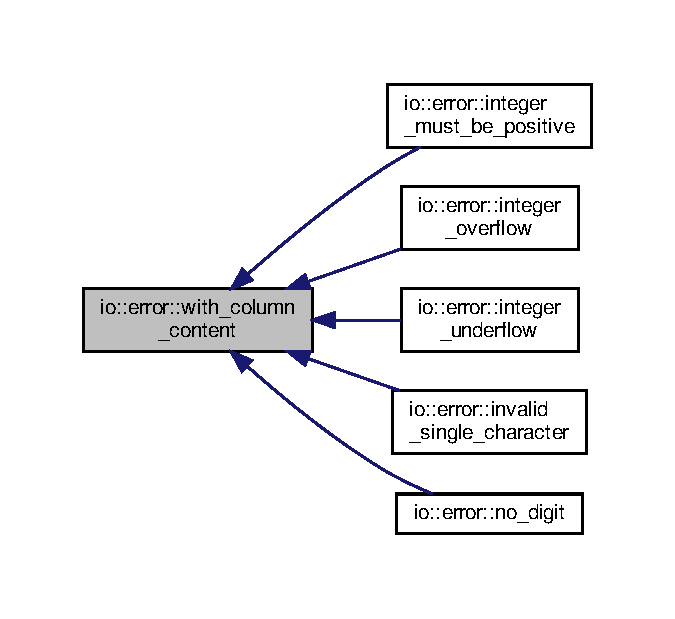
\includegraphics[width=324pt]{structio_1_1error_1_1with__column__content__inherit__graph}
\end{center}
\end{figure}
\subsection*{Public Member Functions}
\begin{DoxyCompactItemize}
\item 
\mbox{\Hypertarget{structio_1_1error_1_1with__column__content_ae7375310dc02425cb3cc4115b3ac8d6a}\label{structio_1_1error_1_1with__column__content_ae7375310dc02425cb3cc4115b3ac8d6a}} 
void {\bfseries set\+\_\+column\+\_\+content} (const char $\ast$column\+\_\+content)
\end{DoxyCompactItemize}
\subsection*{Public Attributes}
\begin{DoxyCompactItemize}
\item 
\mbox{\Hypertarget{structio_1_1error_1_1with__column__content_a8587779769fbfb40155abb362137a523}\label{structio_1_1error_1_1with__column__content_a8587779769fbfb40155abb362137a523}} 
char {\bfseries column\+\_\+content} \mbox{[}max\+\_\+column\+\_\+content\+\_\+length+1\mbox{]}
\end{DoxyCompactItemize}


The documentation for this struct was generated from the following file\+:\begin{DoxyCompactItemize}
\item 
/home/emanuele/catkin\+\_\+ws/src/ros\+\_\+float/include/ros\+\_\+float/csv.\+h\end{DoxyCompactItemize}

\hypertarget{structio_1_1error_1_1with__column__name}{}\section{io\+:\+:error\+:\+:with\+\_\+column\+\_\+name Struct Reference}
\label{structio_1_1error_1_1with__column__name}\index{io\+::error\+::with\+\_\+column\+\_\+name@{io\+::error\+::with\+\_\+column\+\_\+name}}


Inheritance diagram for io\+:\+:error\+:\+:with\+\_\+column\+\_\+name\+:\nopagebreak
\begin{figure}[H]
\begin{center}
\leavevmode
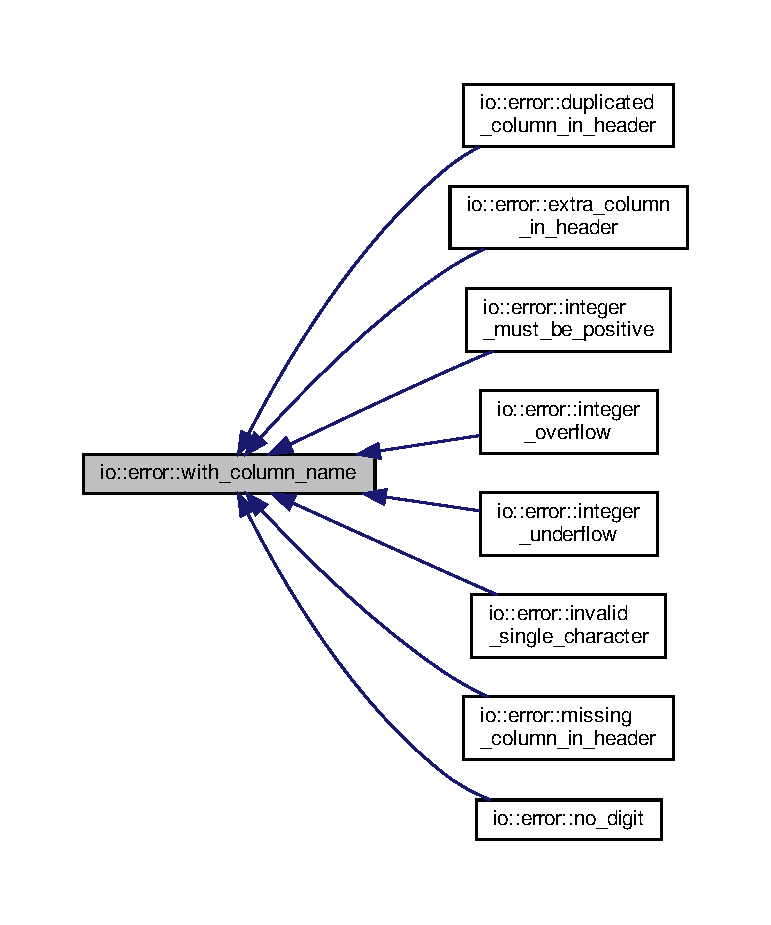
\includegraphics[width=350pt]{structio_1_1error_1_1with__column__name__inherit__graph}
\end{center}
\end{figure}
\subsection*{Public Member Functions}
\begin{DoxyCompactItemize}
\item 
\mbox{\Hypertarget{structio_1_1error_1_1with__column__name_a2a8144d3591a4bb618368ca7261befef}\label{structio_1_1error_1_1with__column__name_a2a8144d3591a4bb618368ca7261befef}} 
void {\bfseries set\+\_\+column\+\_\+name} (const char $\ast$column\+\_\+name)
\end{DoxyCompactItemize}
\subsection*{Public Attributes}
\begin{DoxyCompactItemize}
\item 
\mbox{\Hypertarget{structio_1_1error_1_1with__column__name_af40ba00f1f035d363b099baf1f724323}\label{structio_1_1error_1_1with__column__name_af40ba00f1f035d363b099baf1f724323}} 
char {\bfseries column\+\_\+name} \mbox{[}max\+\_\+column\+\_\+name\+\_\+length+1\mbox{]}
\end{DoxyCompactItemize}


The documentation for this struct was generated from the following file\+:\begin{DoxyCompactItemize}
\item 
/home/emanuele/catkin\+\_\+ws/src/ros\+\_\+float/include/ros\+\_\+float/csv.\+h\end{DoxyCompactItemize}

\hypertarget{structio_1_1error_1_1with__errno}{}\section{io\+:\+:error\+:\+:with\+\_\+errno Struct Reference}
\label{structio_1_1error_1_1with__errno}\index{io\+::error\+::with\+\_\+errno@{io\+::error\+::with\+\_\+errno}}


Inheritance diagram for io\+:\+:error\+:\+:with\+\_\+errno\+:\nopagebreak
\begin{figure}[H]
\begin{center}
\leavevmode
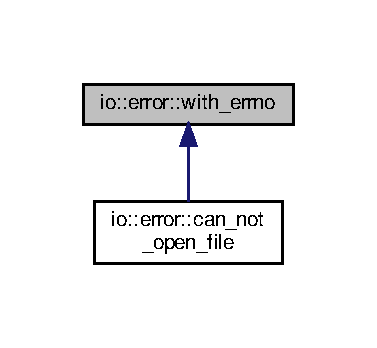
\includegraphics[width=181pt]{structio_1_1error_1_1with__errno__inherit__graph}
\end{center}
\end{figure}
\subsection*{Public Member Functions}
\begin{DoxyCompactItemize}
\item 
\mbox{\Hypertarget{structio_1_1error_1_1with__errno_a572cfa4b4a96792cd1d17dc9ad2eb5a9}\label{structio_1_1error_1_1with__errno_a572cfa4b4a96792cd1d17dc9ad2eb5a9}} 
void {\bfseries set\+\_\+errno} (int errno\+\_\+value)
\end{DoxyCompactItemize}
\subsection*{Public Attributes}
\begin{DoxyCompactItemize}
\item 
\mbox{\Hypertarget{structio_1_1error_1_1with__errno_a99dcacba02cb53351fe64d7e064406be}\label{structio_1_1error_1_1with__errno_a99dcacba02cb53351fe64d7e064406be}} 
int {\bfseries errno\+\_\+value}
\end{DoxyCompactItemize}


The documentation for this struct was generated from the following file\+:\begin{DoxyCompactItemize}
\item 
/home/emanuele/catkin\+\_\+ws/src/ros\+\_\+float/include/ros\+\_\+float/csv.\+h\end{DoxyCompactItemize}

\hypertarget{structio_1_1error_1_1with__file__line}{}\section{io\+:\+:error\+:\+:with\+\_\+file\+\_\+line Struct Reference}
\label{structio_1_1error_1_1with__file__line}\index{io\+::error\+::with\+\_\+file\+\_\+line@{io\+::error\+::with\+\_\+file\+\_\+line}}


Inheritance diagram for io\+:\+:error\+:\+:with\+\_\+file\+\_\+line\+:\nopagebreak
\begin{figure}[H]
\begin{center}
\leavevmode
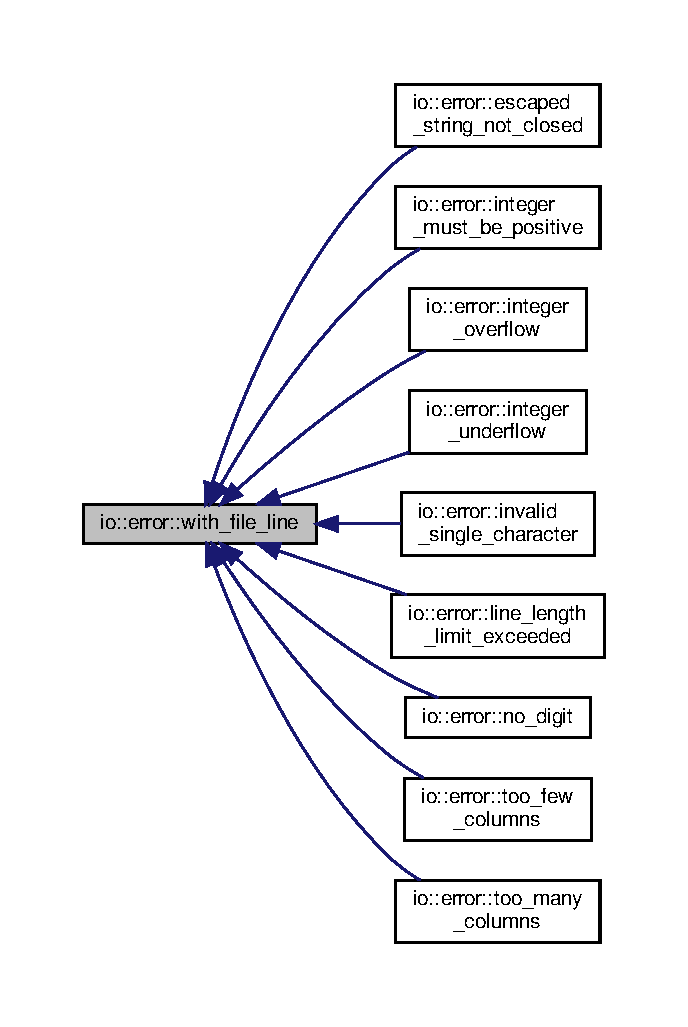
\includegraphics[width=330pt]{structio_1_1error_1_1with__file__line__inherit__graph}
\end{center}
\end{figure}
\subsection*{Public Member Functions}
\begin{DoxyCompactItemize}
\item 
\mbox{\Hypertarget{structio_1_1error_1_1with__file__line_aa92778a81778abc676ec6ee9952bba8c}\label{structio_1_1error_1_1with__file__line_aa92778a81778abc676ec6ee9952bba8c}} 
void {\bfseries set\+\_\+file\+\_\+line} (int file\+\_\+line)
\end{DoxyCompactItemize}
\subsection*{Public Attributes}
\begin{DoxyCompactItemize}
\item 
\mbox{\Hypertarget{structio_1_1error_1_1with__file__line_a391298c37172bcdb83aeb3daf65d5a0e}\label{structio_1_1error_1_1with__file__line_a391298c37172bcdb83aeb3daf65d5a0e}} 
int {\bfseries file\+\_\+line}
\end{DoxyCompactItemize}


The documentation for this struct was generated from the following file\+:\begin{DoxyCompactItemize}
\item 
/home/emanuele/catkin\+\_\+ws/src/ros\+\_\+float/include/ros\+\_\+float/csv.\+h\end{DoxyCompactItemize}

\hypertarget{structio_1_1error_1_1with__file__name}{}\section{io\+:\+:error\+:\+:with\+\_\+file\+\_\+name Struct Reference}
\label{structio_1_1error_1_1with__file__name}\index{io\+::error\+::with\+\_\+file\+\_\+name@{io\+::error\+::with\+\_\+file\+\_\+name}}


Inheritance diagram for io\+:\+:error\+:\+:with\+\_\+file\+\_\+name\+:\nopagebreak
\begin{figure}[H]
\begin{center}
\leavevmode
\includegraphics[height=550pt]{structio_1_1error_1_1with__file__name__inherit__graph}
\end{center}
\end{figure}
\subsection*{Public Member Functions}
\begin{DoxyCompactItemize}
\item 
\mbox{\Hypertarget{structio_1_1error_1_1with__file__name_ae765de62778c989d4658b4efe2995390}\label{structio_1_1error_1_1with__file__name_ae765de62778c989d4658b4efe2995390}} 
void {\bfseries set\+\_\+file\+\_\+name} (const char $\ast$file\+\_\+name)
\end{DoxyCompactItemize}
\subsection*{Public Attributes}
\begin{DoxyCompactItemize}
\item 
\mbox{\Hypertarget{structio_1_1error_1_1with__file__name_ac957d5590a8b95517b74eb5bf373a424}\label{structio_1_1error_1_1with__file__name_ac957d5590a8b95517b74eb5bf373a424}} 
char {\bfseries file\+\_\+name} \mbox{[}max\+\_\+file\+\_\+name\+\_\+length+1\mbox{]}
\end{DoxyCompactItemize}


The documentation for this struct was generated from the following file\+:\begin{DoxyCompactItemize}
\item 
/home/emanuele/catkin\+\_\+ws/src/ros\+\_\+float/include/ros\+\_\+float/csv.\+h\end{DoxyCompactItemize}

%--- End generated contents ---

% Index
\backmatter
\newpage
\phantomsection
\clearemptydoublepage
\addcontentsline{toc}{chapter}{Index}
\printindex

\end{document}
